\documentclass[a4paper]{article}

\def\npart {III}
\def\nterm {Michaelmas}
\def\nyear {2016}
\def\nlecturer {B.\ Allanach}
\def\ncourse {Quantum Field Theory}

\usepackage{myheader}
\usepackage{simplewick}
\usepackage[compat=1.1.0]{tikz-feynman}
\tikzfeynmanset{/tikzfeynman/momentum/arrow shorten = 0.3}
\tikzfeynmanset{/tikzfeynman/warn luatex = false}

\begin{document}
\maketitle
{\small
\setlength{\parindent}{0em}
\setlength{\parskip}{1em}

Quantum Field Theory is the language in which modern particle physics is formulated. It represents the marriage of quantum mechanics with special relativity and provides the mathematical framework in which to describe the interactions of elementary particles.

This first Quantum Field Theory course introduces the basic types of fields which play an important role in high energy physics: scalar, spinor (Dirac), and vector (gauge) fields. The relativistic invariance and symmetry properties of these fields are discussed using Lagrangian language and Noether's theorem.

The quantisation of the basic non-interacting free fields is firstly developed using the Hamiltonian and canonical methods in terms of operators which create and annihilate particles and anti-particles. The associated Fock space of quantum physical states is explained together with ideas about how particles propagate in spacetime and their statistics. How these fields interact with a classical electromagnetic field is described.

Interactions are described using perturbative theory and Feynman diagrams. This is first illustrated for theories with a purely scalar field interaction, and then for a couplings between scalar fields and fermions. Finally Quantum Electrodynamics, the theory of interacting photons, electrons and positrons, is introduced and elementary scattering processes are computed.

\subsubsection*{Pre-requisites}
You will need to be comfortable with the Lagrangian and Hamiltonian formulations of classical mechanics and with special relativity. You will also need to have taken an advanced course on quantum mechanics.
}
\tableofcontents

\setcounter{section}{-1}
\section{Introduction}
%\emph{The greyed out parts are my own attempts to make more sense of the theory from a more mathematical/differential-geometric point of view}

The idea of quantum mechanics is that photons and electrons behave similarly. We can make a photon interfere with itself in double-slit experiments, and similarly an electron can interfere with itself. However, as we know, lights are ripples in an electromagnetic field. So photons should arise from the quantization of the electromagnetic field. If electrons are like photons, should we then have an electron field? The answer is yes!

Quantum field theory is a quantization of a classical field. Recall that in quantum mechanics, we promote degrees of freedom to operators. Basic degrees of freedom of a quantum field theory are operator-valued functions of spacetime. Since there are infinitely many points in spacetime, there is an infinite number of degrees of freedom. This infinity will come back and bite us as we try to develop quantum field theory.

Quantum field theory describes creation and annihilation of particles. The interactions are governed by several basic principles --- locality, symmetry and \emph{renormalization group flow}. What the renormalization group flow describes is the decoupling of low and high energy processes.

\subsubsection*{Why quantum field theory?}
It appears that all particles of the same type are indistinguishable, e.g.\ all electrons are the same. It is difficult to justify why this is the case if each particle is considered individually, but if we view all electrons as excitations of the same field, this is (almost) automatic.

Secondly, if we want to combine special relativity and quantum mechanics, then the number of particles is not conserved. Indeed, consider a particle trapped in a box of size $L$. By the Heisenberg uncertainty principle, we have $\Delta p \gtrsim \hbar/L$. We choose a particle with small rest mass so that $m \ll E$. Then we have
\[
  \Delta E = \Delta p \cdot c \gtrsim \frac{\hbar c}{L}.
\]
When $\Delta E \gtrsim 2 mc^2$, then we can pop a particle-antiparticle pair out of the vacuum. So when $L \lesssim \frac{\hbar}{2mc}$, we can't say for sure that there is only one particle.

We say $\lambda = \hbar/(mc)$ is the ``compton wavelength'' --- the minimum distance at which it makes sense to localize a particle. This is also the scale at which quantum effects kick in.

This argument is somewhat circular, since we just assumed that if we have enough energy, then particle-antiparticle pairs would just pop out of existence. This is in fact something we can prove in quantum field theory.

To reconcile quantum mechanics and special relativity, we can try to write a relativistic version of Schr\"odinger's equation for a single particle, but something goes wrong. Either the energy is unbounded from below, or we end up with some causality violation. This is bad. These are all fixed by quantum field theory by the introduction of particle creation and annihilation.

\subsubsection*{What is quantum field theory good for?}
Quantum field theory is used in (non-relativistic) condensed matter systems. It describes simple phenomena such as phonons, superconductivity, and the fractional quantum hall effect.

Quantum field theory is also used in high energy physics. The standard model of particle physics consists of electromagnetism (quantum electrodynamics), quantum chromodynamics and the weak forces. The standard model is tested to very high precision by experiments, sometimes up to $1$ part in $10^{10}$. So it is good. While there are many attempts to go beyond the standard model, e.g.\ Grand Unified Theories, they are mostly also quantum field theories.

In cosmology, quantum field theory is used to explain the density perturbations. In quantum gravity, string theory is also primarily a quantum field theory in some aspects. It is even used in pure mathematics, with applications in topology and geometry.

\subsubsection*{History of quantum field theory}
In the 1930's, the basics of quantum field theory were laid down by Jordan, Pauli, Heisenberg, Dirac, Weisskopf etc. They encountered all sorts of infinities, which scared them. Back then, these sorts of infinities seemed impossible to work with.

Fortunately, in the 1940's, renormalization and quantum electrodynamics were invented by Tomonaga, Schwinger, Feynman, Dyson, which managed to deal with the infinities. It was a sloppy process, and there was no understanding of why we can subtract infinities and get a sensible finite result. Yet, they managed to make experimental predictions, which were subsequently verified by actual experiments.

In the 1960's, quantum field theory fell out of favour as new particles such as mesons and baryons were discovered. But in the 1970's, it had a golden age when the renormalization group was developed by Kadanoff and Wilson, which was really when the infinities became understood. At the same time, the standard model was invented, and a connection between quantum field theory and geometry was developed.

\subsubsection*{Units and scales}
We are going to do a lot of computations in the course, which are reasonably long. We do not want to have loads of $\hbar$ and $c$'s all over the place when we do the calculations. So we pick convenient units so that they all vanish.

Nature presents us with three fundamental dimensionful constants that are relevant to us:
\begin{enumerate}
  \item The speed of light $c$ with dimensions $LT^{-1}$;
  \item Planck's constant $\hbar$ with dimensions $L^2 MT^{-1}$;
  \item The gravitational constant $G$ with dimensions $L^3 M^{-1} T^{-2}$.
\end{enumerate}
We see that these dimensions are independent. So we define units such that $c = \hbar = 1$. So we can express everything in terms of a mass, or an energy, as we now have $E = m$. For example, instead of $\lambda = \hbar/(mc)$, we just write $\lambda = m^{-1}$. We will work with electron volts $eV$. To convert back to the conventional SI units, we must insert the relevant powers of $c$ and $\hbar$. For example, for a mass of $m_e = \SI{e6}\electronvolt$, we have $\lambda_e = \SI{2e-12}{\meter}$.

After getting rid of all factors of $\hbar$ and $c$, if a quantity $X$ has a mass dimension $d$, we write $[X] = d$. For example, we have $[G] = - 2$, since we have
\[
  G = \frac{\hbar c}{M_p^2} = \frac{1}{M_p^2},
\]
where $M_p \sim \SI{e19}{\giga\electronvolt}$ is the \emph{Planck scale}.

\section{Classical field theory}
Before we get into quantum nonsense, we will first start by understanding classical fields.

\subsection{Classical fields}
\begin{defi}[Field]\index{field}
  A \emph{field} $\phi$ is a physical quantity defined at every point of spacetime $(\mathbf{x}, t)$. We write the value of the field at $(\mathbf{x}, t)$ as $\phi(\mathbf{x}, t)$.
\end{defi}
The ``physical quantities'' can be real or complex scalars, but later we will see that we might have to consider even more complicated stuff.

In classical point mechanics, we have a finite number of generalized coordinates $q_a(t)$. In field theory, we are interested in the dynamics of $\phi_a(\mathbf{x}, t)$, where $a$ and $\mathbf{x}$ are \emph{both} labels. Here the $a$ labels the different fields we can have, and $(\mathbf{x}, t)$ labels a spacetime coordinate. Note that here position has been relegated from a dynamical variable (i.e.\ one of the $q_a$) to a mere label.

\begin{eg}
  The \term{electric field} $E_i(\mathbf{x}, t)$ and \term{magnetic field} $B_i(\mathbf{x}, t)$, for $i = 1, 2, 3$, are examples of fields. These six fields can in fact be derived from 4 fields $A_\mu(\mathbf{x}, t)$, for $\mu = 0, 1, 2, 3$, where
  \[
    E_i = \frac{\partial A_i}{\partial t} - \frac{\partial A_0}{\partial x_i},\quad B_i = \frac{1}{2} \varepsilon_{ijk}\frac{\partial A_k}{\partial x^j}.
  \]
  Often, we write
  \[
    A^\mu = (\phi, \mathbf{A}).
  \]
\end{eg}

Just like in classical dynamics, we would specify the dynamics of a field through a \emph{Lagrangian}. For particles, the Lagrangian specifies a number at each time $t$. Since a field is a quantity at each point in space, we now have Lagrangian \emph{densities}, which gives a number at each point in spacetime $(t, \mathbf{x})$.

\begin{defi}[Lagrangian density]\index{Lagrangian density}
  Given a field $\phi (\mathbf{x}, t)$, a \emph{Lagrangian density} is a function $\mathcal{L}(\phi, \partial_\mu \phi)$ of $\phi$ and its derivative.
\end{defi}

Note that the Lagrangian density treats space and time symmetrically. However, if we already have a favorite time axis, we can look at the ``total'' Lagrangian at each time, and obtain what is known as the \emph{Lagrangian}.

\begin{defi}[Lagrangian]\index{Lagrangian}
  Given a Lagrangian density, the \emph{Lagrangian} is defined by
  \[
    L = \int \d^3 \mathbf{x}\; \mathcal{L}(\phi, \partial_\mu \phi).
  \]
\end{defi}
For most of the course, we will only care about the Lagrangian density, and call it the Lagrangian.

\begin{defi}[Action]\index{action}
  Given a Lagrangian and a time interval $[t_1, t_2]$, the \emph{action} is defined by
  \[
    S = \int_{t_1}^{t_2} \;\d t\; L(t) = \int \d^4 x\; \mathcal{L}.
  \]
\end{defi}
In general, we would want the units to satisfy $[S] = 0$. Since we have $[\d^4 x] = -4$, we must have $[\mathcal{L}] = 4$.

The equations of motion are, as usual, given by the principle of least action.
\begin{defi}[Principle of least action]\index{principle of least action}
  The equation of motion of a Lagrangian system is given by the \emph{principle of least action} --- we vary the field slightly, keeping values at the boundary fixed, and require the first-order change $\delta S = 0$.
\end{defi}

For a small perturbation $\phi_a \mapsto \phi_a + \delta \phi_a$, we can compute
\begin{align*}
  \delta S &= \int \d^4 x\left(\frac{\partial \mathcal{L}}{\partial \phi_a} \delta \phi_a + \frac{\partial \mathcal{L}}{\partial (\partial_\mu \phi_a)} \delta(\partial_\mu\phi_a)\right)\\
  &= \int \d^4 x \left\{\left(\frac{\partial \mathcal{L}}{\partial \phi_a} - \partial_\mu\left(\frac{\partial \mathcal{L}}{\partial (\partial_\mu\phi_a)}\right)\right) \delta \phi_a + \partial_\mu \left(\frac{\partial \mathcal{L}}{\partial (\partial_\mu\phi_a)} \delta\phi_a\right)\right\}.
\end{align*}
We see that the last term vanishes for any term that decays at spatial infinity, and obeys $\delta \phi_a(\mathbf{x}, t_1) = \delta\phi_a(\mathbf{x}, t_2) = 0$.

Requiring $\delta S = 0$ means that we need
\begin{prop}[Euler-Lagrange equations]
  The equations of motion for a field are given by the \term{Euler-Lagrange equations}:
  \[
    \partial_\mu\left(\frac{\partial \mathcal{L}}{\partial (\partial_\mu \phi_a)}\right) - \frac{\partial \mathcal{L}}{\partial \phi_a} = 0.
  \]
\end{prop}

We can begin by considering the simplest field one can imagine of --- the Klein--Gordon field. We will later see that this is a ``free field'', and ``particles'' don't interact with each other.

\begin{eg}
  The \term{Klein--Gordon equation} for a real scalar field $\phi(\mathbf{x}, t)$ is given by the Lagrangian
  \[
    \mathcal{L} = \frac{1}{2} \partial_\mu \phi \partial^\mu \phi - \frac{1}{2}m^2 \phi^2 = \frac{1}{2} \dot{\phi}^2 - \frac{1}{2} (\nabla \phi)^2 - \frac{1}{2} m^2 \phi^2.
  \]
  We can view this Lagrangian as saying $\mathcal{L} = T - V$, where
  \[
    T = \frac{1}{2} \dot{\phi}^2
  \]
  is the kinetic energy, and
  \[
    V = \frac{1}{2} (\nabla \phi)^2 + \frac{1}{2}m^2 \phi^2
  \]
  is the potential energy.

  To find the Euler-Lagrange equation, we can compute
  \[
    \frac{\partial \mathcal{L}}{\partial(\partial_\mu \phi)} = \partial^\mu \phi = (\dot{\phi}, -\nabla \phi)
  \]
  and
  \[
    \frac{\partial \mathcal{L}}{\partial \phi} = -m^2 \phi.
  \]
  So the Euler-Lagrange equation says
  \[
    \partial_\mu \partial^\mu \phi + m^2 \phi = 0.
  \]
  More explicitly, this says
  \[
    \ddot{\phi} - \nabla^2 \phi + m^2 \phi = 0.
  \]
\end{eg}
We could generalize this and add more terms to the Lagrangian. An obvious generalization would be
\[
  \mathcal{L} = \frac{1}{2} \partial_\mu \phi \partial^\mu \phi - V(\phi),
\]
where $V(\phi)$ is an arbitrary potential function. Then we similarly obtain the equation
\[
  \partial_\mu \partial^\mu \phi + \frac{\partial V}{\partial \phi} = 0.
\]

\begin{eg}
  \term{Maxwell's equations} in vacuum are given by the Lagrangian
  \[
    \mathcal{L} = -\frac{1}{2} (\partial_\mu A_\nu)(\partial^\mu A^\nu) + \frac{1}{2}(\partial_\mu A^\mu)^2.
  \]
  To find out the Euler-Lagrange equations, we need to figure out the derivatives with respect to each component of the $A$ field. We obtain
  \[
    \frac{\partial \mathcal{L}}{\partial(\partial_\mu A_\nu)} = -\partial^\mu A^\nu + (\partial_\rho A^\rho) \eta^{\mu\nu}.
  \]
  So we obtain
  \[
    \partial_\mu \left(\frac{\partial \mathcal{L}}{\partial(\partial_\mu A_\nu)}\right) = - \partial_\mu\partial^\mu A^\nu + \partial^\nu (\partial_\rho A^\rho) = - \partial_\mu (\partial^\mu A^\nu - \partial^\nu A^\mu).
  \]
  We write
  \[
    F^{\mu\nu} = \partial^\mu A^\nu - \partial^\nu A^\mu.
  \]
  So we are left with
  \[
    \partial_\mu \left(\frac{\partial \mathcal{L}}{\partial(\partial_\mu A_\nu)}\right) = -\partial_\mu F^{\mu\nu}.
  \]
  It is an exercise to check that these Euler-Lagrange equations reproduce
  \[
    \partial_i E_i = 0,\quad \dot{E}_i = \varepsilon_{ijk} \partial_j B_k.
  \]
  Using our $F^{\mu\nu}$, we can rewrite the Lagrangian as
  \[
    \mathcal{L} = -\frac{1}{4} F_{\mu\nu}F^{\mu\nu}.
  \]
\end{eg}
How did we come up with these Lagrangians? In general, it is guided by two principles --- one is symmetry, and the other is renormalizability. We will discuss symmetries shortly, and renormalizaility would be done in the III Advanced Quantum Field Theory course.

In all of these examples, the Lagrangian is local. In other words, the terms don't couple $\phi(\mathbf{x}, t)$ to $\phi(\mathbf{y}, t)$ if $\mathbf{x} \not= \mathbf{y}$.
\begin{eg}
  An example of a non-local Lagrangian would be
  \[
    \int \d^3 \mathbf{x} \int \d^3 \mathbf{y} \; \phi(\mathbf{x}) \phi(\mathbf{x} - \mathbf{y})
  \]
\end{eg}
A priori, there is no reason for this, but it happens that nature seems to be local. So we shall only consider local Lagrangians.

Note that locality does \emph{not} mean that the Lagrangian at a point only depends on the value at the point. Indeed, it also depends on the derivatives at $\mathbf{x}$. So we can view this as saying the value of $\mathcal{L}$ at $\mathbf{x}$ only depends on the value of $\phi$ at an infinitesimal neighbourhood of $\mathbf{x}$ (formally, the jet at $\mathbf{x}$).

\subsection{Lorentz invariance}
If we wish to construct relativistic field theories such that $\mathbf{x}$ and $t$ are on an equal footing, the Lagrangian should be invariant under \term{Lorentz transformations} $x^\mu \mapsto x'^\mu = \Lambda^\mu\!_\nu x^\nu$, where
\[
  \Lambda^\mu\!_\sigma \eta^{\sigma\tau} \Lambda^\nu\!_\tau = \eta^{\mu\nu}.
\]
and $\eta^{\mu\nu}$ is the \term{Minkowski metric} given by
\[
  \eta^{\mu\nu} =
  \begin{pmatrix}
    1 & 0 & 0 & 0\\
    0 & -1 & 0 & 0\\
    0 & 0 & -1 & 0\\
    0 & 0 & 0 & -1
  \end{pmatrix}.
\]

\begin{eg}
  The transformation
  \[
    \Lambda^\mu\!_\sigma =
    \begin{pmatrix}
      1 & 0 & 0 & 0\\
      0 & 1 & 0 & 0\\
      0 & 0 & \cos \theta & -\sin \theta\\
      0 & 0 & \sin \theta & \cos \theta
    \end{pmatrix}
  \]
  describes a rotation by an angle around the $x$-axis.
\end{eg}

\begin{eg}
  The transformation
  \[
    \Lambda^\mu\!_\sigma =
    \begin{pmatrix}
      \gamma & -\gamma v & 0 & 0\\
      -\gamma v & \gamma & 0 & 0\\
      0 & 0 & 1 & 0\\
      0 & 0 & 0 & 1
    \end{pmatrix}
  \]
  describes a \term{boost} by $v$ along the $x$-axis.
\end{eg}
The Lorentz transformations form a Lie group under matrix multiplication --- see III Symmetries, Field and Particles.

The Lorentz transformations have a representation on the fields. For a scalar field, this is given by
\[
  \phi(x) \mapsto \phi'(x) = \phi(\Lambda^{-1}x),
\]
where the indices are suppressed. This is an active transformation --- say $x_0$ is the point at which, say, the field is a maximum. Then after applying the Lorentz transformation, the position of the new maximum is $\Lambda x_0$. The field itself actually moved.

Alternatively, we can use passive transformations, where we just relabel the points. In this case, we have
\[
  \phi(x) \mapsto \phi(\Lambda (x)).
\]
However, this doesn't really matter, since if $\Lambda$ is a Lorentz transformation, then so is $\Lambda^{-1}$. So being invariant under active transformations is the same as being invariant under passive transformations.

A Lorentz invariant theory should have equations of motion such that if $\phi(x)$ is a solution, then so is $\phi(\Lambda^{-1} x)$. This can be achieved by requiring that the action $S$ is invariant under Lorentz transformations.

\begin{eg}
  In the Klein--Gordon field, we have
  \[
    \mathcal{L} = \frac{1}{2} \partial_\mu \phi \partial^\mu \phi - \frac{1}{2}m^2 \phi^2.
  \]
  The Lorentz transformation is given by
  \[
    \phi(x) \mapsto \phi'(x) = \phi(\Lambda^{-1}x) = \phi(y),
  \]
  where
  \[
    y^\mu = (\Lambda^{-1})^\mu\!_\nu x^\nu.
  \]
  We then check that
  \begin{align*}
    \partial_\mu \phi(x) &\mapsto \frac{\partial}{\partial x^\mu}(\phi(\Lambda^{-1}x)) \\
    &= \frac{\partial}{\partial x^\mu} (\phi(y))\\
    &= \frac{\partial y^\nu}{\partial x^\mu} \frac{\partial}{\partial y^\nu} (\phi(y))\\
    &= (\Lambda^{-1})^\nu\!_\mu(\partial_\nu \phi)(y).
  \end{align*}
  Since $\Lambda^{-1}$ is a Lorentz transformation, we have
  \[
    \partial_\mu \phi \partial^\mu \phi = \partial_\mu \phi' \partial^\mu \phi'.
  \]
\end{eg}
In general, as long as we write everything in terms of tensors, we get Lorentz invariant theories.

Symmetries play an important role in QFT. Different kinds of symmetries include Lorentz symmetries, gauge symmetries, global symmetries and supersymmetries (SUSY).

\begin{eg}
  Protons and neutrons are made up of quarks. Each type of quark comes in three flavors, which are called red, blue and green (these are arbitrary names). If we swap around red and blue everywhere in the universe, then the laws don't change. This is known as a global symmetry.

  However, in light of relativity, swapping around red and blue \emph{everywhere} in the universe might be a bit absurd, since the universe is so big. What if we only do it locally? If we make the change differently at different points, the equations don't \emph{a priori} remain invariant, unless we introduce a \emph{gauge boson}. More of this will be explored in the AQFT course.
\end{eg}

\subsection{Symmetries and Noether's theorem for field theories}
As in the case of classical dynamics, we get a Noether's theorem that tells us symmetries of the Lagrangian give us conserved quantities. However, we have to be careful here. If we want to treat space and time equally, saying that a quantity ``does not change in time'' is bad. Instead, what we have is a \emph{conserved current}, which is a $4$-vector. Then given any choice of spacetime frame, we can integrate this conserved current over all space at each time (with respect to the frame), and this quantity will be time-invariant.

\begin{thm}[Noether's theorem]\index{Noether's theorem}
  Every continuous symmetry of $\mathcal{L}$ gives rise to a \term{conserved current} $j^\mu(x)$ such that the equation of motion implies that
  \[
    \partial_\mu j^\mu = 0.
  \]
  More explicitly, this gives
  \[
    \partial_0 j^0 + \nabla \cdot \mathbf{j} = 0.
  \]
  A conserved current gives rise to a \emph{conserved charge}
  \[
    Q = \int_{\R^3} j^0 \d^3 \mathbf{x},
  \]
  since
  \begin{align*}
    \frac{\d Q}{\d t} &= \int_{\R^3} \frac{\d j^0}{\d t} \;\d^3 \mathbf{x}\\
    &= -\int_{\R^3} \nabla \cdot \mathbf{j} \;\d ^3 \mathbf{x}\\
    &= 0,
  \end{align*}
  assuming that $j^i \to 0$ as $|\mathbf{x}| \to \infty$.
\end{thm}

\begin{proof}
  Consider making an arbitrary transformation of the field $\phi_a \mapsto \phi_a + \delta \phi_a$. We then have
  \begin{align*}
    \delta \mathcal{L} &= \frac{\partial \mathcal{L}}{\partial \phi_a} \delta \phi_a + \frac{\partial \mathcal{L}}{\partial(\partial_\mu \phi_a)} \delta(\partial_\mu \phi_a)\\
    &= \left[\frac{\partial \mathcal{L}}{\partial \phi_a} - \partial_\mu \frac{\partial \mathcal{L}}{\partial(\partial_\mu \phi_a)}\right] \delta \phi_a + \partial_\mu \left(\frac{\partial \mathcal{L}}{\partial(\partial_\mu \phi_a)} \delta \phi_a\right).
  \end{align*}
  When the equations of motion are satisfied, we know the first term always vanishes. So we are left with
  \[
    \delta \mathcal{L} = \partial_\mu \left(\frac{\partial \mathcal{L}}{\partial(\partial_\mu \phi_a)} \delta \phi_a\right).
  \]
  If the specific transformation $\delta \phi_a = X_a$ we are considering is a \term{symmetry}, then $\delta\mathcal{L} = 0$ (this is the definition of a symmetry). In this case, we can define a conserved current by
  \[
    j^\mu = \frac{\partial \mathcal{L}}{\partial (\partial_\mu \phi_a)}X_a,
  \]
  and by the equations above, this is actually conserved.
\end{proof}
We can have a slight generalization where we relax the condition for a symmetry and still get a conserved current. We say that $X_a$ is a symmetry if $\delta \mathcal{L} = \partial_\mu F^\mu(\phi)$ for some $F^\mu(\phi)$, i.e.\ a total derivative. Replaying the calculations, we get
\[
  j^\mu = \frac{\partial \mathcal{L}}{\partial (\partial_\mu \phi_a)} X_a - F^\mu.
\]
\begin{eg}[Space-time invariance]
  Recall that in classical dynamics, spatial invariance implies the conservation of momentum, and invariance wrt to time translation implies the conservation of energy. We'll see something similar in field theory. Consider $x^\mu \mapsto x^\mu - \varepsilon^\mu$. Then we obtain
  \[
    \phi_a(x) \mapsto \phi_a(x) + \varepsilon^\nu \partial_\nu \phi_a(x).
  \]
  A Lagrangian that has no explicit $x^\mu$ dependence transforms as
  \[
    \mathcal{L}(x) \mapsto \mathcal{L}(x) + \varepsilon^\nu \partial_\nu \mathcal{L}(x),
  \]
  giving rise to 4 currents --- one for each $\nu = 0, 1, 2, 3$. We have
  \[
    (j^\mu)_\nu = \frac{\partial \mathcal{L}}{\partial (\partial_\mu \phi_a)} \partial_\nu \phi_a - \delta^\mu\!_\nu \mathcal{L},
  \]
  This particular current is called $T^\mu\!_\nu$, the \term{energy-momentum tensor}\index{$T^\mu_\nu$}. This satisfies
  \[
    \partial_\mu T^\mu\!_\nu = 0,
  \]
  We obtain conserved quantities, namely the \term{energy}
  \[
    E = \int \d^3 \mathbf{x}\;T^{00},
  \]
  and the total \term{momentum}
  \[
    \mathbf{P}^i = \int \d^3 \mathbf{x}\; T^{0i}.
  \]
\end{eg}

\begin{eg}
  Consider the Klein--Gordon field, with
  \[
    \mathcal{L} = \frac{1}{2} \partial_\mu \phi \partial^\mu \phi - \frac{1}{2}m^2 \phi^2.
  \]
  We then obtain
  \[
    T^{\mu\nu} = \partial^\mu \phi \partial^\nu \phi - \eta^{\mu\nu} \mathcal{L}.
  \]
  So we have
  \[
    E = \int \d^3 \mathbf{x} \left(\frac{1}{2}\dot{\phi}^2 + \frac{1}{2}(\nabla \phi)^2 + \frac{1}{2}m^2 \phi^2\right).
  \]
  The momentum is given by
  \[
    \mathbf{P}^i = \int\d^3 \mathbf{x}\; \dot{\phi} \partial^i \phi.
  \]
\end{eg}
In this example, $T^{\mu\nu}$ comes out symmetric in $\mu$ and $\nu$. In general, it would not be, but we can always massage it into a symmetric form by adding
\[
  \sigma^{\mu\nu} = T^{\mu\nu} + \partial_\rho \Gamma^{\rho\mu\nu}
\]
with $\Gamma^{\rho\mu\nu}$ a tensor antisymmetric in $\rho$ and $\mu$. Then we have
\[
  \partial_\mu \partial_\rho \Gamma^{\rho\mu\nu} = 0.
\]
So this $\sigma^{\mu\nu}$ is also invariant.

A symmetric energy-momentum tensor of this form is actually useful, and is found on the RHS of Einstein's field equation.

\begin{eg}[Internal symmetries]
  Consider a complex scalar field
  \[
    \psi(x) = \frac{1}{\sqrt{2}} (\phi_1(x) + i \phi_2(x)),
  \]
  where $\phi_1$ and $\phi_2$ are real scalar fields. We put
  \[
    \mathcal{L} = \partial_\mu \psi^* \partial^\mu \psi - V(\psi^*\psi),
  \]
  where
  \[
    V (\psi^*\psi) = m^2 \psi^* \psi + \frac{\lambda}{2}(\psi^*\psi)^2 + \cdots
  \]
  is some potential term.

  To find the equations of motion, if we do all the complex analysis required, we will figure that we will obtain the same equations as the real case if we treat $\psi$ and $\psi^*$ as independent variables. In this case, we obtain
  \[
    \partial_\mu \partial^\mu \psi + m^2 \psi + \lambda (\psi^*\psi) \psi + \cdots = 0
  \]
  and its complex conjugate.
  The $\mathcal{L}$ has a symmetry given by $\psi \mapsto e^{i\alpha} \psi$. Infinitesimally, we have $\delta \psi = i\alpha \psi$, and $\delta \psi^* = -i\alpha \psi^*$.

  This gives a current
  \[
    j^\mu = i(\partial^\mu \psi^*) \psi - i (\partial^\mu \psi)\psi^*.
  \]
  We will later see that associated charges of this type have an interpretation of electric charge (or particle number, e.g.\ baryon number or lepton number).
\end{eg}

Note that this symmetry is an abelian symmetry, since it is a symmetry under the action of the abelian group $\U(1)$. There is a generalization to a non-abelian case.

\begin{eg}[Non-abelian internal symmetries]
  Suppose we have a theory with many fields, with the Lagrangian given by
  \[
    \mathcal{L} = \frac{1}{2} \sum_{a = 1}^N \partial_\mu \phi_a \partial^\mu \phi_a - \frac{1}{2} \sum_{a = 1}^N m^2 \phi_a^2 - g \left(\sum_{a = 1}^N \phi_a^2\right)^2.
  \]
  This theory is invariant under the bigger symmetry group $G = \SO(N)$. If we view the fields as components of complex fields, then we have a symmetry under $\U(N/2)$ or even $\SU(N/2)$. For example, the symmetry group $\SU(3)$ gives the \term{8-fold way}.
\end{eg}

\begin{eg}
  There is a nice trick to determine the conserved current when our infinitesimal transformation is given by $\delta \phi = \alpha \phi$ for some real constant $\alpha$. Consider the case where we have an \emph{arbitrary} perturbation $\alpha = \alpha(x)$. In this case, $\delta\mathcal{L}$ is no longer invariant, but we know that whatever formula we manage to come up with, it has to vanish when $\alpha$ is constant. Assuming that we only have first-order derivatives, the change in Lagrangian must be of the form
  \[
    \delta \mathcal{L} = (\partial_\mu \alpha(x)) h^\mu(\phi).
  \]
  for some $h^\mu$. We claim that $h^\mu$ is the conserved current. Indeed, we have
  \[
    \delta S = \int \d^4 x\; \delta \mathcal{L} = - \int \d^4 x\; \alpha(x) \partial_\mu h^\mu,
  \]
  using integration by parts. We know that if the equations of motion are satisfied, then this vanishes for any $\alpha(x)$ as long as it vanishes at infinity (or the boundary). So we must have
  \[
    \partial_\mu h^\mu = 0.
  \]
\end{eg}

\subsection{Hamiltonian mechanics}
We can now talk about the Hamiltonian formulation. This can be done for field theories as well. We define
\begin{defi}[Conjugate momentum]\index{conjugate momentum}
  Given a Lagrangian system for a field $\phi$, we define the \emph{conjugate momentum} by
  \[
    \pi(x) = \frac{\partial \mathcal{L}}{\partial \dot{\phi}}.
  \]
\end{defi}
This is not to be confused with the total momentum $\mathbf{P}^i$.

\begin{defi}[Hamiltonian density]\index{Hamiltonian density}
  The \emph{Hamiltonian density} is given by
  \[
    \mathcal{H} = \pi(x) \dot{\phi}(x) - \mathcal{L}(x),
  \]
  where we replace all occurrences of $\dot{\phi}(x)$ by expressing it in terms of $\pi(x)$.
\end{defi}

\begin{eg}
  Suppose we have a field Lagrangian of the form
  \[
    \mathcal{L} = \frac{1}{2} \dot{\phi}^2 - \frac{1}{2} (\nabla \phi)^2 - V(\phi).
  \]
  Then we can compute that
  \[
    \pi = \dot\phi.
  \]
  So we can easily find
  \[
    \mathcal{H} = \frac{1}{2}\pi^2 + \frac{1}{2}(\nabla \phi)^2 + V(\phi).
  \]
\end{eg}

\begin{defi}[Hamiltonian]\index{Hamiltonian}
  The \emph{Hamiltonian} of a Hamiltonian system is
  \[
    H = \int\;\d^3 \mathbf{x}\; \mathcal{H}.
  \]
\end{defi}
This agrees with the field energy we computed using Noether's theorem.

\begin{defi}[Hamilton's equations]\index{Hamilton's equations}
  Hamilton's equations are
  \[
    \dot{\phi} = \frac{\partial \mathcal{H}}{\partial \pi},\quad \dot{\pi} = -\frac{\partial \mathcal{H}}{\partial \phi}.
  \]
  These give us the equations of motion of $\phi$.
\end{defi}
There is an obvious problem with this, that the Hamiltonian formulation is not manifestly Lorentz invariant. However, we know it actually is because we derived it as an equivalent formulation of a Lorentz invariant theory. So we are safe, so far. We will later have to be more careful if we want to quantize the theories from the Hamiltonian formalism.


%\subsection{Formal point of view*}
%\begin{own}
% Formally, we suppose the universe is given by a spacetime manifold $\mathcal{M}$ with a pseudo-Riemannian metric of signature $(+1, -1, -1 ,-1)$. All maps are assumed to be smooth.
%
% A field can then be defined as a function $\mathcal{M} \to V$, where $V$ is some vector space. This is, of course, equivalent to a section of the trivial bundle $V \times \mathcal{M} \to \mathcal{M}$. A natural generalization would be to define a field as a section of some bundle, and we will consider more general bundles later when we do gauge theory.
%
% Given a vector space $V$, we can define a corresponding (local) Lagrangian density by a function from the $n$th jet bundle $\mathcal{L}: j^n(\mathcal{M}, V) \to \R$ ($n$ can be taken to be infinite if one is not taunted by the horrors of infinite-dimensional spaces). Given a field $\phi: \mathcal{M} \to V$, we write $\mathcal{L}(\phi)$ for the composition $\mathcal{L} \circ j^n \phi$, where $j^n$ is the $n$th jet prolongation of $\phi$. It happens that nature seems to prefer Lagrangians with $n = 1$, and this is the only case we will consider.
%
% If we have found ourselves a preferred time axis $T$, then we can project each spacetime coordinate to the time axis via $\pi: \mathcal{M} \to T$. Given a field $\phi: \mathcal{M} \to V$, we can integrating $\mathcal{L}(\phi)$ along fibers to get the ``total'' Lagrangian at each point in time, and this gives a function $L: T \to V$. This is called the \emph{Lagrangian}.
%
% If we have a $V$ and a Lagrangian density $\mathcal{L}$, the principle of least action the ``allowed'' fields (i.e.\ the fields that will physically exist) are those $\phi:\mathcal{M} \to V$ satisfying the following property:
%
% For any compact region $C \subseteq \mathcal{M}$ and any $F: C \times (-\varepsilon, \varepsilon) \to V$ such that $F(\mathbf{x}, 0) = \phi(\mathbf{x})$ for all $\mathbf{x} \in C$, and $F(\mathbf{x}, s) = \phi(\mathbf{x})$ for all $\mathbf{x} \in \partial C$, we have
% \[
% 0 = \left.\frac{\d}{\d s}\right|_{s = 0} \int_C \d^4 x\; \mathcal{L}(F(\mathbf{x}, s)).
% \]
% We can now define symmetries of the Lagrangian as follows:
% \begin{defi}[Continuous symmetry]\index{continuous symmetry}
% A \emph{continuous symmetry} of the Lagrangian is an action of a Lie group $G$ on $j^n(\mathcal{M}, V)$ such that for every $g \in G$ and every compact set $C \subseteq \mathcal{M}$, we have
% \[
% \int_C \mathcal{L}(j^1\phi(\mathbf{x})) \;\d g = \int_C \mathcal{L}(g \cdot (j^1\phi(\mathbf{x})))\;\d g.
% \]
% In particular, if $L(g \cdot a) = L(a)$ for all $a \in j^n(\mathcal{M}, V)$, then this is a symmetry.
%
% A \emph{one-parameter symmetry} is one where the Lie algebra of $G$ is $\R$.
% \end{defi}
%\end{own}
%
\section{Free field theory}
So far, we've just been talking about classical field theory. We now want to quantize this, and actually do \emph{quantum} field theory.
\subsection{Review of simple harmonic oscillator}
Michael Peskin once famously said ``Physics is the subset of human experience that can be reduced to coupled harmonic oscillators''. Thus, to understand quantum mechanics, it is important to understand how the quantum harmonic oscillator works.

Classically, the simple harmonic oscillator is given by the Hamiltonian
\[
  H = \frac{1}{2}p^2 + \frac{1}{2} \omega^2 q^2,
\]
where $p$ is the momentum and $q$ is the position. To obtain the corresponding quantum system, \term{canonical quantization} tells us that we should promote the $p$ and $q$ into complex ``operators'' $\hat{p}, \hat{q}$, and use the same formula for the Hamiltonian, namely we now have
\[
  \hat{H} = \frac{1}{2}\hat{p}^2 + \frac{1}{2} \omega^2 \hat{q}^2.
\]
In the classical system, the quantities $p$ and $q$ used to satisfy the Poisson brackets
\[
  \{q, p\} = 1.
\]
After promoting to operators, they satisfy the commutation relation
\[
  [\hat{q}, \hat{p}] = i.
\]
We will soon stop writing the hats because we are lazy.

There are a few things to take note of.
\begin{enumerate}
  \item We said $p$ and $q$ are ``operators'', but did not say what they actually operate on! Instead, what we are going to do is to analyze these operators formally, and after some careful analysis, we show that there is a space the operators naturally act on, and then take that as our state space. This is, in general, how we are going to do quantum field theory (except we tend to replace the word ``careful'' with ``sloppy'').

    During the analysis, we will suppose there are indeed some states our operators act on, and then try to figure out what properties the states must have.

  \item The process of canonical quantization depends not only on the classical system itself, but how we decide the present our system. There is no immediate reason why if we pick different coordinates for our classical system, the resulting quantum system would be equivalent. In particular, before quantization, all the terms commute, but after quantization that is no longer true. So how we decide to order the terms in the Hamiltonian matters.

    Later, we will come up with the notion of \emph{normal ordering}. From then onwards, we can have a (slightly) more consistent way of quantizing operators.
\end{enumerate}

After we've done this, the time evolution of states is governed by the Schr\"odinger equation:
\[
  i\frac{\d}{\d t}\bket{\psi} = H\bket{\psi}.
\]
In practice, instead of trying to solve this thing, we want to find eigenstates $\bket{E}$ such that
\[
  H \bket{E} = E\bket{E}.
\]
If such states are found, then defining
\[
  \bket{\psi} = e^{-iEt}\bket{E}
\]
would give a nice, stable solution to the Schr\"odinger equation.

The trick is to notice that in the classical case, we can factorize the Hamiltonian as
\[
  H = \omega \left(\sqrt{\frac{\omega}{2}}q + \frac{i}{\sqrt{2\omega}}p\right)\left(\sqrt{\frac{\omega}{2}}q + \frac{-i}{\sqrt{2\omega}}p\right).
\]
Now $H$ is a product of two terms that are complex conjugates to each other, which, in operator terms, means they are adjoints. So we have the benefit that we only have to deal with a single complex object $\sqrt{\frac{\omega}{2}}q + \frac{i}{\sqrt{2\omega}}p$ (and its conjugate), rather than two unrelated real objects. Also, products are nicer than sums. (if this justification for why this is a good idea doesn't sound convincing, just suppose that we had the idea of doing this via divine inspiration, and it turns out to work well)

We now do the same factorization in the quantum case. We would not expect the result to be \emph{exactly} the above, since that working relies on $p$ and $q$ commuting. However, we can still try and define the operators
\[
  a = \frac{i}{\sqrt{2 \omega}}p + \sqrt{\frac{\omega}{2}}q,\quad a^\dagger = \frac{-i}{\sqrt{2\omega}}p + \sqrt{\frac{\omega}{2}}q.
\]
These are known as \term{creation} and \term{annihilation} operators for reasons that will become clear soon.

We can invert these to find
\[
  q = \frac{1}{\sqrt{2\omega}}(a + a^\dagger),\quad p = -i\sqrt{\frac{\omega}{2}} (a - a^\dagger).
\]
We can substitute these equations into the commutator relation to obtain
\[
  [a, a^\dagger] = 1.
\]
Putting them into the Hamiltonian, we obtain
\[
  H = \frac{1}{2}\omega(a a^\dagger + a^\dagger a) = \omega\left(a^\dagger a + \frac{1}{2}[a, a^\dagger]\right) = \omega \left(a^\dagger a + \frac{1}{2}\right).
\]
We can now compute
\[
  [H, a^\dagger] = \omega a^\dagger,\quad [H, a] = -\omega a.
\]
These ensure that $a, a^\dagger$ take us between energy eigenstates --- if
\[
  H\bket{E} = E \bket{E},
\]
then
\[
  Ha^\dagger\bket{E} = (a^\dagger H + [H, a^\dagger]) \bket{E} = (E + \omega)a^\dagger \bket{E}.
\]
Similarly, we have
\[
  Ha\bket{E} = (E - \omega)a\bket{E}.
\]
So assuming we have some energy eigenstate $\bket{E}$, these operators give us loads more with eigenvalues
\[
  \cdots, E - 2\omega, E - \omega, E, E + \omega, E + 2\omega, \cdots.
\]
If the energy is bounded below, then there must be a ground state $\bket{0}$ satisfying $a \bket{0} = 0$. Then the other ``excited states'' would come from repeated applications of $a^\dagger$, labelled by
\[
  \bket{n} = (a^\dagger)^n \bket{0},
\]
with
\[
  H\bket{n} = \left(n + \frac{1}{2}\right)\omega \bket{n}.
\]
Note that we were lazy and ignored normalization, so we have $\braket{n}{n} \not= 1$.

One important feature is that the ground state energy is \emph{non-zero}. Indeed, we have
\[
  H \bket{0} = \omega\left(a^\dagger a + \frac{1}{2}\right)\bket{0} = \frac{\omega}{2} \bket{0}.
\]
Notice that we managed to figure out what the eigenvalues of $H$ \emph{must be}, without having a particular state space (assuming the state space is non-trivial). Now we know what is the appropriate space to work in. The right space is the Hilbert space generated by the orthonormal basis
\[
  \{\bket{0}, \bket{1}, \bket{2}, \cdots\}.
\]

\subsection{The quantum field}
We are now going to use canonical quantization to promote our classical fields to quantum fields. We will first deal with the case of a real scalar field.

\begin{defi}[Real scalar quantum field]\index{quantum field!real scalar}\index{real scalar quantum field}
  A \emph{(real, scalar) quantum field} is an operator-valued function of space $\phi$, with conjugate momentum $\pi$, satisfying the commutation relations
  \[
    [\phi(\mathbf{x}), \phi(\mathbf{y})] = 0 = [\pi(\mathbf{x}), \pi(\mathbf{y})]
  \]
  and
  \[
    [\phi(\mathbf{x}), \pi(\mathbf{y})] = i \delta^3(\mathbf{x} - \mathbf{y}).
  \]
  In case where we have many fields labelled by $a \in I$, the commutation relations are
  \[
    [\phi_a(\mathbf{x}), \phi_b(\mathbf{y})] = 0 = [\pi^a(\mathbf{x}), \pi^b(\mathbf{y})]
  \]
  and
  \[
    [\phi_a(\mathbf{x}), \pi^b(\mathbf{y})] = i \delta^3(\mathbf{x} - \mathbf{y}) \delta_a^b.
  \]
\end{defi}

The evolution of states is again given by Schr\"odinger equation.
\begin{defi}[Schr\"odinger equation]\index{Schr\"odinger equation}
  The \emph{Schr\"odinger equation} says
  \[
    i \frac{\d}{\d t}\bket{\psi} = H \bket{\psi}.
  \]
\end{defi}
However, we will, as before, usually not care and just look for eigenvalues of $H$.

As in the case of the harmonic oscillator, our plan is to rewrite the field in terms of creation and annihilation operators. Note that in quantum mechanics, it is always possible to write the position and momentum in terms of some creation and annihilation operators for \emph{any} system. It's just that if the system is not a simple harmonic oscillator, these operators do not necessarily have the nice properties we want them to have. So we are just going to express everything in creation and annihilation operators nevertheless, and see what happens.

\subsection{Real scalar fields}
We start with simple problems. We look at \term{free theories}, where the Lagrangian is quadratic in the field, so that the equation of motion is linear. We will see that the whole field then decomposes into many independent harmonic oscillators.

Before we jump into the quantum case, we first look at what happens in a classical free field.
\begin{eg}
  The simplest free theory is the classic Klein--Gordon theory for a real scalar field $\phi(\mathbf{x}, t)$. The equations of motion are
  \[
    \partial_\mu \partial^\mu \phi + m^2 \phi = 0.
  \]
  To see why this is free, we take the Fourier transform so that
  \[
    \phi(\mathbf{x}, t) = \int \frac{\d^3 \mathbf{p}}{(2\pi)^3} e^{i \mathbf{p}\cdot \mathbf{x}} \tilde{\phi}(\mathbf{p}, t).
  \]
  We substitute this into the Klein--Gordon equation to obtain
  \[
    \left(\frac{\partial^2}{\partial t^2} + (\mathbf{p}^2 + m^2)\right)\tilde{\phi}(\mathbf{p}, t) = 0.
  \]
  This is just the usual equation for a simple harmonic oscillator for each $\mathbf{p}$, independently, with frequency $\omega_\mathbf{p} = \sqrt{\mathbf{p}^2 + m^2}$. So the solution to the classical Klein--Gordon equation is a superposition of simple harmonic oscillators, each vibrating at a different frequency (and a different amplitude).

  For completeness, we will note that the Hamiltonian density for this field is given by
  \[
    \mathcal{H} = \frac{1}{2}(\pi^2 + (\nabla \phi)^2 + m^2 \phi^2).
  \]
\end{eg}
So to quantize the Klein--Gordon field, we just have to quantize this infinite number of harmonic oscillators!

We are going to do this in two steps. First, we write our quantum fields $\phi(\mathbf{x})$ and $\pi(\mathbf{x})$ in terms of their Fourier transforms
\begin{align*}
  \phi(\mathbf{x}) &= \int \frac{\d^3 \mathbf{p}}{(2\pi)^3} e^{i\mathbf{p}\cdot \mathbf{x}} \tilde{\phi}(\mathbf{p})\\
  \pi(\mathbf{x}) &= \int \frac{\d^3 \mathbf{p}}{(2\pi)^3} e^{i\mathbf{p}\cdot \mathbf{x}} \tilde{\pi}(\mathbf{p})
\end{align*}
Confusingly, $\pi$ represents both the conjugate momentum and the mathematical constant, but it should be clear from the context.

If we believe in our classical analogy, then the operators $\tilde{\phi}(\mathbf{p})$ and $\tilde{\pi}(\mathbf{p})$ should represent the position and momentum of quantum harmonic oscillators. So we further write them as
\begin{align*}
  \phi(\mathbf{x}) &= \int \frac{\d^3 \mathbf{p}}{(2\pi)^3} \frac{1}{\sqrt{2 \omega_\mathbf{p}}} \left(a_\mathbf{p} e^{i \mathbf{p} \cdot \mathbf{x}} + a_\mathbf{p}^\dagger e^{-i \mathbf{p}\cdot \mathbf{x}}\right)\\
  \pi(\mathbf{x}) &= \int \frac{\d^3 \mathbf{p}}{(2\pi)^3} (-i) \sqrt{\frac{\omega_\mathbf{p}}{2}}\left(a_\mathbf{p} e^{i\mathbf{p}\cdot \mathbf{x}} - a_\mathbf{p}^\dagger e^{-i \mathbf{p}\cdot \mathbf{x}}\right),
\end{align*}
where we have
\[
  \omega_\mathbf{p}^2 = \mathbf{p}^2 + m^2.
\]
Note that despite what we said above, we are multiplying $a_\mathbf{p}^\dagger$ by $e^{-i\mathbf{p}\cdot \mathbf{x}}$, and not $e^{i\mathbf{p}\cdot \mathbf{x}}$. This is so that $\phi(\mathbf{x})$ will be manifestly a real quantity.

%On the other hand, since we are integrating over all $\mathbf{p}$, we can relabel $\mathbf{p} \mapsto -\mathbf{p}$ for the second term in the expression for $\phi$, we can write
%\[
% \phi(x) = \int \frac{\d^3 \mathbf{p}}{(2\pi)^3} \frac{e^{i \mathbf{p}\cdot \mathbf{x}}}{\sqrt{2 \omega_\mathbf{p}}} (a_\mathbf{p} + a_\mathbf{p}^\dagger).
%\]
%This then looks more like our good old
%\[
% q = \frac{1}{\sqrt{2\omega}}(a + a^\dagger)
%\]
%for a normal harmonic oscillator.
% understand this sign flipping thing.

We are now going to find the commutation relations for the $a_\mathbf{p}$ and $a_\mathbf{p}^{\dagger}$. Throughout the upcoming computations, we will frequently make use of the following result:
\begin{prop}
  We have
  \[
    \int \frac{\d^3 \mathbf{p}}{(2\pi)^3} e^{-i\mathbf{p}\cdot \mathbf{x}} = \delta^3(\mathbf{x}).
  \]
\end{prop}

\begin{prop}
  The canonical commutation relations of $\phi, \pi$, namely
  \begin{align*}
    [\phi(\mathbf{x}), \phi(\mathbf{y})] &= 0\\
    [\pi(\mathbf{x}), \pi(\mathbf{y})] &= 0\\
    [\phi(\mathbf{x}), \pi(\mathbf{y})] &= i \delta^3(\mathbf{x} - \mathbf{y})
    \intertext{are equivalent to}
    [a_\mathbf{p}, a_\mathbf{q}] &= 0\\
    [a_\mathbf{p}^\dagger, a_\mathbf{q}^\dagger] &= 0\\
    [a_\mathbf{p}, a_\mathbf{q}^\dagger] &= (2\pi)^3 \delta^3(\mathbf{p} - \mathbf{q}).
  \end{align*}
\end{prop}

\begin{proof}
  We will only prove one small part of the equivalence, as the others are similar tedious and boring computations, and you are not going to read it anyway. We will use the commutation relations for the $a_\mathbf{p}$ to obtain the commutation relations for $\phi$ and $\pi$. We can compute
  \begin{align*}
    &[\phi(\mathbf{x}), \pi(\mathbf{y})]\\
    ={}& \int \frac{\d^3 \mathbf{p}\; \d^3 \mathbf{q}}{(2\pi)^6} \frac{(-i)}{2}\sqrt{\frac{\omega_\mathbf{q}}{\omega_\mathbf{p}}}\left(-[a_\mathbf{p}, a_\mathbf{q}^\dagger] e^{i\mathbf{p} \cdot \mathbf{x} - i \mathbf{q}\cdot \mathbf{y}} + [a_\mathbf{p}^\dagger, a_\mathbf{q}] e^{-i\mathbf{p}\cdot \mathbf{x} + i \mathbf{q}\cdot \mathbf{y}}\right)\\
    ={}& \int \frac{\d^3 \mathbf{p}\; \d^3 \mathbf{q}}{(2\pi)^6} \frac{(-i)}{2}\sqrt{\frac{\omega_\mathbf{q}}{\omega_\mathbf{p}}}(2\pi)^3\left(-\delta^3(\mathbf{p} - \mathbf{q}) e^{i\mathbf{p} \cdot \mathbf{x} - i \mathbf{q}\cdot \mathbf{y}} - \delta^3(\mathbf{q} - \mathbf{p}) e^{-i\mathbf{p}\cdot \mathbf{x} + i \mathbf{q}\cdot \mathbf{y}}\right)\\
    ={}& \frac{(-i)}{2} \int \frac{\d^3 \mathbf{p}}{(2\pi)^3} \left(-e^{-i\mathbf{p}\cdot (\mathbf{x} - \mathbf{y})} - e^{i\mathbf{p} \cdot(\mathbf{y} - \mathbf{x})}\right)\\
    ={}& i \delta^3(\mathbf{x} - \mathbf{y}).
  \end{align*}
  Note that to prove the inverse direction, we have to invert the relation between $\phi(\mathbf{x}), \pi(\mathbf{x})$ and $a_\mathbf{p}, a_\mathbf{p}^\dagger$ and express $a_\mathbf{p}$ and $a_\mathbf{p}^\dagger$ in terms of $\phi$ and $\pi$ by using
\begin{align*}
 \int \d^3 \mathbf{x} \; \phi(\mathbf{x}) \, e^{i \mathbf{p} \cdot \mathbf{x}} &= \frac{1}{\sqrt{2 \omega_\mathbf{p}}} \left(a_{-\mathbf{p}} + a_\mathbf{p}^\dagger \right)\\
 \int \d^3 \mathbf{x} \; \pi(\mathbf{x}) \, e^{i \mathbf{p} \cdot \mathbf{x}} &= (-i) \sqrt{\frac{\omega_\mathbf{p}}{2}}\left(a_{-\mathbf{p}} - a_\mathbf{p}^\dagger \right). \qedhere
\end{align*}
\end{proof}
So our creation and annihilation operators do satisfy commutation relations similar to the case of a simple harmonic oscillator.

The next thing to do is to express $H$ in terms of $a_\mathbf{p}$ and $a_\mathbf{p}^\dagger$. Before we plunge into the horrendous calculations that you are probably going to skip, it is a good idea to stop and think what we are going to expect. If we have enough faith, then we should expect that we are going to end up with infinitely many decoupled harmonic oscillators. In other words, we would have
\[
  H = \int \frac{\d^3 \mathbf{p}}{(2\pi)^3} (\text{a harmonic oscillator of frequency $\omega_\mathbf{p}$}).
\]
But if this were true, then we would have a serious problem. Recall that each harmonic oscillator has a non-zero ground state energy, and this ground state energy increases with frequency. Now that we have \emph{infinitely many} harmonic oscillators of arbitrarily high frequency, the ground state energy would add up to infinity! What's worse is that when we derived the ground state energy for the harmonic oscillator, the energy is $\frac{1}{2}\omega [a, a^\dagger]$. Now our $[a_\mathbf{p}, a_\mathbf{p}^\dagger]$ is $(2\pi)^3 \delta^3(\mathbf{p} - \mathbf{q})$, i.e.\ the value is infinite. So our ground state energy is an infinite sum of infinities! This is so bad.

These problems indeed will occur. We will discuss how we are going to avoid them later on, after we make ourselves actually compute the Hamiltonian.

As in the classical case, we have
\[
  H = \frac{1}{2}\int \d^3 \mathbf{x}\;(\pi^2 + (\nabla \phi)^2 + m^2 \phi^2).
\]
For the sake of sanity, we will evaluate this piece by piece. We have
\begin{align*}
  \int \d^3 \mathbf{x}\;\pi^2 &=- \int \frac{\d^3 \mathbf{x}\;\d^3 \mathbf{p}\;\d^3 \mathbf{q}}{(2\pi)^6} \frac{\sqrt{\omega_\mathbf{p} \omega_\mathbf{q}}}{2} (a_\mathbf{p} e^{i\mathbf{p}\cdot \mathbf{x}} - a_\mathbf{p}^{\dagger} e^{-i\mathbf{p}\cdot \mathbf{x}})(a_\mathbf{q} e^{i\mathbf{q}\cdot \mathbf{x}} - a_\mathbf{q}^{\dagger} e^{-i\mathbf{q}\cdot \mathbf{x}})\\
  &=- \int \frac{\d^3 \mathbf{x}\;\d^3 \mathbf{p}\;\d^3 \mathbf{q}}{(2\pi)^6} \frac{\sqrt{\omega_\mathbf{p} \omega_\mathbf{q}}}{2} (a_\mathbf{p} a_\mathbf{q}e^{i(\mathbf{p} + \mathbf{q})\cdot \mathbf{x}} - a_\mathbf{p}^\dagger a_\mathbf{q} e^{i(\mathbf{q} - \mathbf{p})\cdot \mathbf{x}} \\
  &\hphantom{=- \int \frac{\d^3 \mathbf{x}\;\d^3 \mathbf{p}\;\d^3 \mathbf{q}}{(2\pi)^6} \frac{\sqrt{\omega_\mathbf{p} \omega_\mathbf{q}}}{2} (}- a_\mathbf{p}a_\mathbf{q}^\dagger e^{i(\mathbf{p} - \mathbf{q})\cdot \mathbf{x}} + a_\mathbf{p}^\dagger a_\mathbf{q}^\dagger e^{-i(\mathbf{p} + \mathbf{q})\cdot \mathbf{x}})\\
  &=- \int \frac{\d^3 \mathbf{p}\;\d^3 \mathbf{q}}{(2\pi)^3} \frac{\sqrt{\omega_\mathbf{p} \omega_\mathbf{q}}}{2} (a_\mathbf{p} a_\mathbf{q} \delta^3(\mathbf{p} + \mathbf{q}) - a_\mathbf{p}^\dagger a_\mathbf{q} \delta^3(\mathbf{p} - \mathbf{q})\\
  &\hphantom{=-\int \frac{\d^3 \mathbf{p}\;\d^3 \mathbf{q}}{(2\pi)^3} \frac{\sqrt{\omega_\mathbf{p} \omega_\mathbf{q}}}{2} (}-a_\mathbf{p} a_\mathbf{q}^\dagger \delta^3(\mathbf{p} - \mathbf{q}) + a_\mathbf{p}^\dagger a_\mathbf{q}^\dagger \delta^3(\mathbf{p} + \mathbf{q}))\\
  &=\int \frac{\d^3 \mathbf{p}}{(2\pi)^3} \frac{\omega_\mathbf{p}}{2} ((a_\mathbf{p}^\dagger a_\mathbf{p} + a_\mathbf{p} a_\mathbf{p}^\dagger) - (a_\mathbf{p} a_{-\mathbf{p}} + a_\mathbf{p}^\dagger a_{-\mathbf{p}}^\dagger)).
\end{align*}
That was tedious. We similarly compute
\begin{align*}
  \int \d^3 \mathbf{x}\; (\nabla \phi)^2 &= \int \frac{\d^3 \mathbf{x} \;\d^3 \mathbf{p} \;\d^3 \mathbf{q}}{(2\pi)^6} \frac{1}{2\sqrt{\omega_\mathbf{p} \omega_\mathbf{q}}} (i\mathbf{p} a_\mathbf{p} e^{i\mathbf{p}\cdot \mathbf{x}} - i\mathbf{p} a_\mathbf{p}^\dagger e^{-i\mathbf{p}\cdot \mathbf{x}})\\
  &\hphantom{= \int \frac{\d^3 \mathbf{x} \;\d^3 \mathbf{p} \;\d^3 \mathbf{q}}{(2\pi)^6} \frac{1}{2\sqrt{\omega_\mathbf{p} \omega_\mathbf{q}}}}\quad(i\mathbf{q} a_\mathbf{q}e^{i\mathbf{q}\cdot \mathbf{x}} - i\mathbf{q} a_\mathbf{q}^\dagger e^{-i\mathbf{q}\cdot \mathbf{x}})\\
  &= \int \frac{\d^3 \mathbf{p}}{(2\pi)^3} \frac{\mathbf{p}^2}{2\omega_\mathbf{p}}((a_\mathbf{p}^\dagger a_\mathbf{p} + a_\mathbf{p} a_\mathbf{p}^\dagger) + (a_\mathbf{p} a_{-\mathbf{p}} + a_\mathbf{p}^\dagger a_{-\mathbf{p}}^\dagger))\\
  \int \d^3 \mathbf{x}\; m^2 \phi^2 &= \int \frac{\d^3 \mathbf{p}}{(2\pi)^3} \frac{m^2}{2\omega_\mathbf{p}}((a_\mathbf{p}^\dagger a_\mathbf{p} + a_\mathbf{p} a_\mathbf{p}^\dagger) + (a_\mathbf{p} a_{-\mathbf{p}} + a_\mathbf{p}^\dagger a_{-\mathbf{p}}^\dagger)).
\end{align*}
Putting all these together, we have
\begin{align*}
  H ={}& \frac{1}{2}\int \d^3 \mathbf{x}\;(\pi^2 + (\nabla \phi)^2 + m^2 \phi^2)\\
  ={}& \frac{1}{4}\int \frac{\d^3 \mathbf{p}}{(2\pi)^3}\left(\left(-\omega_\mathbf{p} + \frac{\mathbf{p}^2}{\omega_\mathbf{p}} + \frac{m^2}{\omega_\mathbf{p}}\right)(a_\mathbf{p} a_{-\mathbf{p}} + a_\mathbf{p}^\dagger a_{-\mathbf{p}}^\dagger)\right.\\
  &\hphantom{\frac{1}{4}\int \frac{\d^3\mathbf{p}}{(2\pi)^3}}+ \left(\omega_\mathbf{p} + \frac{\mathbf{p}^2}{\omega_\mathbf{p}} \left. + \frac{m^2}{\omega_\mathbf{p}}\right) (a_\mathbf{p} a_\mathbf{p}^\dagger + a_\mathbf{p}^\dagger a_\mathbf{p})\right)\\
  \intertext{Now the first term vanishes, since we have $\omega_\mathbf{p}^2 = \mathbf{p}^2 + m^2$. So we are left with}
  ={}& \frac{1}{4}\int \frac{\d^3 \mathbf{p}}{(2\pi)^3}\frac{1}{\omega_\mathbf{p}} (\omega_\mathbf{p}^2 + \mathbf{p}^2 + m^2)(a_\mathbf{p} a_\mathbf{p}^\dagger + a_\mathbf{p}^\dagger a_\mathbf{p})\\
  ={}& \frac{1}{2} \int \frac{\d^3 \mathbf{p}}{(2\pi)^3} \omega_\mathbf{p}(a_\mathbf{p}a_\mathbf{p}^\dagger + a_\mathbf{p}^\dagger a_\mathbf{p})\\
  ={}& \int \frac{\d^3 \mathbf{p}}{(2\pi)^3} \omega_\mathbf{p}\left(a_\mathbf{p}^\dagger a_\mathbf{p} + \frac{1}{2}[a_\mathbf{p}, a_\mathbf{p}^\dagger]\right)\\
  ={}& \int \frac{\d^3 \mathbf{p}}{(2\pi)^3} \omega_\mathbf{p}\left(a_\mathbf{p}^\dagger a_\mathbf{p} + \frac{1}{2}(2\pi)^3 \delta^3(\mathbf{0})\right).
\end{align*}
Note that if we cover the $\int \frac{\d^3 \mathbf{p}}{(2\pi)^3}$, then the final three lines are exactly what we got for a simple harmonic oscillator of frequency $\omega_\mathbf{p} = \sqrt{\mathbf{p}^2 + m^2}$.

Following the simple harmonic oscillator, we postulate that we have a \term{vacuum state} $\bket{0}$ such that
\[
  a_\mathbf{p} \bket{0} = 0
\]
for all $\mathbf{p}$.

When $H$ acts on this, the $a_\mathbf{p}^\dagger a_\mathbf{p}$ terms all vanish. So the energy of this ground state comes from the second term only, and we have
\[
  H\bket{0} = \frac{1}{2}\int \frac{\d^3 \mathbf{p}}{(2\pi)^3} \omega_\mathbf{p} (2\pi)^3 \delta^3(\mathbf{0}) \bket{0} = \infty\bket{0}.
\]
since all $\omega_\mathbf{p}$ are non-negative.

Quantum field theory is always full of these infinities! But they tell us something important. Often, they tell us that we are asking a stupid question.

Let's take a minute to explore this infinity and see what it means. This is bad, since what we want to do at the end is to compute some actual probabilities in real life, and infinities aren't exactly easy to calculate with.

Let's analyze the infinities one by one. The first thing we want to tackle is the $\delta^3(\mathbf{0})$. Recall that our $\delta^3$ can be thought of as
\[
  (2\pi)^3 \delta^3(\mathbf{p}) = \int \d^3 \mathbf{x}\; e^{i\mathbf{p}\cdot \mathbf{x}}.
\]
When we evaluate this at $\mathbf{p} = \mathbf{0}$, we are then integrating the number $1$ over all space, and thus the result is infinite! You might say, duh, space is so big. If there is some energy everywhere, then of course the total energy is infinite. This problem is known as \term{infrared divergence}. So the idea is to look at the energy \emph{density}, i.e.\ the energy per unit volume. Heuristically, since the $(2\pi)^3\delta^3(\mathbf{p})$ is just measuring the ``volume'' of the universe, we would get rid of it by simply throwing away the factor of $(2\pi)^3 \delta^3(\mathbf{0})$.

If we want to make this a bit more sophisticated, we would enclose our universe in a box, and thus we can replace the $(2\pi)^3\delta^3(\mathbf{0})$ with the volume $V$. This trick is known as an \term{infrared cutoff}. Then we have
\[
  \mathcal{E}_0 = \frac{E}{V} = \int \frac{\d^3 \mathbf{p}}{(2\pi)^3} \frac{1}{2} \omega_\mathbf{p}.
\]
We can then safely take the limit as $V \to \infty$, and forget about this $\delta^3(\mathbf{0})$ problem.

This is \emph{still} infinite, since $\omega_\mathbf{p}$ gets unbounded as $\mathbf{p} \to \infty$. In other words, the ground state energies for each simple harmonic oscillator add up to infinity.

These are high frequency divergences at short distances. These are called \term{ultraviolet divergences}. Fortunately, our quantum field theorists are humble beings and believe their theories are \emph{wrong}! This will be a recurring theme --- we will only assume that our theories are low-energy approximations of the real world. While this might seem pessimistic, it is practically a sensible thing to do --- our experiments can only access low-level properties of the universe, so what we really see is the low-energy approximation of the real theory.

Under this assumption, we would want to cut off the integral at high momentum in some way.\index{ultraviolet cutoff} In other words, we just arbitrarily put a bound on the integral over $\mathbf{p}$, instead of integrating over all possible $\mathbf{p}$. While the cut-off point is arbitrary, it doesn't really matter. In (non-gravitational) physics, we only care about energy differences, and picking a different cut-off point would just add a constant energy to everything. Alternatively, we can also do something slightly more sophisticated to avoid this arbitrariness, as we will see in the example of the Casimir effect soon.

Even more straightforwardly, if we just care about energy differences, we can just forget about the infinite term, and write
\[
  H = \int \frac{\d^3 \mathbf{p}}{(2\pi)^3} \omega_\mathbf{p} a_\mathbf{p}^\dagger a_\mathbf{p}.
\]
Then we have
\[
  H \bket{0} = 0.
\]
While all these infinity cancelling sound like bonkers, the theory actually fits experimental data very well. So we have to live with it.

The difference between this $H$ and the previous one with infinities is an ordering ambiguity in going from the classical to the quantum theory. Recall that we did the quantization by replacing the terms in the classical Hamiltonian with operators. However, terms in the classical Hamiltonian are commutative, but not in the quantum theory. So if we write the classical Hamiltonian in a different way, we get a different quantized theory. Indeed, if we initially wrote
\[
  H = \frac{1}{2} (\omega q - ip)(\omega q + ip),
\]
for the classical Hamiltonian for a single harmonic operator, and then did the quantization, we would have obtained
\[
  H = \omega a^\dagger a.
\]
It is convenient to have the following notion:
\begin{defi}[Normal order]\index{normal order}
  Given a string of operators
  \[
    \phi_1(\mathbf{x}_1) \cdots \phi_n(\mathbf{x}_n),
  \]
  the \emph{normal order} is what you obtain when you put all the annihilation operators to the right of (i.e.\ acting before) all the creation operators. This is written as
  \[
    \normalorder{\phi_1(\mathbf{x}_1) \cdots \phi_n(\mathbf{x}_n)}.
  \]
\end{defi}
So, for example,
\[
  \normalorder{H} = \int \frac{\d^3 \mathbf{p}}{(2\pi)^3} \omega_\mathbf{p} a_\mathbf{p}^\dagger a_\mathbf{p}.
\]
In the future, we will assume that when we quantize our theory, we do so in a way that the resulting operators are in normal order.

%Note that in gravity, the sum of the zero point fluctuations should appear on the right hand side of Eisntein's Field Equations as $\Lambda$:
%\[
% R_{\mu\nu} - \frac{1}{2} R g_{\mu\nu} -= -8\pi GT_{\mu\nu} + \Lambda g_{\mu\nu}.
%\]
%Here $\Lambda = E_0/V$ is the cosmological constant. Observations suggest that $\Lambda \sim (\SI{e-3}{\electronvolt})^4$. In the current models of the universe, this cosmological constant accounts for $\approx 75\%$ of the universe's energy budget! However, our actual standard model predicts a different $\Lambda$ than we actually observe. We do not know why. This is the cosmological constant problem.

\subsubsection*{Applications --- The Casimir effect}
\index{Casimir effect}
Notice that we happily set $E_0 = 0$, claiming that only energy differences are measured. But there exists a situation where differences in the vacuum fluctuations themselves can be measured, when we have two separated regions of vacuum. In this example, we will also demonstrate how the infrared and ultraviolet cutoffs can be achieved. We are going to enclose the world in a box of length $L$, and then do the ultraviolet cutoff in a way parametrized by a constant $a$. We then do some computations under these cutoffs, derive an answer, and then take the limit as $L \to \infty$ and $a \to 0$. If we asked the right question, then the answer will tend towards a finite limit as we take these limits.

To regulate the infrared divergences, we put the universe in a box again. We make the $x$ direction periodic, with a large period $L$. So this is a one-dimensional box. We impose periodic boundary conditions
\[
  \phi(x, y, z) = \phi(x + L, y, z).
\]
We are now going to put two reflecting plates in the box at some distance $d \ll L$ apart. The plates impose $\phi(\mathbf{x}) = 0$ on the plates.
\begin{center}
  \begin{tikzpicture}
    \draw (0, 0) -- (3, 0) -- (4, 0.5);
    \draw [dashed] (4, 0.5) -- (1, 0.5) -- (0, 0);
    \draw (0, 2) -- (3, 2) -- (4, 2.5) -- (1, 2.5) -- cycle;
    \draw (0, 0) -- (0, 2);
    \draw (3, 0) -- (3, 2);
    \draw (1, 0.5) -- (1, 2.5);
    \draw (4, 0.5) -- (4, 2.5);

    \draw [fill=mblue, opacity=0.5] (1.25, 0) -- (2.25, 0.5) -- (2.25, 2.5) -- (1.25, 2) -- cycle;
    \draw [fill=mblue, opacity=0.5] (1.75, 0) -- (2.75, 0.5) -- (2.75, 2.5) -- (1.75, 2) -- cycle;

    \draw [latex'-latex'] (1.25, -0.2) -- (1.75, -0.2) node [pos=0.5, below] {$d$};

    \draw [decorate, decoration={brace, amplitude=5pt}] (3, -0.7) -- (0, -0.7);
    \node at (1.5, -0.9) [below] {$L$};
  \end{tikzpicture}
\end{center}
The presence of the plates means that the momentum of the field inside them is quantized
\[
  \mathbf{p} = \left(\frac{\pi n}{d}, p_y, p_z\right)
\]
for $n \in \Z$. For a massless scalar field, the energy per unit area between the plates is
\[
  E(d) = \sum_{n = 1}^\infty \int \frac{\d p_y\;\d p_z}{(2\pi)^2} \frac{1}{2} \sqrt{\left(\frac{\pi n}{d}\right)^2 + p_y^2 +p_z^2}.
\]
The energy outside the plates is then $E(L - d)$. The total energy is then
\[
  E = E(d) + E(L - d).
\]
This energy (at least naively) depends on $d$. So there is a force between the plates! This is the \emph{Casimir effect}, predicted in 1945, and observed in 1958. In the lab, this was done with the EM field, and the plates impose the boundary conditions.

Note that as before, we had to neglect modes with $|\mathbf{p}|$ too high. More precisely, we pick some distance scale $a \ll d$, and ignore modes where $|\mathbf{p}| \gg a^{-1}$. This is known as the ultraviolet cut-off. This is reasonable, since for high momentum modulus, we would break through the plates. Then we have
\[
  E(d) = A \sum_n \int \frac{\d p_y \;\d p_z}{(2\pi)^2} \frac{1}{2}|\mathbf{p}| e^{-a|\mathbf{p}|}.
\]
Note that as we set $a \to 0$, we get the previous expression.

Since we are scared by this integral, we consider the special case where we live in the $1 + 1$ dimensional world. Then this becomes
\begin{align*}
  E_{1 + 1}(d) &= \frac{\pi}{2d} \sum_{n = 1}^\infty n e^{-an\pi/d} \\
  &= -\frac{1}{2} \frac{\d}{\d a}\left(\sum_n e^{-an\pi/d}\right)\\
  &= -\frac{1}{2} \frac{\d}{\d a} \frac{1}{1 - e^{-a\pi/d}}\\
  &= \frac{\pi}{2d}\frac{e^{-a\pi/d}}{(1 - e^{-a\pi/d})^2}\\
  &= \frac{d}{2\pi a^2} - \frac{\pi}{24 d} + O(a^2).
\end{align*}
Our total energy is
\[
  E = E(d) + E(L - d) = \frac{L}{2\pi a^2} - \frac{\pi}{24}\left(\frac{1}{d} + \frac{1}{L - d}\right) + O(a^2).
\]
As $a \to 0$, this is still infinite, but the infinite term does not depend on $d$. The force itself is just
\[
  \frac{\partial E}{\partial d} = \frac{2\pi}{24 d^2} + O\left(\frac{d^2}{L^2}\right) + O(a^2),
\]
which is finite as $a \to 0$ and $L \to \infty$. So as we remove both the infrared and UV cutoffs, we still get a sensible finite force.

In $3 + 1$ dimensions, if we were to do the more complicated integral, it turns out we get
\[
  \frac{1}{A}\frac{\partial E}{\partial d} = \frac{\pi^2}{480 d^4}.
\]
The actual Casimir effect for electromagnetic fields is actually double this due to the two polarization states of the photon.

\subsubsection*{Recovering particles}
We called the operators $a_\mathbf{p}$ and $a_\mathbf{p}^\dagger$ the creation and annihilation operators. Let us verify that they actually create and annihilate things! Recall that the Hamiltonian is given by
\[
  H = \frac{1}{2} \int \frac{\d^3 \mathbf{q}}{(2\pi)^3} \omega_\mathbf{q} a_\mathbf{q}^\dagger a_\mathbf{q}.
\]
Then we can compute
\begin{align*}
  [H, a_\mathbf{p}^\dagger] &= \int \frac{\d^3 \mathbf{q}}{(2\pi)^3} \omega_\mathbf{q} [a_\mathbf{q}^\dagger a_\mathbf{q}, a_\mathbf{p}^\dagger]\\
  &= \int \frac{\d^3 \mathbf{q}}{(2\pi)^3} \omega_\mathbf{q} a_\mathbf{q}^\dagger (2\pi)^3 \delta^3(\mathbf{p} - \mathbf{q})\\
  &= \omega_\mathbf{p} a_\mathbf{p}^\dagger.
\end{align*}
Similarly, we obtain
\[
  [H, a_\mathbf{p}] = - \omega_\mathbf{p} a_\mathbf{p}.
\]
which means (like SHM) we can construct energy eigenstates by acting with $a_\mathbf{p}^\dagger$. We let
\[
  \bket{\mathbf{p}} = a_\mathbf{p}^\dagger \bket{0}.
\]
Then we have
\[
  H\bket{\mathbf{p}} = \omega_\mathbf{p} \bket{\mathbf{p}},
\]
where the eigenvalue is
\[
  \omega_\mathbf{p}^2 = \mathbf{p}^2 + m^2.
\]
But from special relativity, we also know that the energy of a particle of mass $m$ and momentum $\mathbf{p}$ is given by
\[
  E_\mathbf{p}^2 = \mathbf{p}^2 + m^2.
\]
So we interpret $\bket{\mathbf{p}}$ as the momentum eigenstate of a particle of mass $m$ and momentum $\mathbf{p}$. And we identify $m$ with the mass of the quantized particle. From now on, we will write $E_\mathbf{p}$ instead of $\omega_\mathbf{p}$.

Let's check this interpretation. After normal ordering, we have
\[
  \mathbf{P} = \int \pi(\mathbf{x}) \nabla \phi(\mathbf{x}) \;\d^3 \mathbf{x} = \int \frac{\d^3 \mathbf{p}}{(2\pi)^3} \mathbf{p} a_\mathbf{p}^\dagger a_\mathbf{p}.
\]
So we have
\begin{align*}
  \mathbf{P}\bket{\mathbf{p}} &= \int \frac{\d^3 \mathbf{q}}{(2\pi)^3} \mathbf{q} a_\mathbf{q}^\dagger a_\mathbf{q}(a_\mathbf{p}^\dagger \bket{0})\\
  &= \int \frac{\d^3 \mathbf{q}}{(2\pi)^3} \mathbf{q} a_\mathbf{q}^\dagger (a_\mathbf{p}^\dagger a_\mathbf{q} + (2\pi)^3 \delta^3(\mathbf{p} - \mathbf{q}))\bket{0}\\
  &= \mathbf{p}a_\mathbf{p}^\dagger \bket{0}\\
  &= \mathbf{p}\bket{\mathbf{p}}.
\end{align*}
So the state has total momentum $\mathbf{p}$.

%We can also act with the angular momentum operator
%\[
% J^i = \varepsilon^{ijk} \int \d^3 x\; (\mathcal{J}^a)^{jk},
%\]
%and obtain
%\[
% J^i \bket{p} \to 0\text{ as }\mathbf{p} \to 0.
%\]
%So this particle has spin $0$. See example sheet $2$ for more details.

What about multi-particle states? We just have to act with more $a_\mathbf{p}^\dagger$'s. We have the $n$-particle state
\[
  \bket{\mathbf{p}_1, \mathbf{p}_2, \cdots, \mathbf{p}_n} = a_{\mathbf{p}_1}^\dagger a_{\mathbf{p}_2}^\dagger \cdots a_{\mathbf{p}_n}^\dagger \bket{0}.
\]
Note that $\bket{\mathbf{p}, \mathbf{q}} = \bket{\mathbf{q}, \mathbf{p}}$ for any $\mathbf{p}, \mathbf{q}$. So any two parts are symmetric under interchange, i.e.\ they are \term{bosons}.

Now we can tell what our state space is. It is given by the span of particles of the form
\[
  \bket{0}, a_\mathbf{p}^\dagger \bket{0}, a_\mathbf{p}^\dagger a_\mathbf{q}^{\dagger}\bket{0}, \cdots
\]
This is known as the \term{Fock space}. As in the case of SHM, there is also an operator which counts the number of particles. It is given by
\[
  N = \int \frac{\d^3 \mathbf{p}}{(2\pi)^3} a_\mathbf{p}^\dagger a_\mathbf{p}.
\]
So we have
\[
  N\bket{\mathbf{p}_1, \cdots, \mathbf{p}_n} = n\bket{\mathbf{p}_1, \cdots, \mathbf{p}_n}.
\]
It is easy to compute that
\[
  [N, H] = 0
\]
So the particle number is conserved in the free theory. This is \emph{not} true in general! Usually, when particles are allowed to interact, the interactions may create or destroy particles. It is only because we are in a free theory that we have particle number conservation.

Although we are calling these states ``particles'', they aren't localized --- they're momentum eigenstates. Theoretically, we can create a localized state via a Fourier transform:
\[
  \bket{\mathbf{x}} = \int\frac{\d^3 \mathbf{p}}{(2\pi)^3 e^{-i\mathbf{p}\cdot \mathbf{x}}}\bket{\mathbf{p}}.
\]
More generally, we can create a wave-packet, and insert $\psi(\mathbf{p})$ to get
\[
  \bket{\psi} = \int\frac{\d^3 \mathbf{p}}{(2\pi)^3 e^{-i\mathbf{p}\cdot \mathbf{x}}}\psi(\mathbf{p})\bket{\mathbf{p}}.
\]
Then this wave-packet can be both partially localized in space and in momentum.

For example, we can take $\psi$ to be the Gaussian
\[
  \psi(\mathbf{p}) = e^{-\mathbf{p}^2/2m}.
\]
Note now that neither $\bket{\mathbf{x}}$ nor $\bket{\psi}$ are $H$-eigenstates, just like in non-relativistic quantum mechanics.

\subsubsection*{Relativistic normalization}
As we did our quantum field theory, we have completely forgotten about making our theory Lorentz invariant. Now let's try to recover some. We had a vacuum state $\bket{0}$, which we can reasonably assume to be Lorentz invariant. We then produced some $1$-particle states $\bket{\mathbf{p}} = a_\mathbf{p}^\dagger \bket{0}$. This is certainly not a ``scalar'' quantity, so it would probably transform as we change coordinates.

However, we can still impose compatibility with relativity, by requiring that its \emph{norm} is Lorentz invariant. We have chosen $\bket{0}$ such that
\[
  \braket{0}{0} = 1.
\]
We can compute
\[
  \braket{\mathbf{p}}{\mathbf{q}} = \brak{0}a_\mathbf{p} a_\mathbf{q}^\dagger \bket{0} = \brak{0}a_\mathbf{q}^\dagger a_\mathbf{p} + (2\pi)^3 \delta^3(\mathbf{p} - \mathbf{q})\bket{0} = (2\pi)^3 \delta^3(\mathbf{p} - \mathbf{q}).
\]
There is absolutely no reason to believe that this is a Lorentz invariant quantity, as $\mathbf{p}$ and $\mathbf{q}$ are $3$-vectors. Indeed, it isn't.

As the resulting quantity is a scalar, we might hope that we can come up with new states
\[
  \bket{p} = A_p \bket{\mathbf{p}}
\]
so that
\[
  \braket{p}{q} = (2\pi)^3 A_p^* A_q \delta^3 (\mathbf{p} - \mathbf{q})
\]
is a Lorentz invariant quantity. Note that we write non-bold characters for ``relativistic'' things, and bold characters for ``non-relativistic'' things. Thus, we think of the $p$ in $\bket{p}$ as the 4-vector $p$, and the $\mathbf{p}$ in $\bket{\mathbf{p}}$ as the 3-vector $\mathbf{p}$.

The trick to figuring out the right normalization is by looking at an object we know is Lorentz invariant, and factoring it into small pieces. If we know that all but one of the pieces are Lorentz invariant, then the remaining piece must be Lorentz invariant as well.

Our first example would be the following:
\begin{prop}
  The expression
  \[
    \int \frac{\d^3 \mathbf{p}}{2 E_\mathbf{p}}
  \]
  is Lorentz-invariant, where
  \[
    E_\mathbf{p}^2 = \mathbf{p}^2 + m^2
  \]
  for some fixed $m$.
\end{prop}

\begin{proof}
  We know $\int \d^4 p$ certainly is Lorentz invariant, and
  \[
    m^2 = p_\mu p^\mu = p^2 = p_0^2 - \mathbf{p}^2
  \]
  is also a Lorentz-invariant quantity. So for any $m$, the expression
   \[
    \int \d^4 p\; \delta(p_0^2 - \mathbf{p}^2 - m^2)
  \]
  is also Lorentz invariant. Writing
  \[
    E_\mathbf{p}^2 = p_0^2 = \mathbf{p}^2 + m^2,
  \]
  integrating over $p_0$ in the integral gives
  \[
    \int \frac{\d^3 \mathbf{p}}{2p_0} =\int \frac{\d^3 \mathbf{p}}{2 E_\mathbf{p}},
  \]
  and this is Lorentz invariant.
\end{proof}

Thus, we have
\begin{prop}
  The expression
  \[
    2E_\mathbf{p} \delta^3 (\mathbf{p} - \mathbf{q})
  \]
  is Lorentz invariant.
\end{prop}

\begin{proof}
  We have
  \[
    \int \frac{\d^3 \mathbf{p}}{2 E_\mathbf{p}} \cdot (2E_\mathbf{p} \delta^3(\mathbf{p} - \mathbf{q})) = 1.
  \]
  Since the RHS is Lorentz invariant, and the measure is Lorentz invariant, we know $2E_\mathbf{p} \delta^3(\mathbf{p} - \mathbf{q})$ must be Lorentz invariant.
\end{proof}

From this, we learn that the correctly normalized states are
\[
  \bket{p} = \sqrt{2 E_\mathbf{p}}\bket{\mathbf{p}} = \sqrt{2 E_\mathbf{p}} a_\mathbf{p}^\dagger \bket{0}.
\]
These new states satisfy
\[
  \braket{p}{q} = (2\pi)^3 (2E_\mathbf{p}) \delta^3 (\mathbf{p} - \mathbf{q}),
\]
and is Lorentz invariant.

We can now define relativistically normalized creation operators by
\[
  a^\dagger(p) = \sqrt{2E_\mathbf{p}} a_\mathbf{p}^\dagger.
\]
Then we can write our field as
\[
  \phi (\mathbf{x}) = \int \frac{\d^3 \mathbf{p}}{(2\pi)^3}\frac{1}{2E_\mathbf{p}} (a(p)e^{i\mathbf{p}\cdot \mathbf{x}} + a^\dagger(p) e^{-i\mathbf{p}\cdot \mathbf{x}}).
\]
\subsection{Complex scalar fields}
What happens when we want to talk about a complex scalar field? A classical free complex scalar field would have Lagrangian
\[
  \mathcal{L} = \partial_\mu \psi^* \partial^\mu \psi - \mu^2 \psi^* \psi.
\]
Again, we want to write the quantized $\psi$ as an integral of annihilation and creation operators indexed by momentum. In the case of a real scalar field, we had the expression
\[
  \phi(\mathbf{x}) = \int \frac{\d^3 \mathbf{p}}{(2\pi)^3} \frac{1}{\sqrt{2 E_\mathbf{p}}} \left(a_\mathbf{p} e^{i \mathbf{p} \cdot \mathbf{x}} + a_\mathbf{p}^\dagger e^{-i \mathbf{p}\cdot \mathbf{x}}\right)
\]
We needed the ``coefficients'' of $e^{i\mathbf{p}\cdot \mathbf{x}}$ and those of $e^{-i\mathbf{p}\cdot \mathbf{x}}$ to be $a_\mathbf{p}$ and its conjugate $a_\mathbf{p}^\dagger$ so that the resulting $\phi$ would be real. Now we know that our $\psi$ is a complex quantity, so there is no reason to assert that the coefficients are conjugates of each other. Thus, we take the more general decomposition
\begin{align*}
  \psi(\mathbf{x}) &= \int \frac{\d^3 \mathbf{p}}{(2\pi)^3}\frac{1}{\sqrt{2 E_\mathbf{p}}}(b_\mathbf{p} e^{i \mathbf{p}\cdot \mathbf{x}} + c_\mathbf{p}^\dagger e^{-i\mathbf{p}\cdot \mathbf{x}})\\
  \psi^\dagger(\mathbf{x}) &= \int \frac{\d^3 \mathbf{p}}{(2\pi)^3} \frac{1}{\sqrt{2E_\mathbf{p}}} (b_\mathbf{p}^\dagger e^{-i\mathbf{p}\cdot \mathbf{x}} + c_\mathbf{p} e^{i\mathbf{p}\cdot \mathbf{x}}).
\end{align*}
Then the conjugate momentum is
\begin{align*}
  \pi(\mathbf{x}) &= \int \frac{\d^3 \mathbf{p}}{(2\pi)^3} \, i \, \sqrt{\frac{E_\mathbf{p}}{2}} (b_\mathbf{p}^\dagger e^{-i\mathbf{p}\cdot \mathbf{x}} - c_\mathbf{p}e^{i\mathbf{p}\cdot \mathbf{x}})\\
  \pi^\dagger(\mathbf{x}) &= \int \frac{\d^3 \mathbf{p}}{(2\pi)^3}(-i) \sqrt{\frac{E_\mathbf{p}}{2}} (b_\mathbf{p} e^{i\mathbf{p}\cdot \mathbf{x}} - c_\mathbf{p}^\dagger e^{-i\mathbf{p}\cdot \mathbf{x}}).
\end{align*}
The commutator relations are
\[
  [\psi(\mathbf{x}), \pi(\mathbf{y})] = [\psi^\dagger(\mathbf{x}), \pi^\dagger(\mathbf{y})] = i \delta^3(\mathbf{x} - \mathbf{y}),
\]
with all other commutators zero.

Similar tedious computations show that
\[
  [b_\mathbf{p}, b_\mathbf{q}^\dagger] = [c_\mathbf{p}, c_\mathbf{q}^\dagger] = (2\pi)^3 \delta^3(\mathbf{p} - \mathbf{q}),
\]
with all other commutators zero.

As before, we can find that the number operators
\[
  N_c = \int \frac{\d^3 \mathbf{p}}{(2\pi)^3}c_\mathbf{p}^\dagger c_\mathbf{p},\quad N_b = \int \frac{\d^3 \mathbf{p}}{(2\pi)^3}b_\mathbf{p}^\dagger b_\mathbf{p}
\]
are conserved.

But in the classical case, we had an extra conserved charge
\[
  Q = i \int \d^3 \mathbf{x} \; (\dot{\psi}^* \psi - \psi^* \dot{\psi}) = i \int \d^3 \mathbf{x} \; (\pi \psi - \psi^* \pi^*).
\]
Again by tedious computations, we can replace the $\pi$ and $\psi$ with their operator analogues, expand everything in terms of $c_\mathbf{p}$ and $b_\mathbf{p}$, throw away the pieces of infinity by requiring normal ordering, and then obtain
\[
  Q = \int \frac{\d^3 \mathbf{p}}{(2\pi)^3} (c_\mathbf{p}^\dagger c_\mathbf{p} - b_\mathbf{p}^\dagger b_\mathbf{p}) = N_c - N_b,
\]
Fortunately, after quantization, this quantity is still conserved, i.e.\ we have
\[
  [Q, H] = 0.
\]
This is not a big deal, since $N_c$ and $N_b$ are separately conserved. However, in the interacting theory, we will find that $N_c$ and $N_b$ are \emph{not} separately conserved, but $Q$ still is.

We can think of $c$ and $b$ particles as particle and anti-particle, and $Q$ computes the number of particles minus the number of antiparticles. Looking back, in the case of a real scalar field, we essentially had a system with $c = b$. So the particle is equal to its anti-particle.

\subsection{The Heisenberg picture}
We have tried to make our theory Lorentz invariant, but it's currently in a terrible state. Indeed, the time evolution happens in the states, and the operators depend on states only. Fortunately, from IID Principles of Quantum Mechanics, we know that there is a way to encode the time evolution in the operators instead, via the Heisenberg picture.

Recall that the equation of motion is given by the Schr\"odinger equation
\[
  i \frac{\d}{\d t}\bket{\psi(t)} = H \bket{\psi(t)}.
\]
We can write the solution formally as
\[
  \bket{\psi(t)} = e^{-iHt} \bket{\psi(0)}.
\]
Thus we can think of $e^{-iHt}$ as the ``time evolution operator'' that sends $\bket{\psi(0)}$ forward in time by $t$.

Now if we are given an initial state $\bket{\psi(0)}$, and we want to know what an operator $O_S$ does to it at time $t$, we can first apply $e^{-iHt}$ to let $\bket{\psi(0)}$ evolve to time $t$, then apply the operator $O_S$, then pull the result back to time $0$. So in total, we obtain the operator
\[
  O_H(t) = e^{iHt} O_S e^{-iHt}.
\]
To evaluate this expression, it is often convenient to note the following result:
\begin{prop}
  Let $A$ and $B$ be operators. Then
  \[
    e^A B e^{-A} = B + [A, B] + \frac{1}{2!}[A, [A, B]] + \frac{1}{3!}[A, [A, [A, B]]] + \cdots.
  \]
  In particular, if $[A, B] = c B$ for some constant $c$, then we have
  \[
    e^A B e^{-A} = e^c B.
  \]
\end{prop}

\begin{proof}
  For $\lambda$ a real variable, note that
  \begin{align*}
    \frac{\d}{\d \lambda} (e^{\lambda A}B e^{-\lambda A}) &= \lim_{\varepsilon \to 0} \frac{e^{(\lambda + \varepsilon) A} B e^{-(\lambda + \varepsilon) A} - e^{\lambda A}Be^{-\lambda A}}{\varepsilon}\\
    &= \lim_{\varepsilon \to 0} e^{\lambda A}\frac{e^{\varepsilon A}B e^{-\varepsilon A}- B}{\varepsilon} e^{-\lambda A}\\
    &= \lim_{\varepsilon \to 0} e^{\lambda A}\frac{(1 + \varepsilon A)B(1 - \varepsilon A) - B + o(\varepsilon)}{\varepsilon} e^{-\lambda A}\\
    &= \lim_{\varepsilon \to 0} e^{\lambda A} \frac{(\varepsilon (AB - BA) + o(\varepsilon))}{\varepsilon}e^{-\lambda A}\\
    &= e^{\lambda A}[A, B] e^{-\lambda A}.
  \end{align*}
  So by induction, we have
  \[
    \frac{\d^n}{\d \lambda^n}(e^{\lambda A}B e^{-\lambda A}) = e^{\lambda A} [A, [A, \cdots[A, B]\cdots]]e^{-\lambda A}.
  \]
  Evaluating these at $\lambda = 0$, we obtain a power series representation
  \[
    e^{\lambda A}B e^{-\lambda A} = B + \lambda [A, B] + \frac{\lambda^2}{2}[A, [A, B]] + \cdots.
  \]
  Putting $\lambda = 1$ then gives the desired result.
\end{proof}
In the Heisenberg picture, one can readily directly verify that the commutation relations for our operators $\phi(\mathbf{x}, t)$ and $\pi(\mathbf{x}, t)$ now become \emph{equal time} commutation relations
\[
  [\phi(\mathbf{x}, t), \phi(\mathbf{y}, t)] = [\pi(\mathbf{x}, t), \pi(\mathbf{y}, t)] = 0,\quad [\phi(\mathbf{x}, t), \pi(\mathbf{y}, t)] = i \delta^3(\mathbf{x} - \mathbf{y}).
\]
For an arbitrary operator $O_H$, we can compute
\begin{align*}
  \frac{\d O_H}{\d t} &= \frac{\d}{\d t}(e^{iHt}O_S e^{-iHt})\\
  &= iH e^{iHt}O_Se^{-iHt} + e^{iHt}O_S (-iH e^{-iHt})\\
  &= i[H, O_H],
\end{align*}
where we used the fact that the Hamiltonian commutes with any function of itself. This gives the time evolution for the operators.

Recall that in quantum mechanics, when we transformed into the Heisenberg picture, a miracle occurred, and the equations of motion of the operators became the usual classical equations of motion. This will happen again. For $O_S = \phi(\mathbf{x})$, we have
\begin{align*}
  \dot{\phi}(\mathbf{x}, t) &= i[H, \phi(\mathbf{x}, t)] \\
  &= i\int \d^3 \mathbf{y}\;\frac{1}{2} \, [\pi^2(\mathbf{y}, t) + (\nabla_y \phi(\mathbf{y}, t))^2 + m^2 \phi^2(\mathbf{y}, t), \phi(\mathbf{x}, t)]\\
  &= i\int \d^3 \mathbf{y}\;\frac{1}{2} \, [\pi^2(\mathbf{y}, t), \phi(\mathbf{x}, t)]\\
  &= i\int \d^3 \mathbf{y}\;\frac{1}{2} \, \bigl( \pi(\mathbf{y}, t) [\pi(\mathbf{y}, t), \phi(\mathbf{x}, t)] + [\pi(\mathbf{y}, t), \phi(\mathbf{x}, t)] \pi(\mathbf{y}, t)\bigr)\\
  &= i\int \d^3 \mathbf{y}\; \pi(\mathbf{y}, t) (-i \delta^3(\mathbf{x} - \mathbf{y}))\\
  &= \pi(\mathbf{x}, t).
\end{align*}
Similarly, we have
\begin{align*}
  \dot{\pi}(\mathbf{x}, t) &= i[H, \pi(\mathbf{x}, t)]\\
  &= \frac{i}{2}\int \d^3 \mathbf{y} \left( [(\nabla_y \phi(\mathbf{y}, t))^2, \pi(\mathbf{x}, t)] + m^2 [\phi^2(\mathbf{y}, t), \pi(\mathbf{x}, t)]\right)\\
  \intertext{Now notice that $\nabla_y$ does not interact with $\pi(\mathbf{x}, t)$. So this becomes}
  &= \int \d^3 \mathbf{y} \left( -(\nabla_y \phi(\mathbf{y}, t) \cdot \nabla_y \delta^3(\mathbf{x} - \mathbf{y})) - m^2 \phi(\mathbf{y}, t) \delta^3(\mathbf{x} - \mathbf{y})\right)\\
  \intertext{Integrating the first term by parts, we obtain}
  &= \int \d^3 \mathbf{y} \left( (\nabla^2_y \phi(\mathbf{y}, t)) \delta^3(\mathbf{x} - \mathbf{y}) - m^2 \phi(\mathbf{y}, t) \delta^3(\mathbf{x} - \mathbf{y}) \right)\\
  &= \nabla^2 \phi(\mathbf{x}, t) - m^2 \phi(\mathbf{x}, t).
\end{align*}
Finally, noting that $\dot{\pi} = \ddot{\phi}$ and rearranging, we obtain
\[
  \partial_\mu \partial^\mu \phi(\mathbf{x}, t) + m^2 \phi(\mathbf{x}, t) = 0.
\]
This is just the usual Klein--Gordon equation!

It is interesting to note that this final equation of motion \emph{is} Lorentz invariant, but our original
\[
  \frac{\d \phi}{\d t} = i[H, \phi]
\]
is not. Indeed, $\frac{\d\phi}{\d t}$ itself singles out time, and to define $H$ we also need to single out a preferred time direction. However, this statement tells us essentially that $H$ generates time evolution, which is true in any frame, for the appropriate definition of $H$ and $t$ in that frame.

What happens to the creation and annihilation operators? We use our previous magic formula to find that
\begin{align*}
  e^{iHt}a_\mathbf{p} e^{-iHt} &= e^{-iE_\mathbf{p} t} a_\mathbf{p}\\
  e^{iHt} a_\mathbf{p}^\dagger e^{-iHt} &= e^{iE_\mathbf{p} t} a_\mathbf{p}^\dagger.
\end{align*}
These extra factors of $e^{\pm iE_\mathbf{p} t}$ might seem really annoying to carry around, but they are not! They merge perfectly into the rest of our formulas relativistically. Indeed, we have
\begin{align*}
  \phi(x) \equiv \phi(\mathbf{x}, t) &= \int \frac{\d^3 \mathbf{p}}{(2\pi)^3}\frac{1}{\sqrt{2 E_\mathbf{p}}} \left(a_\mathbf{p}e^{-iE_\mathbf{p} t} e^{i\mathbf{p}\cdot \mathbf{x}} + a_\mathbf{p}^\dagger e^{iE_\mathbf{p} t} e^{-i\mathbf{p}\cdot \mathbf{x}}\right)\\
  &= \int \frac{\d^3 \mathbf{p}}{(2\pi)^3}\frac{1}{\sqrt{2 E_\mathbf{p}}} \left(a_\mathbf{p} e^{-ip \cdot x} + a_\mathbf{p}^\dagger e^{i p \cdot x}\right),
\end{align*}
where now $p \cdot x$ is the inner product of the $4$-vectors $p$ and $x$! If we use our relativistically normalized
\[
  a^\dagger(p) = \sqrt{2 E_\mathbf{p}} a_\mathbf{p}^\dagger
\]
instead, then the equation becomes
\begin{align*}
  \phi(x) &= \int \frac{\d^3 \mathbf{p}}{(2\pi)^3} \frac{1}{2E_\mathbf{p}}\left(a(p) e^{-ip \cdot x} + a(p)^\dagger e^{i p \cdot x}\right),
\end{align*}
which is made up of Lorentz invariant quantities only!

Unfortunately, one should note that we are not yet completely Lorentz-invariant, as our commutation relations are \emph{equal time} commutation relations. However, this is the best we can do, at least in this course.

\subsubsection*{Causality}
Since we are doing relativistic things, it is important to ask ourselves if our theory is causal. If two points $x, y$ in spacetime are space-like separated, then a measurement of the field at $x$ should not affect the measurement of the field at $y$. So measuring $\phi(x)$ after $\phi(y)$ should give the same thing as measuring $\phi(y)$ after $\phi(x)$. So we must have $[\phi(x), \phi(y)] = 0$.

\begin{defi}[Causal theory]\index{causal theory}
  A theory is \emph{causal} if for any space-like separated points $x, y$, and any two fields $\phi, \psi$, we have
  \[
    [\phi(x), \psi(y)] = 0.
  \]
\end{defi}
Does our theory satisfy causality? For convenience, we will write
\[
  \Delta(x - y) = [\phi(x), \phi(y)].
\]
We now use the familiar trick that our $\phi$ is Lorentz-invariant, so we can pick a convenient frame to do the computations. Suppose $x$ and $y$ are space-like separated. Then there is some frame where they are of the form
\[
  x = (\mathbf{x}, t),\quad y = (\mathbf{y}, t)
\]
for the \emph{same} $t$. Then our equal time commutation relations tell us that
\[
  \Delta(x - y) = [\phi(x), \phi(y)] = i \delta^3(\mathbf{x} - \mathbf{y}) = 0.
\]
So our theory is indeed causal!

What happens for time-like separation? We can derive the more general formula
\begin{align*}
  \Delta(x - y) &= [\phi(x), \phi(y)]\\
  &= \int \frac{\d^3 \mathbf{p}\;\d^3 \mathbf{q}}{(2\pi)^6}\frac{1}{\sqrt{4E_\mathbf{p} E_\mathbf{q}}} \left([a_\mathbf{p}, a_\mathbf{q}]e^{i(- p\cdot x - q\cdot y)} + [a_\mathbf{p}, a_\mathbf{q}^\dagger] e^{i(-p \cdot x + q\cdot y)}\right.\\
  &\hphantom{= \int \frac{\d^3 \mathbf{p}\;\d^3 \mathbf{q}}{(2\pi)^6}\frac{1}{\sqrt{4E_\mathbf{p} E_\mathbf{q}}}} \left.+[a_\mathbf{p}^\dagger, a_\mathbf{q}]e^{i(p\cdot x - q\cdot y)} + [a_\mathbf{p}^\dagger, a_\mathbf{q}^\dagger] e^{i(p\cdot x + q \cdot y)}\right)\\
  &= \int \frac{\d^3 \mathbf{p}\;\d^3 \mathbf{q}}{(2\pi)^6}\frac{1}{\sqrt{4E_\mathbf{p} E_\mathbf{q}}} (2\pi)^3 \delta^3(\mathbf{p} - \mathbf{q}) \left(e^{i(-p \cdot x + q\cdot y)} - e^{i(p\cdot x - q \cdot y)}\right)\\
  &= \int \frac{\d^3 \mathbf{p}}{(2\pi)^3}\frac{1}{2E_\mathbf{p}} (e^{ip\cdot(y - x)} - e^{-ip\cdot(y - x)}).
\end{align*}
This \emph{doesn't} vanish for time-like separation, which we may wlog be of the form $x = (\mathbf{x}, 0), y = (\mathbf{x}, t)$, since we have
\[
  [\phi(\mathbf{x}, 0), \phi (\mathbf{x}, t)] \propto e^{-imt} - e^{imt}.
\]
%but it does for space-like separation. We note that
%\[
% \Delta (x, y) = 0
%\]
%at equal times, but is Lorentz invariant. So it can only depend on the combination $(x - y)^2$. So if it vanishes at equal times (when $x \not= y$), it must vanish for all $(x - y)^2 < 0$.
%
%So this theory is causal.
%
%Note that we have
%\[
% [\phi(\mathbf{x}, t), \phi(\mathbf{y}, t)] = \frac{1}{2}\int \frac{\d^3 \mathbf{p}}{(2\pi)^3} \frac{1}{\sqrt{\mathbf{p}^2 + m^2}} \left(e^{i\mathbf{p}\cdot (\mathbf{x} - \mathbf{y})} - e^{-i\mathbf{p}\cdot (\mathbf{x} - \mathbf{y})}\right).
%\]
%When $\mathbf{x} \not= \mathbf{y}$, we can change the sign of the $\mathbf{p}$ in the second $e^{-i\mathbf{p}\cdot (\mathbf{x} - \mathbf{y})}$, since we are integrating over all possible momentum. So the two terms cancel, and the result vanishes.
%
%This will also hold in an interacting theory.

\subsection{Propagators}
We now introduce the very important idea of a propagator. Suppose we are living in the vacuum. We want to know the probability of a particle appearing at $x$ and then subsequently being destroyed at $y$. To quantify this, we introduce the \emph{propagator}.
\begin{defi}[Propagator]\index{propagator}
  The \emph{propagator} of a real scalar field $\phi$ is defined to be
  \[
    D(x - y) = \brak{0}\phi(x) \phi(y) \bket{0}.
  \]
\end{defi}
When we study interactions later, we will see that the propagator indeed tells us the probability of a particle ``propagating'' from $x$ to $y$.

It is not difficult to compute the value of the propagator. We have
\[
  \brak{0}\phi(x) \phi(y) \bket{0} = \int \frac{\d^3 \mathbf{p}}{(2\pi)^3} \frac{\d^3 \mathbf{p}'}{(2\pi)^3} \frac{1}{\sqrt{4E_\mathbf{p} E_\mathbf{p}'}} \brak{0}a_\mathbf{p} a_{\mathbf{p}'}^\dagger \bket{0} e^{-i p \cdot x + i p' \cdot y}.
\]
with all other terms in $\phi(x) \phi(y)$ vanishing because they annihilate the vacuum. We now use the fact that
\[
  \brak{0}a_\mathbf{p} a_\mathbf{p'}^\dagger\bket{0} = \brak{0}[a_\mathbf{p}, a_\mathbf{p'}^\dagger]\bket{0} = i (2\pi)^3 \delta^3 (\mathbf{p} - \mathbf{p}'),
\]
since $a_\mathbf{p'}^\dagger a_\mathbf{p} \bket{0} = 0$. So we have
\begin{prop}
  \[
    D(x - y) = \int \frac{\d^3 \mathbf{p}}{(2\pi)^3} \frac{1}{2 E_\mathbf{p}} e^{-i p \cdot (x - y)}.
  \]
\end{prop}

The propagator relates to the $\Delta(x - y)$ we previously defined by the following simple relationship:
\begin{prop}
  We have
  \[
    \Delta(x - y) = D(x - y) - D(y - x).
  \]
\end{prop}

\begin{proof}
  \[
    \Delta(x - y) = [\phi(x), \phi(y)] = \brak{0}[\phi(x), \phi(y)]\bket{0} = D(x - y) - D(y - x),
  \]
  where the second equality follows as $[\phi(x), \phi(y)]$ is just an ordinary function.
\end{proof}

For a space-like separation $(x - y)^2 < 0$, one can show that it decays as
\[
  D(x - y) \sim e^{-m(|\mathbf{x} - \mathbf{y}|)}.
\]
This is non-zero! So the field ``leaks'' out of the light cone a bit. However, since there is no Lorentz-invariant way to order the events, if a particle can travel in a spacelike direction $\mathbf{x} \to \mathbf{y}$, it can just as easily travel in the other direction. So we know would expect $D(x - y) = D(y - x)$, and in a measurement, both amplitudes cancel. This indeed agrees with our previous computation that $\Delta(x - y) = 0$.

%With a complex scalar field, we get something more interesting. We have
%\[
% [\psi(x), \psi^\dagger(y)] = 0
%\]
%outside the light cone. The interpretation now is that the propagation of the particle from $\mathbf{x} \to \mathbf{y}$ cancels the propagation of the antiparticle in the opposite direction.

\subsubsection*{Feynman propagator}
As we will later see, it turns out that what actually is useful is not the above propagator, but the Feynman propagator:
\begin{defi}[Feynman propagator]\index{Feynman propagator}
  The \emph{Feynman propagator} is
  \[
    \Delta_F (x - y) = \brak{0} T \phi(x) \phi(y) \bket{0} =
    \begin{cases}
      \brak{0} \phi(x) \phi(y) \bket{0} & x^0 > y^0\\
      \brak{0} \phi(y) \phi(x) \bket{0} & y^0 > x^0
    \end{cases}
  \]
\end{defi}
Note that it seems like this is not a Lorentz-invariant quantity, because we are directly comparing $x^0$ and $y^0$. However, this is actually not a problem, since when $x$ and $y$ are space-like separated, then $\phi(x)$ and $\phi(y)$ commute, and the two quantities agree.

\begin{prop}
  We have
  \[
    \Delta_F(x - y) = \int \frac{\d^4 p}{(2\pi)^4 } \frac{i}{p^2 - m^2} e^{-ip \cdot (x - y)}.
  \]
  This expression is \emph{a priori} ill-defined since for each $\mathbf{p}$, the integrand over $p^0$ has a pole whenever $(p^0)^2 = \mathbf{p}^2 + m^2$. So we need a prescription for avoiding this. We replace this with a complex contour integral with contour given by
  \begin{center}
    \begin{tikzpicture}
      \draw [->] (-4, 0) -- (4, 0);
      \draw [->] (0, -2) -- (0, 2);

      \node [circ] at (-2, 0) {};
      \node [above] at (-2, 0) {$-E_\mathbf{p}$};
      \node [circ] at (2, 0) {};
      \node [below] at (2, 0) {$E_\mathbf{p}$};

      \draw [thick, blue] (-4, 0) -- (-2.5, 0) arc (180:360:0.5) -- (1.5, 0) arc(180:0:0.5) -- (4, 0);
    \end{tikzpicture}
  \end{center}
\end{prop}

\begin{proof}
  To compare with our previous computations of $D(x - y)$, we evaluate the $p^0$ integral for each $\mathbf{p}$. Writing
  \[
    \frac{1}{p^2 - m^2} = \frac{1}{(p^0)^2 - E_\mathbf{p}^2} = \frac{1}{(p^0 - E_\mathbf{p})(p^0 + E_\mathbf{p})},
  \]
  we see that the residue of the pole at $p^0 = \pm E_\mathbf{p}$ is $\pm \frac{1}{2E_\mathbf{p}}$.

  When $x^0 > y^0$, we close the contour in the lower plane $p^0 \to -i\infty$, so $e^{-p^0(x^0 - t^0)} \to e^{-\infty} = 0$. Then $\int \d p^0$ picks up the residue at $p^0 = E_\mathbf{p}$. So the Feynman propagator is
  \begin{align*}
    \Delta_F (x - y) &= \int \frac{\d ^3 \mathbf{p}}{(2\pi)^4} \frac{(-2\pi i)}{2E_\mathbf{p}} i e^{-iE_\mathbf{p}(x^0 - y^0) + i \mathbf{p} \cdot (\mathbf{x} - \mathbf{y})}\\
    &= \int \frac{\d^3 \mathbf{p}}{(2\pi^3)} \frac{1}{2 E_\mathbf{p}} e^{-ip \cdot (x - y)}\\
    &= D(x - y)
  \end{align*}
  When $x^0 < y^0$, we close the contour in the upper-half plane. Then we have
  \begin{align*}
    \Delta_F(x - y) &= \int \frac{\d^3 \mathbf{p}}{(2\pi)^4} \frac{2\pi i}{-2E_\mathbf{p}} i e^{iE_\mathbf{p} (x^0 - y^0) + i\mathbf{p} \cdot (\mathbf{x} - \mathbf{y})}\\
    &= \int \frac{\d^3 \mathbf{p}}{(2\pi)^3} \frac{1}{2E_\mathbf{p}} e^{-i E_\mathbf{p}(y^0 - x^0) - i \mathbf{p}\cdot (\mathbf{y} - \mathbf{x})}\\
    \intertext{We again use the trick of flipping the sign of $\mathbf{p}$ to obtain}
    &= \int \frac{\d^3 \mathbf{p}}{(2\pi)^3} \frac{1}{2E_\mathbf{p}} e^{-ip\cdot(y - x)}\\
    &= D(y - x). \qedhere
  \end{align*}
\end{proof}
Usually, instead of specifying the contour, we write
\[
  \Delta_F(x - y) = \int \frac{\d^4 p}{(2\pi)^4} \frac{i e^{-ip\cdot(x - y)}}{p^2 - m^2 + i \varepsilon},
\]
where $\varepsilon$ is taken to be small, or infinitesimal. Then the poles are now located at
\begin{center}
  \begin{tikzpicture}
    \draw [->] (-4, 0) -- (4, 0);
    \draw [->] (0, -2) -- (0, 2);

    \node [circ] at (-2, 0.1) {};
    \node [above] at (-2, 0.1) {$-E_\mathbf{p}$};
    \node [circ] at (2, -0.1) {};
    \node [below] at (2, -0.1) {$E_\mathbf{p}$};
  \end{tikzpicture}
\end{center}
So integrating along the real axis would give us the contour we had above. This is known about the ``$i\varepsilon$-prescription''.\index{$i\varepsilon$-prescription}

The propagator is in fact the Green's function of the Klein--Gordon operator:
\begin{align*}
  (\partial_t^2 - \nabla^2 + m^2) \Delta_F(x - y) &= \int \frac{\d^4 p}{(2\pi)^4} \frac{i}{p^2 - m^2}(-p^2 + m^2) e^{-ip\cdot(x - y)}\\
  &= -i \int \frac{\d^4 p}{(2\pi)^4} e^{-ip\cdot(x - y)}\\
  &= -i \delta^4(x - y).
\end{align*}

\subsubsection*{Other propagators}
For some purposes, it's useful to pick other contours, e.g.\ the \term{retarded Green's function} defined as follows:
\begin{center}
  \begin{tikzpicture}
    \draw [->] (-4, 0) -- (4, 0);
    \draw [->] (0, -2) -- (0, 2);

    \node [circ] at (-2, 0) {};
    \node [below] at (-2, 0) {$-E_\mathbf{p}$};
    \node [circ] at (2, 0) {};
    \node [below] at (2, 0) {$E_\mathbf{p}$};

    \draw [thick, blue] (-4, 0) -- (-2.5, 0) arc (180:0:0.5) -- (1.5, 0) arc(180:0:0.5) -- (4, 0);
  \end{tikzpicture}
\end{center}
This can be given in terms of operators by
\begin{defi}[Retarded Green's function]
  The \emph{retarded Green's function} is given by
  \[
    \Delta_R(x - y) =
    \begin{cases}
      [\phi(x), \phi(y)]& x^0 > y^0\\
      0 & y^0 > x^0
    \end{cases}
  \]
\end{defi}
This is useful if we have some initial field configuration, and we want to see how it evolves in the presence of some source. This solves the ``inhomogeneous Klein--Gordon equation'', i.e.\ an equation of the form
\[
  \partial_\mu \partial^\mu \phi(x) + m^2 \phi(x) = J(x),
\]
where $J(x)$ is some background function.

One also defines the \term{advanced Green's function} which vanishes when $y^0 < x^0$ instead. This is useful if we know the end-point of a field configuration and want to know where it came from.

However, in general, the Feynman propagator is the most useful in quantum field theory, and we will only have to use this.

\section{Interacting fields}
Free theories are special --- we can determine the exact spectrum, but nothing interacts. These facts are related. Free theories have at most quadratic terms in the Lagrangian. So the equations of motion are linear. So we get exact quantization, and we get multi-particle states with no interactions by superposition.

\subsection{Interaction Lagrangians}
How do we introduce field interactions? The short answer is to throw more things into the Lagrangian to act as the ``potential''.

We start with the case where there is only one real scalar field, and the field interacts with itself. Then the general form of the Lagrangian can be given by
\[
  \mathcal{L} = \frac{1}{2} \partial_\mu \phi \partial^\mu \phi - \frac{1}{2}m^2 \phi^2 - \sum_{n = 3}^\infty \frac{\lambda_n}{n!} \phi^n.
\]
These $\lambda_n$ are known as the \term{coupling constants}.

It is almost impossible to work with such a Lagrangian directly, so we want to apply perturbation theory to it. To do so, we need to make sure our interactions are ``small''. The obvious thing to require would be that $\lambda_n \ll 1$. However, this makes sense only if the $\lambda_n$ are dimensionless. So let's try to figure out what the dimensions are.

Recall that we have
\[
  [S] = 0.
\]
Since we know $S = \int \d^4 x \mathcal{L}$, and $[\d^4 x] = -4$, we have
\[
  [\mathcal{L}] = 4.
\]
We also know that
\[
  [\partial_\mu] = 1.
\]
So the $\partial_\mu \phi \partial^\mu \phi$ term tells us that
\[
  [\phi] = 1.
\]
From these, we deduce that we must have
\[
  [\lambda_n] = 4 - n.
\]
So $\lambda_n$ isn't always dimensionless. What we can do is to compare it with some \emph{energy scale} $E$. For example, if we are doing collisions in the LHC, then the energy of the particles would be our energy scale. If we have picked such an energy scale, then looking at $\lambda_n E^{n - 4}$ would give us a dimensionless parameter since $[E] = 1$.

We can separate this into three cases:
\begin{enumerate}
  \item $n = 3$: here $E^{n - 4} = E^{-1}$ decreases with $E$. So $\lambda_3 E^{-1}$ would be small at high energies, and large at low energies.

% This in fact happens in reality, as we have a term like this in the standard model for couplings of the Higgs boson.

    Such perturbations are called \term{relevant perturbation}\emph{s} at low energies. In a relativistic theory, we always have $E > m$. So we can always make the perturbation small by picking $\lambda_3 \ll m$ (at least when we are studying general theory; we cannot go and change the coupling constant in nature so that our maths work out better).

  \item $n = 4$: Here the dimensionless parameter is just $\lambda_4$ itself. So this is small whenever $\lambda_4 \ll 1$. This is known as \term{marginal perturbation}.

  \item $n > 4$: This has dimensionless parameter $\lambda_n E^{n - 4}$, which is an increasing function of $E$. So this is small at low energies, and high at large energies. These operators are called \term{irrelevant perturbation}\emph{s}.
\end{enumerate}
While we call them ``irrelevant'', they are indeed relevant, as it is typically difficult to avoid high energies in quantum field theory. Indeed, we have seen that we can have arbitrarily large vacuum fluctuations. In the Advanced Quantum Field Theory course, we will see that these theories are ``non-renormalizable''.

In this course, we will consider only weakly coupled field theories --- one that can truly be considered as small perturbations of the free theory at all energies.

We will quickly describe some interaction Lagrangians that we will study in more detail later on.
\begin{eg}[$\phi^4$ theory]\index{$\phi^4$ theory}
  Consider the $\phi^4$ theory
  \[
    \mathcal{L} = \frac{1}{2} \partial_\mu \phi \partial^\mu \phi - \frac{1}{2}m^2 \phi^2 - \frac{\lambda}{4!}\phi^4,
  \]
  where $\lambda \ll 1$. We can already guess the effects of the final term by noting that here we have
  \[
    [H, N] \not= 0.
  \]
  So particle number is \emph{not} conserved. Expanding the last term in the Lagrangian in terms of $a_\mathbf{p}, a_\mathbf{p}^\dagger$, we get terms involving things like $a_\mathbf{p} a_\mathbf{p} a_\mathbf{p} a_\mathbf{p}$ or $a_\mathbf{p}^\dagger a_\mathbf{p}^\dagger a_\mathbf{p}^\dagger a_\mathbf{p}^\dagger$ or $a_\mathbf{p}^\dagger a_\mathbf{p}^\dagger a_\mathbf{p}^\dagger a_\mathbf{p}$, and all other combinations you can think of. These will create or destroy particles.
\end{eg}

We also have a Lagrangian that involves two fields --- a real scalar field and a complex scalar field.
\begin{eg}[Scalar Yukawa theory]\index{scalar Yukawa theory}
  In the early days, we found things called \emph{pions} that seemed to mediate nuclear reactions. At that time, people did not know that things are made up of quarks. So they modelled these pions in terms of a scalar field, and we have
  \[
    \mathcal{L} = \partial_\mu \psi^* \partial^\mu \psi + \frac{1}{2} \partial_\mu \phi \partial^\mu \phi - M^2 \psi^* \psi - \frac{1}{2} m^2 \phi^2 - g \psi^* \psi \phi.
  \]
  Here we have $g \ll m, M$. Here we still have $[Q, H] = 0$, as all terms are at most quadratic in the $\psi$'s. So the number of $\psi$-particles minus the number of $\psi$-antiparticles is still conserved. However, there is no particle conservation for $\phi$.

  A wary --- the potential
  \[
    V = M^2 \psi^* \psi + \frac{1}{2} m^2 \phi^2 + g \psi^*\psi \phi
  \]
  has a stable local minimum when the fields are zero, but it is unbounded below for large $-g \phi$. So we can't push the theory too far.
\end{eg}
%The study of strongly coupled field theories is a major research topic in quantum field theory. In some particular solids, we can get charge fractionalization --- Solids contain electrons, and each has $\pm 1$ charges. However, in complicated systems, we can get excitations with fractional charges, and this gives the fractional quantum hall effect. Another topic people study is confinement. We want to figure out what quarks and gluons are always stuck together in mesons and baryons at lower energies. Another issue is emergent gravity --- there are some theories in four dimensions that are somehow equivalent to 10-dimensional quantum gravity. This is known as the \term{AdS/CFT correspondence}, standing for anti-de Sitter space and conformal field theory.

\subsection{Interaction picture}
How do we actually study interacting fields? We can imagine that the Hamiltonian is split into two parts, one of which is the ``free field'' part $H_0$, and the other part is the ``interaction'' part $H_{\mathrm{int}}$. For example, in the $\phi^4$ theory, we can split it up as
\[
  H = \int\d^3 \mathbf{x} \left(\vphantom{\frac{\lambda}{4}}\right.\underbrace{\frac{1}{2} (\pi^2 + (\nabla \phi)^2 + m^2 \phi^2)}_{H_0} + \underbrace{\frac{\lambda}{4!} \phi^4}_{H_{\mathrm{int}}}\left.\vphantom{\frac{\lambda}{4!}}\right).
\]
The idea is that the \term{interaction picture} mixes the Schr\"odinger picture and the Heisenberg picture, where the simple time evolutions remain in the operators, whereas the complicated interactions live in the states. This is a very useful trick if we want to deal with small interactions.

To see how this actually works, we revisit what the Schr\"odinger picture and the Heisenberg picture are.

\separator

In the Schr\"odinger picture, we have a state $\bket{\psi(t)}$ that evolves in time, and operators $O_S$ that are fixed. In anticipation of what we are going to do next, we are going to say that the operators are a function of time. It's just that they are constant functions:
\[
  \frac{\d}{\d t}O_S(t) = 0.
\]
The states then evolve according to the Schr\"odinger equation
\[
  i \frac{\d}{\d t} \bket{\psi(t)}_S = H \bket{\psi(t)}_S.
\]
Since $H$ is constant in time, this allows us to write the solution to this equation as
\[
  \bket{\psi(t)}_S = e^{-iHt} \bket{\psi(0)}_S.
\]
Here $e^{-iHt}$ is the \term{time evolution operator}, which is a unitary operator. More generally, we have
\[
  \bket{\psi(t)}_S = e^{-iH(t - t_0)} \bket{\psi(0)}_S = U_S(t, t_0) \bket{\psi(t_0)}_S,
\]
where we define
\[
  U_S(t, t_0) = e^{-iH(t - t_0)}.
\]
To obtain information about the system at time $t$, we look at what happens when we apply $O_S(t) \bket{\psi(t)}_S$.

\separator

In the Heisenberg picture, we define a new set of operators, relating to the Schr\"odinger picture by
\begin{align*}
  O_H(t) &= e^{iHt} O_S(t) e^{-iHt}\\
  \bket{\psi(t)}_H &= e^{iHt}\bket{\psi(t)}_S.
\end{align*}
In this picture, the states $\bket{\psi(t)}_H$ are actually constant in time, and are just equal to $\bket{\psi(0)}_S$ all the time. The equations of motion are then
\begin{align*}
  \frac{\d}{\d t}O_H &= i [H, O_H]\\
  \frac{\d}{\d t}\bket{\psi(t)}_H &= 0.
\end{align*}
To know about the system at time $t$, we apply
\[
  O_H(t) \bket{\psi(t)}_H = e^{iHt}O_S(t) \bket{\psi(t)}_S.
\]
In this picture, the time evolution operator is just the identity map
\[
  U_H(t, t_0) = \id.
\]
\separator

In the interaction picture, we do a mixture of both. We only shift the ``free'' part of the Hamiltonian to the operators. We define
\begin{align*}
  O_I(t) &= e^{iH_0 t}O_S(t) e^{-iH_0 t}\\
  \bket{\psi(t)}_I &= e^{iH_0 t}\bket{\psi(t)}_S.
\end{align*}
In this picture, both the operators and the states change in time!

Why is this a good idea? When we studied the Heisenberg picture of the free theory, we have already figured out what conjugating by $e^{iH_0 t}$ does to operators, and it was really simple! In fact, it made things look \emph{nicer}. On the other hand, time evolution of the state is now just generated by the interaction part of the Hamiltonian, rather than the whole thing, and this is much simpler (or at least shorter) to deal with:

\begin{prop}
  In the interaction picture, the equations of motion are
  \begin{align*}
    \frac{\d}{\d t}O_I &= i [H_0, O_I]\\
    \frac{\d}{\d t}\bket{\psi(t)}_I &= H_I\bket{\psi(t)}_I,
  \end{align*}
  where $H_I$ is defined by
  \[
    H_I = (H_{\mathrm{int}})_I = e^{iH_0 t} (H_{\mathrm{int}})_S e^{-iH_0 t}.
  \]
\end{prop}

\begin{proof}
  The first part we've essentially done before, but we will write it out again for completeness.
  \begin{align*}
    \frac{\d}{\d t} (e^{iH_0 t}O_S e^{-iH_0 t}) &= \lim_{\varepsilon \to 0} \frac{e^{iH_0(t + \varepsilon)} O_S e^{-iH_0(t +\varepsilon)} - e^{iH_0 t}O_Se^{-iH_0 t}}{\varepsilon}\\
    &= \lim_{\varepsilon \to 0} e^{iH_0 t}\frac{e^{iH_0 \varepsilon}O_S e^{-iH_0 \varepsilon}- O_S}{\varepsilon} e^{-iH_0 t}\\
    &= \lim_{\varepsilon \to 0} e^{iH_0 t}\frac{(1 + iH_0 \varepsilon)O_S(1 - iH_0 \varepsilon) - O_S + o(\varepsilon)}{\varepsilon} e^{-iH_0 t}\\
    &= \lim_{\varepsilon \to 0} e^{iH_0 t} \frac{i\varepsilon (H_0 O_S - O_S H_0) + o(\varepsilon)}{\varepsilon}e^{-iH_0 t}\\
    &= e^{iH_0 t}i [H_0 , O_S] e^{-iH_0 t}\\
    &= i [H_0, O_I].
  \end{align*}
  For the second part, we start with Schr\"odinger's equation
  \[
    i \frac{\d \bket{\psi(t)}_S}{\d t} = H_S \bket{\psi(t)}_S.
  \]
  Putting in our definitions, we have
  \[
    i \frac{\d}{\d t}(e^{-iH_0 t}\bket{\psi(t)}_I) = (H_0 + H_{\mathrm{int}})_S e^{-iH_0 t} \bket{\psi(t)}_I.
  \]
  Using the product rule and chain rule, we obtain
  \[
    H_0 e^{-iH_0 t}\bket{\psi(t)}_I + ie^{-iH_0t}\frac{\d}{\d t}\bket{\psi(t)}_I = (H_0 + H_{\mathrm{int}})_S e^{-iH_0 t} \bket{\psi(t)}_I.
  \]
  Rearranging gives us
  \[
    i \frac{\d \bket{\psi(t)}_I}{\d t} = e^{iH_0 t} (H_{\mathrm{int}})_S e^{-iH_0 t} \bket{\psi(t)}_I. \qedhere
  \]
\end{proof}
To obtain information about the state at time $t$, we look at what happens when we apply
\[
  O_I(t) \bket{\psi(t)}_I = e^{iH_0t}O_S(t) \bket{\psi(t)}_S.
\]
Now what is the time evolution operator $U(t, t_0)$? In the case of the Schr\"odinger picture, we had the equation of motion
\[
  i\frac{\d}{\d t}\bket{\psi(t)}_S = H\bket{\psi(t)}_S.
\]
So we could immediately write down
\[
  \bket{\psi(t)} = e^{-iH(t - t_0)} \bket{\psi(t_0)}.
\]
In this case, we \emph{cannot} do that, because $H_I$ is now a function of time. The next best guess would be
\[
  U_I(t, t_0) = \exp\left(-i \int_{t_0}^t H_I(t') \;\d t'\right).
\]
For this to be right, it has to satisfy
\[
  i\frac{\d}{\d t}U_I(t, t_0) = H_I(t) U_I(t, t_0).
\]
We can try to compute the derivative of this. If we take the series expansion of this, then the second-order term would be
\[
  \frac{(-i)^2}{2} \left(\int_{t_0}^t H_I(t') \;\d t'\right)^2.
\]
For the equation of motion to hold, the derivative should evaluate to $iH_I$ times the first order term, i.e.
\[
  -i H_I \left( (-i)\int_{t_0}^t H_I(t')\;\d t'\right).
\]
We can compute its derivative to be
\[
  \frac{(-i)^2}{2} H_I(t) \left(\int_{t_0}^t H_I(t')\;\d t'\right) + \frac{(-i)^2}{2} \left(\int_{t_0}^t H_I(t') \;\d t'\right) H_I(t) .
\]
This is \emph{not} equal to what we wanted, because $H_I(t)$ and $H_I(t')$ do not commute in general.

Yet, this is a good guess, and to get the real answer, we just need to make a slight tweak:
\begin{prop}[Dyson's formula]\index{Dyson's formula}
  The solution to the Schr\"odinger equation in the interaction picture is given by
  \[
    U(t, t_0) = T\exp\left(-i \int_{t_0}^t H_I(t') dt'\right),
  \]
  where $T$ stands for \term{time ordering}: operators evaluated at earlier times appear to the right of operators evaluated at leter times when we write out the power series. More explicitly,
  \[
    T\{O_1(t_1) O_2(t_2)\} =
    \begin{cases}
      O_1(t_1) O_2(t_2) & t_1 > t_2\\
      O_2(t_2) O_1(t_1) & t_2 > t_1
    \end{cases}.
  \]
  We do not specify what happens when $t_1 = t_2$, but it doesn't matter in our case since the operators are then equal.

  Thus, we have
  \begin{multline*}
    U(t, t_0) = \mathbf{1} - i \int_{t_0}^t \d t'\; H_I (t') + \frac{(-i)^2}{2} \left\{\int_{t_0}^t \d t' \int_{t'}^t\;\d t'' H_I(t'') H_I(t')\right.\\
    \left.+ \int_{t_0}^t \d t' \int_{t_0}^{t'} \d t''\; H_I(t') H_I(t'')\right\} + \cdots.
  \end{multline*}
  We now notice that
  \[
    \int_{t_0}^t \d t' \int_{t'}^t \;\d t''\; H_I(t'') H_I(t') = \int_{t_0}^t \d t'' \int_{t_0}^{t''}\d t'\; H_I(t'') H_I(t'),
  \]
  since we are integrating over all $t_0 \leq t' \leq t'' \leq t$ on both sides. Swapping $t'$ and $t''$ shows that the two second-order terms are indeed the same, so we have
  \[
    U(t, t_0) = \mathbf{1} - i \int_{t_0}^t \d t' \; H_I (t') + (-i)^2 \int_{t_0}^t \d t' \int_{t_0}^{t'} \d t'' \; H_I(t'') H_I(t') + \cdots.
  \]
\end{prop}

\begin{proof}
  This from the last presentation above, using the fundamental theorem of calculus.
\end{proof}

In theory, this time-ordered exponential is very difficult to compute. However, we have, at the beginning, made the assumption that the interactions $H_I$ are small. So often we can just consider the first one or two terms.

Note that when we evaluate the time integral of the Hamiltonian, a convenient thing happens. Recall that our Hamiltonian is the integral of some operators over all space. Now that we are also integrating it over time, what we are doing is essentially integrating over spacetime --- a rather relativistic thing to do!

\subsubsection*{Some computations}
Now let's try to do some computations. By doing so, we will very soon realize that our theory is very annoying to work with, and then we will later come up with something more pleasant.

We consider the scalar Yukawa theory. This has one complex scalar field and one real scalar field, with an interaction Hamiltonian of
\[
  H_I = g\psi^\dagger \psi \phi.
\]
Here the $\psi, \phi$ are the ``Heseinberg'' versions where we conjugated by $e^{iH_0 t}$, so we have $e^{ip\cdot x}$ rather than $e^{i\mathbf{p}\cdot \mathbf{x}}$ in the integral. We will pretend that the $\phi$ particles are mesons, and that the $\psi$-particles are nucleons.

We now want to ask ourselves the following question --- suppose we start with a meson, and we let it evolve over time. After infinite time, what is the probability that we end up with a $\psi\bar\psi$ pair, where $\bar{\psi}$ is the anti-$\psi$ particle?
\begin{center}
  \begin{tikzpicture}
    \begin{feynman}
      \vertex (i) {$\phi$};
      \vertex [right=of i] (m);
      \vertex [above right=of m] (f1) {$\psi$};
      \vertex [below right=of m] (f2) {$\bar\psi$};

      \diagram*{
        (i) -- [scalar] (m),
        (f2) -- [fermion] (m) -- [fermion] (f1),
      };
    \end{feynman}
  \end{tikzpicture}
\end{center}
We denote our initial state and ``target'' final states by
\begin{align*}
  \bket{i} &= \sqrt{2E_\mathbf{p}} a_\mathbf{p}^\dagger \bket{0}\\
  \bket{f} &= \sqrt{4E_{\mathbf{q}_1} E_{\mathbf{q}_2}} b_{\mathbf{q}_1}^\dagger c_{\mathbf{q}_2}^{\dagger} \bket{0}.
\end{align*}
What we now want to find is the quantity
\[
  \brak{f}U(\infty, -\infty)\bket{i}.
\]
\begin{defi}[$S$-matrix]\index{$S$-matrix}
  The \emph{$S$-matrix} is defined as
  \[
    S = U(\infty, -\infty).
  \]
\end{defi}
Here $S$ stands for ``scattering''. So we often just write our desired quantity as $\brak{f}S\bket{i}$ instead. When we evaluate this thing, we will end up with some numerical expression, which will very obviously not be a probability (it contains a delta function). We will come back to interpreting this quantity later. For the moment, we will just try to come up with ways to compute it in a sensible manner.

Now let's look at that expression term by term in the Taylor expansion of $U$. The first term is the identity $\mathbf{1}$, and we have a contribution of
\[
  \brak{f}\mathbf{1}\bket{i} = \braket{f}{i} = 0
\]
since distinct eigenstates are orthogonal. In the next term, we are integrating over $\psi^\dagger \psi \phi$. If we expand this out, we will get loads of terms, each of which is a product of some $b, c, a$ (or their conjugates). But the only term that contributes would be the term $c_{\mathbf{q}_2}b_{\mathbf{q}_1}a_{\mathbf{p}}^\dagger$, so that we exactly destroy the $a_\mathbf{p}^\dagger$ particle and create the $b_{\mathbf{q}_1}$ and $c_{\mathbf{q}_2}$ particles. The other terms will end up transforming $\bket{i}$ to something that is not $\bket{f}$ (or perhaps it would kill $\bket{i}$ completely), and then the inner product with $\bket{f}$ will give $0$.

Before we go on to discuss what the higher order terms do, we first actually compute the contribution of the first order term.

We want to compute
\begin{align*}
  \brak{f}S\bket{i} &= \brak{f}\mathbf{1} - i\int \d t\; H_I(t) + \cdots\bket{i}\\
  \intertext{We know the $\mathbf{1}$ contributes nothing, and we drop the higher order terms to get}
  &\approx -i \brak{f} \int \d t\; H_I(t) \bket{i}\\
  &= -ig \brak{f}\int \d^4 x\; \psi^\dagger(x) \psi(x) \phi(x) \bket{i}\\
  &= -ig \int \d^4 x \brak{f}\psi^\dagger(x) \psi(x) \phi(x) \bket{i}.
\end{align*}
We now note that the $\bket{i}$ interacts with the $\phi$ terms only, and the $\brak{f}$ interacts with the $\psi$ terms only, so we can evaluate $\phi(x)\bket{i}$ and $\psi^\dagger (x)\psi(x) \bket{f}$ separately. Moreover, any leftover $a^\dagger, b^\dagger, c^\dagger$ terms in the expressions will end up killing the other object, as the $a^\dagger$'s commute with the $b^\dagger, c^\dagger$, and $\brak{0}a^\dagger = (a \bket{0})^\dagger = 0$.

We can expand $\phi$ in terms of the creation and annihilation operators $a$ and $a^\dagger$ to get
\[
  \phi(x) \bket{i} = \int \frac{\d^3 \mathbf{q}}{(2\pi)^3} \frac{\sqrt{2 E_\mathbf{p}}}{\sqrt{2 E_\mathbf{q}}} (a_\mathbf{q} e^{-iq\cdot x} + a_\mathbf{q}^\dagger e^{iq\cdot x}) a_\mathbf{p}^\dagger \bket{0}\\
\]
We notice that nothing happens to the $a_\mathbf{q}^\dagger$ terms and they will end up becoming $0$ by killing $\brak{0}$. Swapping $a_\mathbf{q}$ and $a_\mathbf{p}^\dagger$ and inserting the commutator, we obtain
\begin{align*}
  &\hphantom{=}\int \frac{\d^3 \mathbf{q}}{(2\pi)^3} \frac{\sqrt{2 E_\mathbf{p}}}{\sqrt{2 E_\mathbf{q}}} ([a_\mathbf{q}, a_\mathbf{p}^\dagger] + a_\mathbf{p}^\dagger a_\mathbf{q}) e^{-iq\cdot x} \bket{0}\\
  &= \int \frac{\d^3 \mathbf{q}}{(2\pi)^3} \frac{\sqrt{2 E_{\mathbf{p}}}}{\sqrt{2 E_\mathbf{q}}} (2\pi)^3 \delta^3(\mathbf{p} - \mathbf{q}) e^{-iq\cdot x} \bket{0}\\
  &= e^{-ip\cdot x}\bket{0}.
\end{align*}
We will use this to describe the creation and destruction of mesons.

We can similarly look at
\begin{align*}
  &\hphantom{=}\psi^\dagger (x) \psi(x) \bket{f} \\
  &= \int \frac{\d^3 \mathbf{k}_1\;\d^3 \mathbf{k}_2}{(2\pi)^6} \frac{1}{\sqrt{4E_{\mathbf{k}_1} E_{\mathbf{k}_2}}}(b^\dagger_{\mathbf{k}_1} e^{ik_1\cdot x} + c_{\mathbf{k}_1} e^{-ik_1\cdot x})(b_{\mathbf{k}_2} e^{-ik_2 \cdot x} + c_{\mathbf{k}_2}^\dagger e^{i k_2 \cdot x})\bket{f}
\end{align*}
As before, the only interesting term for us is when we have both $c_{\mathbf{k}_1}$ and $b_{\mathbf{k}_2}$ present to ``kill'' $b_{\mathbf{q}_1}^\dagger c_{\mathbf{q}_2}^\dagger$ in $\bket{f}$. So we look at
\begin{align*}
  &\hphantom{=} \int \frac{\d^3 \mathbf{k}_1 \; \d^3 \mathbf{k}_2}{(2\pi)^6} \frac{\sqrt{4E_{\mathbf{q}_1}E_{\mathbf{q}_2}}}{\sqrt{4 E_{\mathbf{k}_1} E_{\mathbf{k}_2}}} c_{\mathbf{k}_1} b_{\mathbf{k}_2}b_{\mathbf{q}_1}^\dagger c_{\mathbf{q}_2}^\dagger e^{-i(k_1 + k_2) \cdot x}\bket{0}\\
  &= \int \frac{\d^3 \mathbf{k}_1 \;\d^3 \mathbf{k}_2}{(2\pi)^6} (2\pi)^6 \delta^3(\mathbf{q}_1 - \mathbf{k}_2)\delta^3(\mathbf{q}_2 - \mathbf{k}_1) e^{-i(k_1 + k_2)\cdot x}\bket{0}\\
  &= e^{-i(q_1 + q_2)\cdot x}\bket{0}.
\end{align*}
So we have
\begin{align*}
  \brak{f}S\bket{i} &\approx -ig \int \d^4 x\; (e^{-i(q_1 + q_2) \cdot x}\bket{0})^\dagger (e^{-ip\cdot x}\bket{0})\\
  &= -ig \int \d^4 x\; e^{i(q_1 + q_2 - p) \cdot x}\\
  &= -ig (2\pi)^4 \delta^4(q_1 + q_2 - p).
\end{align*}
If we look carefully at what we have done, what allowed us to go from the initial $\phi$ state $\bket{i} = \sqrt{2 E_\mathbf{p}} a_\mathbf{p}^\dagger\bket{0}$ to the final $\psi\bar\psi$ state $\bket{f} = \sqrt{4 E_{\mathbf{q}_1} E_{\mathbf{q}_2}} b_{\mathbf{q}_1}^\dagger c_{\mathbf{q}_2}^{\dagger} \bket{0}$ was the presence of the term $c_{\mathbf{q}_1}^\dagger b_{\mathbf{q}_2}^\dagger a_\mathbf{p}$ in the $S$ matrix (what we appeared to have used in the calculation was $c_{\mathbf{q}_1} b_{\mathbf{q}_2}$ instead of their conjugates, but that is because we were working with the conjugate $\psi^\dagger \psi \bket{f}$ rather than $\brak{f} \psi^\dagger \psi$).

If we expand the $S$-matrix to, say, second order, we will, for example, find a term that looks like $(c^\dagger b^\dagger a)(cba^\dagger)$. This corresponds to destroying a $\psi \bar{\psi}$ pair to produce a $\phi$, then destroying that to recover another $\psi \bar\psi$ pair, which is an interaction of the form
\begin{center}
  \begin{tikzpicture}
    \begin{feynman}
      \vertex (i);
      \vertex [right=of i] (m);
      \vertex [above right=of m] (f1) {$\psi$};
      \vertex [below right=of m] (f2) {$\bar\psi$};
      \vertex [above left=of i] (s1) {$\psi$};
      \vertex [below left=of i] (s2) {$\bar\psi$};

      \diagram*{
        (i) -- [scalar, edge label=$\phi$] (m),
        (f2) -- [fermion] (m) -- [fermion] (f1),
        (s1) -- [fermion] (i) -- [fermion] (s2),
      };
    \end{feynman}
  \end{tikzpicture}
\end{center}

\subsection{Wick's theorem}
Now the above process was still sort-of fine, because we were considering first-order terms only. If we considered higher-order terms, we would have complicated expressions involving a mess of creation and annihilation operators, and we would have to commute them past each other to act on the states.

Our objective is thus to write a time-ordered product $T \phi(x_1) \phi(x_2) \cdots \phi(x_n)$ as a sum of normal-ordered things, since it is easy to read off the action of a normal-ordered operator on a collection of states. Indeed, we know
\[
  \brak{f}\normalorder{O}\bket{i}
\]
is non-zero if the creation and annihilation operators $\normalorder{O}$ match up exactly with those used to create $\bket{f}$ and $\bket{i}$ from the vacuum.

We start with a definition:
\begin{defi}[Contraction]\index{contraction}
  The \emph{contraction} of two fields $\phi, \psi$ is defined to be
  \[
    \contraction{}{\phi}{}{\psi}\phi\psi = T(\phi\psi) - \normalorder{\phi\psi}.
  \]
  More generally, if we have a string of operators, we can contract just some of them:
  \[
    \contraction{\cdots}{\phi}{(x_1) \cdots}{\phi}\cdots\phi(x_1) \cdots \phi(x_2) \cdots,
  \]
  by replacing the two fields with the contraction.

  In general, the contraction will be a c-function, i.e.\ a number. So where we decide to put the result of the contraction wouldn't matter.
\end{defi}

We now compute the contraction of our favorite scalar fields:
\begin{prop}
  Let $\phi$ be a real scalar field. Then
  \[
    \contraction{}{\phi}{(x_1)}{\phi}\phi(x_1)\phi(x_2) = \Delta_F(x_1 - x_2).
  \]
\end{prop}

\begin{proof}
  We write $\phi = \phi^+ + \phi^-$, where
  \[
    \phi^+(x) = \int \frac{\d^3 \mathbf{p}}{(2\pi)^3} \frac{1}{\sqrt{2 E_\mathbf{p}}} a_\mathbf{p} e^{-ip\cdot x},\quad \phi^-(x) = \int \frac{\d^3 \mathbf{p}}{(2\pi)^3} \frac{1}{\sqrt{2 E_\mathbf{p}}} a_\mathbf{p}^\dagger e^{ip\cdot x}.
  \]
  Then we get normal order if all the $\phi^-$ appear before the $\phi^+$.

  When $x^0 > y^0$, we have
  \begin{align*}
    T\phi(x) \phi(y) ={}& \phi(x) \phi(y)\\
    ={}& (\phi^+(x) + \phi^-(x))(\phi^+(y) + \phi^-(y))\\
    ={}& \phi^+(x)\phi^+(y) + \phi^-(x) \phi^+(y) + [\phi^+(x), \phi^-(y)] \\
    &\hphantom{\phi^+(x)\phi^+(y) + \phi^-(x) \phi^+(y) + [}+ \phi^-(y) \phi^+(x) + \phi^-(x) \phi^-(y).
  \end{align*}
  So we have
  \[
    T\phi(x) \phi(y) = \normalorder{\phi(x) \phi(y)} + \, D(x - y).
  \]
  By symmetry, for $y^0 > x^0$, we have
  \[
    T\phi(x) \phi(y) = \normalorder{\phi(x)\phi(y)} + \, D(y - x).
  \]
  Recalling the definition of the Feynman propagator, we have
  \[
    T\phi(x)\phi(y) = \normalorder{\phi(x) \phi(y)} + \, \Delta_F(x - y). \qedhere
  \]
\end{proof}

Similarly, we have
\begin{prop}
   For a complex scalar field, we have
  \[
    \contraction{}{\psi}{(x)}{\psi^\dagger}\psi(x) \psi^\dagger(y) = \Delta_F(x - y) = \contraction{}{\psi^\dagger}{(u)}{\psi}\psi^\dagger(y) \psi(x),
  \]
  whereas
  \[
    \contraction{}{\psi}{(x)}{\psi} \psi(x) \psi(y) = 0 =\contraction{}{\psi^\dagger}{(x)}{\psi^\dagger} \psi^\dagger(x) \psi^\dagger(y).
  \]
\end{prop}

It turns out these computations are all we need to figure out how to turn a time-ordered product into a sum of normal-ordered products.

\begin{thm}[Wick's theorem]\index{Wick's theorem}
  For any collection of fields $\phi_1 = \phi_1(x_1), \phi_2 = \phi_2(x_2), \cdots$, we have
  \[
    T(\phi_1 \phi_2 \cdots \phi_n) = \normalorder{\phi_1 \phi_2 \cdots \phi_n} + \text{ all possible contractions}
  \]
\end{thm}

\begin{eg}
  We have
  \[
    T(\phi_1 \phi_2 \phi_3 \phi_4) = \normalorder{\phi_1 \phi_2 \phi_3 \phi_4} + \, \contraction{}{\phi_1}{}{\phi_2}\phi_1 \phi_2 \normalorder{ \phi_3 \phi_4} + \, \contraction{}{\phi_1}{}{\phi_3}\phi_1 \phi_3 \normalorder{\phi_2 \phi_4} + \cdots + \contraction{}{\phi_1}{\phi_2}{\phi_3}\contraction[1.5ex]{\phi_1}{\phi_2}{\phi_3}{\phi_4}\phi_1\phi_2\phi_3\phi_4 + \cdots
  \]
\end{eg}

\begin{proof}[Proof sketch]
  We will provide a rough proof sketch.

  By definition this is true for $n = 2$. Suppose this is true for $\phi_2 \cdots \phi_n$, and now add $\phi_1$ with
  \[
    x_1^0 > x_k^0 \text{ for all }k \in \{2, \cdots, n\}.
  \]
  Then we have
  \[
    T(\phi_1 \cdots \phi_n) = (\phi_1^+ + \phi_1^-)(\normalorder{\phi_2 \cdots \phi_n} + \text{ other contractions}).
  \]
  The $\phi^-$ term stays where it is, as that already gives normal ordering, and the $\phi_1^+$ term has to make its way past the $\phi_k^-$ operators. So we can write the RHS as a normal-ordered product. Each time we move past the $\phi_k^-$, we pick up a contraction $\contraction{}{\phi_1}{}{\phi_n}\phi_1\phi_k$. % insert an example
\end{proof}

\begin{eg}
  We now consider the more complicated problem of nucleon scattering:
  \[
    \psi \psi \to \psi \psi.
  \]
  So we are considering interactions of the form
  \begin{center}
    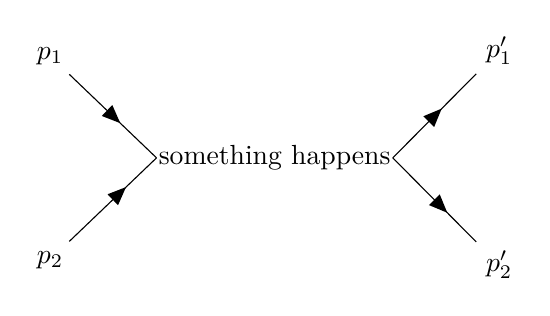
\begin{tikzpicture}
      \begin{feynman}
        \vertex (m1);
        \vertex [above left=of m1] (i1) {$p_1$};
        \vertex [below left=of m1] (i2) {$p_2$};
        \vertex [right=of m1] (mm);
        \vertex [right=of mm] (m2);
        \vertex [above right=of m2] (f1) {$p_1'$};
        \vertex [below right=of m2] (f2) {$p_2'$};

        \node at (mm) {something happens};

        \diagram*{
          (i1) -- [fermion] (m1) -- [anti fermion] (i2),
          (f2) -- [anti fermion] (m2) -- [fermion] (f1),
        };
      \end{feynman}
    \end{tikzpicture}
  \end{center}
  Then we have initial and final states
  \begin{align*}
    \bket{i} &= \sqrt{4 E_{\mathbf{p}_1} E_{\mathbf{p}_2}} b_{\mathbf{p}_1}^\dagger b_{\mathbf{p}_2}^\dagger\bket{0}\\
    \bket{f} &= \sqrt{4 E_{\mathbf{p}_1'} E_{\mathbf{p}_2'}} b_{\mathbf{p}_1'}^\dagger b_{\mathbf{p}_2'}^\dagger\bket{0}
  \end{align*}
  We look at the order $g^2$ term in $\brak{f}(S - \mathbf{1})\bket{i}$. We remove that $\mathbf{1}$ as we are not interested in the case with no scattering, and we look at order $g^2$ because there is no order $g$ term.

  The second order term is given by
  \[
    \frac{(-ig)^2}{2}\int \d^4 x_1 \d^4 x_2 \; T\left[\psi^\dagger(x_1) \psi(x_1) \phi(x_1) \psi^\dagger(x_2) \psi(x_2) \phi(x_2)\right].
  \]
  Now we can use Wick's theorem to write the time-ordered product as a sum of normal-ordered products. The annihilation and creation operators don't end up killing the vacuum only if we annihilate two $b_\mathbf{p}$ and then construct two new $b_\mathbf{p}$. This only happens in the term
  \[
    \normalorder{\psi^\dagger(x_1) \psi(x_1) \psi^\dagger(x_2) \psi(x_2)} \contraction{}{\phi}{(x_1)}{\phi}\phi(x_1)\phi(x_2).
  \]
  We know the contraction is given by the Feynman propagator $\Delta_F(x_1 - x_2)$. So we now want to compute
  \[
    \brak{p_1', p_2'} \normalorder{\psi^\dagger(x_1) \psi(x_1) \psi^\dagger(x_2) \psi(x_2)}\bket{p_1, p_2}
  \]
  The only relevant term in the normal-ordered product is
  \[
    \iiiint \frac{\d^3 \mathbf{k}_1\;\d^3 \mathbf{k}_2 \;\d^3 \mathbf{k}_3 \;\d^3 \mathbf{k}_4}{(2\pi)^{12}\sqrt{16 E_{\mathbf{k}_1} E_{\mathbf{k}_2} E_{\mathbf{k}_3} E_{\mathbf{k}_4}}} b_{\mathbf{k}_1}^\dagger b_{\mathbf{k}_2}^\dagger b_{\mathbf{k}_3} b_{\mathbf{k}_4} e^{ik_1 \cdot x_1 + i k_2 \cdot x_2 - i k_3 \cdot x_1 - i k_4 \cdot x_2}.
  \]
  Now letting this act on $\brak{p_1', p_2'}$ and $\bket{p_1, p_2}$ would then give
  \[
    e^{ix_1 \cdot (p_1' - p_1) + i x_2 \cdot (p_2' - p_2)} + e^{ix_1(p_2' - p_1) + i x_1 (p_1' - p_1)}, \tag{$*$}
  \]
  plus what we get by swapping $x_1$ and $x_2$ by a routine calculation (swap the $b$-operators in the $\psi$ with those that create $\bket{i}, \bket{f}$, insert the delta functions as commutators, then integrate).

  What we really want is to integrate the Hamiltonian. So we want to integrate the result of the above computation with respect to all spacetime to obtain
  \begin{align*}
    &\hphantom{=}\frac{(-ig)^2}{2} \int \d^4 x_1\;\d^4 x_2 \;(*)\; \Delta_F(x_1 - x_2)\\
    &= \frac{(-ig)^2}{2}\int \d^4 x_1\;\d^4 x_2 \;(*)\; \int \frac{\d^4 k}{(2\pi)^4} \frac{e^{ik\cdot(x_1 - x_2)}}{k^2 - m^2 + i \varepsilon}\\
    &=(-ig)^2 \int \frac{\d^4 k}{(2\pi)^4} \frac{i (2\pi)^8}{k^2 - m^2 + i \varepsilon} \\
    &\hphantom{=(-ig)^2 \int}\Big(\delta^4(p_1' - p_1 + k) \delta^4(p_2' - p_2 - k) + \delta^4(p_2' - p_1 + k) \delta^4(p_1' - p_2 - k)\Big)\\
    &= (-ig)^2 (2\pi)^4\left(\frac{i}{(p_1 - p_1')^2 - m^2} + \frac{i}{(p_1 - p_2')^2 - m^2}\right) \delta^4(p_1 + p_2 - p_1' - p_2').
  \end{align*}
  What we see again is a $\delta$-function that enforces momentum conservation.
\end{eg}

\subsection{Feynman diagrams}
This is better, but still rather tedious. How can we make this better? In the previous example, we could imagine that the term that contributed to the integral above represented the interaction where the two $\psi$-particles ``exchanged'' a $\phi$-particle. In this process, we destroy the old $\psi$-particles and construct new ones with new momenta, and the $\phi$-particle is created and then swiftly destroyed. The fact that the $\phi$-particles were just ``intermediate'' corresponds to the fact that we included their contraction in the computation.

We can pictorially represent the interaction as follows:
\begin{center}
  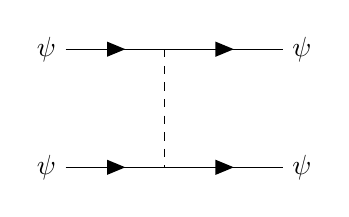
\begin{tikzpicture}
    \begin{feynman}
      \vertex (i1) {$\psi$};
      \vertex [below=of i1] (i2) {$\psi$};

      \vertex [right=of i1] (m1);
      \vertex [right=of m1] (f1) {$\psi$};
      \vertex [right=of i2] (m2);
      \vertex [right=of m2] (f2) {$\psi$};

      \diagram* {
        (i1) -- [fermion] (m1) -- [fermion] (f1),
        (i2) -- [fermion] (m2) -- [fermion] (f2),
        (m1) -- [scalar] (m2),
      };
    \end{feynman}
  \end{tikzpicture}
\end{center}
The magical insight is that \emph{every} term given by Wick's theorem can be interpreted as a diagram of this sort. Moreover, the term contributes to the process if and only if it has the right ``incoming'' and ``outgoing'' particles. So we can figure out what terms contribute by drawing the right diagrams.

Moreover, not only can we count the diagrams like this. More importantly, we can read out how much each term contributes from the diagram directly! This simplifies the computation a lot.

We will not provide a proof that Feynman diagrams do indeed work, as it would be purely technical and would also involve the difficult work of what it actually means to be a diagram. However, based on the computations we've done above, one should be confident that at least something of this sort would work, maybe up to some sign errors.

We begin by specifying what diagrams are ``allowed'', and then specify how we assign numbers to diagrams.

Given an initial state and final state, the possible Feynman diagrams are specified as follows:
\begin{defi}[Feynman diagram]\index{Feynman diagram!scalar Yukawa theory}\index{Feynman diagram}
  In the scalar Yukawa theory, given an initial state $\bket{i}$ and final state $\bket{f}$, a \emph{Feynman diagram} consists of:
  \begin{itemize}
    \item An external line for all particles in the initial and final states. A dashed line is used for a $\phi$-particle, and solid lines are used for $\psi$/$\bar\psi$-particles.
    \begin{center}
      \begin{tikzpicture}
        \begin{feynman}
          \vertex (i) {$\phi$};
          \vertex [right=of i] (b);
          \vertex [above right=of b] (a1);
          \vertex [below right=of b] (a2);

          \vertex [right=of a1] (f1) {$\psi$};
          \vertex [right=of a2] (f2) {$\bar{\psi}$};

          \diagram* {
            (i) -- [scalar] (b),
            (a1) -- (f1),
            (a2) -- (f2),
          };
        \end{feynman}
      \end{tikzpicture}
    \end{center}
  \item Each $\psi$-particle comes with an arrow. An initial $\psi$-particle has an incoming arrow, and a final $\psi$-particle has an outgoing arrow. The reverse is done for $\bar\psi$-particles.
    \begin{center}
      \begin{tikzpicture}
        \begin{feynman}
          \vertex (i) {$\phi$};
          \vertex [right=of i] (b);
          \vertex [above right=of b] (a1);
          \vertex [below right=of b] (a2);

          \vertex [right=of a1] (f1) {$\psi$};
          \vertex [right=of a2] (f2) {$\bar{\psi}$};

          \diagram* {
            (i) -- [scalar] (b),
            (a1) -- [fermion] (f1),
            (a2) -- [anti fermion] (f2),
          };
        \end{feynman}
      \end{tikzpicture}
    \end{center}
  \item We join the lines together with more lines and vertices so that the only loose ends are the initial and final states. The possible vertices correspond to the interaction terms in the Lagrangian. For example, the only interaction term in the Lagrangian here is $\psi^\dagger \psi \phi$, so the only possible vertex is one that joins a $\phi$ line with two $\psi$ lines that point in opposite directions:
    \begin{center}
      \begin{tikzpicture}
        \begin{feynman}
          \vertex (i) {$\phi$};
          \vertex [right=of i] (a);
          \vertex [above right=of a] (f1) {$\psi$};
          \vertex [below right=of a] (f2) {$\bar{\psi}$};

          \diagram* {
            (i) -- [scalar] (a),
            (f1) -- [fermion] (a) -- [fermion] (f2),
          };
        \end{feynman}
      \end{tikzpicture}
    \end{center}
    Each such vertex represents an interaction, and the fact that the arrows match up in all possible interactions ensures that charge is conserved.

    \item Assign a directed momentum $p$ to each line, i.e.\ an arrow into or out of the diagram to each line.
      \begin{center}
        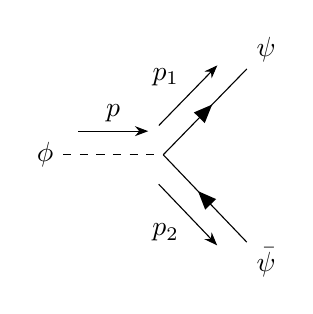
\begin{tikzpicture}
          \begin{feynman}
            \vertex (i) {$\phi$};
            \vertex [right=of i] (a);
            \vertex [above right=of a] (f1) {$\psi$};
            \vertex [below right=of a] (f2) {$\bar{\psi}$};

            \diagram* {
              (i) -- [scalar, momentum=$p$] (a),
              (f2) -- [fermion, reversed momentum=$p_2$] (a) -- [fermion, momentum=$p_1$] (f1),
            };
          \end{feynman}
        \end{tikzpicture}
      \end{center}
      The initial and final particles already have momentum specified in the initial and final state, and the internal lines are given ``dummy'' momenta $k_i$ (which we will later integrate over).
  \end{itemize}
\end{defi}
Note that there are infinitely many possible diagrams! However, when we lay down the Feynman rules later, we will see that the more vertices the diagram has, the less it contributes to the sum. In fact, the $n$-vertices diagrams correspond to the $n$th order term in the expansion of the $S$-matrix. So most of the time it suffices to consider ``simple'' diagrams.

\begin{eg}[Nucleon scattering]
  If we look at $\psi + \psi \to \psi + \psi$, the simplest diagram is
  \begin{center}
    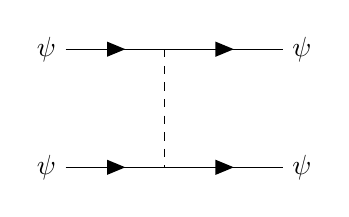
\begin{tikzpicture}
      \begin{feynman}
        \vertex (i1) {$\psi$};
        \vertex [below=of i1] (i2) {$\psi$};

        \vertex [right=of i1] (m1);
        \vertex [right=of m1] (f1) {$\psi$};
        \vertex [right=of i2] (m2);
        \vertex [right=of m2] (f2) {$\psi$};

        \diagram* {
          (i1) -- [fermion] (m1) -- [fermion] (f1),
          (i2) -- [fermion] (m2) -- [fermion] (f2),
          (m1) -- [scalar] (m2),
        };
      \end{feynman}
    \end{tikzpicture}
  \end{center}
  On the other hand, we can also swap the two particles to obtain a diagram of the form.
  \begin{center}
    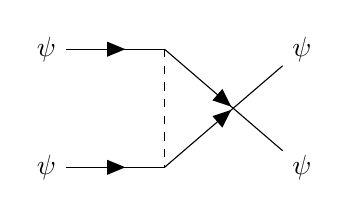
\begin{tikzpicture}
      \begin{feynman}
        \vertex (i1) {$\psi$};
        \vertex [below=of i1] (i2) {$\psi$};

        \vertex [right=of i1] (m1);
        \vertex [right=of m1] (f1) {$\psi$};
        \vertex [right=of i2] (m2);
        \vertex [right=of m2] (f2) {$\psi$};

        \diagram* {
          (i1) -- [fermion] (m1) -- [fermion] (f2),
          (i2) -- [fermion] (m2) -- [fermion] (f1),
          (m1) -- [scalar] (m2),
        };
      \end{feynman}
    \end{tikzpicture}
  \end{center}
  These are the ones that correspond to second-order terms.

  There are also more complicated ones such as
  \begin{center}
    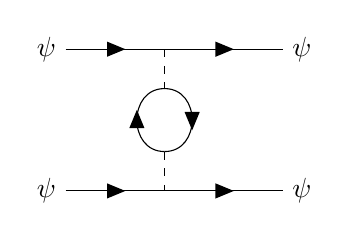
\begin{tikzpicture}
      \begin{feynman}
        \vertex (i1) {$\psi$};
        \vertex [below=1.8cm of i1] (i2) {$\psi$};

        \vertex [right=of i1] (m1);
        \vertex [right=of m1] (f1) {$\psi$};
        \vertex [right=of i2] (m2);
        \vertex [right=of m2] (f2) {$\psi$};

        \vertex [below=0.5cm of m1] (c1);
        \vertex [below=0.8cm of c1] (c2);

        \diagram* {
          (i1) -- [fermion] (m1) -- [fermion] (f1),
          (i2) -- [fermion] (m2) -- [fermion] (f2),
          (m1) -- [scalar] (c1) -- [fermion, half left] (c2) -- [fermion, half left] (c1),
          (c2) -- [scalar] (m2),
        };
      \end{feynman}
    \end{tikzpicture}
  \end{center}
  This is a \term{1-loop diagram}. We can also have a \term{2-loop diagram}:
  \begin{center}
    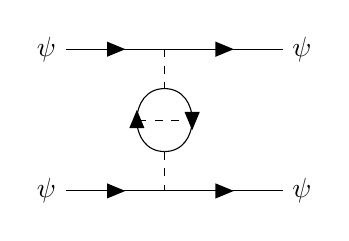
\begin{tikzpicture}
      \begin{feynman}
        \vertex (i1) {$\psi$};
        \vertex [below=1.8cm of i1] (i2) {$\psi$};

        \vertex [right=of i1] (m1);
        \vertex [right=of m1] (f1) {$\psi$};
        \vertex [right=of i2] (m2);
        \vertex [right=of m2] (f2) {$\psi$};

        \vertex [below=0.5cm of m1] (c1);
        \vertex [below=0.8cm of c1] (c2);

        \vertex [below right=0.4cm and 0.4cm of c1] (r);
        \vertex [below left=0.4cm and 0.4cm of c1] (l);
        \diagram* {
          (i1) -- [fermion] (m1) -- [fermion] (f1),
          (i2) -- [fermion] (m2) -- [fermion] (f2),
          (m1) -- [scalar] (c1) -- [fermion, half left] (c2) -- [fermion, half left] (c1),
          (c2) -- [scalar] (m2),
          (r) -- [scalar] (l),
        };
      \end{feynman}
    \end{tikzpicture}
  \end{center}
  If we ignore the loops, we say we are looking at the \term{tree level}.
\end{eg}

To each such diagram, we associate a number using the \emph{Feynman rules}.
\begin{defi}[Feynman rules]\index{Feynman rules}
  To each Feynman diagram in the interaction, we write down a term like this:
  \begin{enumerate}
    \item To each vertex in the Feynman diagram, we write a factor of
      \[
        (-ig)(2\pi)^4 \delta^4\left(\sum_i k_i\right),
      \]
      where the sum goes through all lines going into the vertex (and put a negative sign for those going out).
    \item For each internal line with momentum $k$, we integrate the product of all factors above by
      \[
        \int \frac{\d^4 k}{(2\pi)^4} D(k^2),
      \]
      where
      \begin{align*}
        D(k^2) &= \frac{i}{k^2 - m^2 + i\varepsilon}\text{ for }\phi\\
        D(k^2) &= \frac{i}{k^2 - \mu^2 + i\varepsilon}\text{ for }\psi
      \end{align*}
  \end{enumerate}
\end{defi}

\begin{eg}
  We consider the case where $g$ is small. Then only the simple diagrams with very few vertices matter.
  \begin{center}
    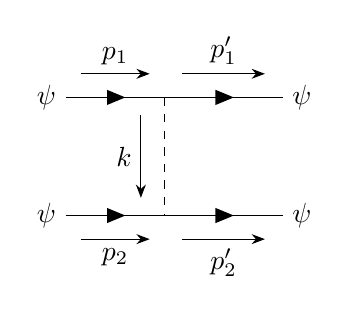
\begin{tikzpicture}
      \begin{feynman}
        \vertex (i1) {$\psi$};
        \vertex [below=of i1] (i2) {$\psi$};

        \vertex [right=of i1] (m1);
        \vertex [right=of m1] (f1) {$\psi$};
        \vertex [right=of i2] (m2);
        \vertex [right=of m2] (f2) {$\psi$};

        \diagram* {
          (i1) -- [fermion, momentum=$p_1$] (m1) -- [fermion, momentum=$p_1'$] (f1),
          (i2) -- [fermion, momentum'=$p_2$] (m2) -- [fermion, momentum'=$p_2'$] (f2),
          (m1) -- [scalar, momentum'=$k$] (m2),
        };
      \end{feynman}
    \end{tikzpicture}
    \quad
    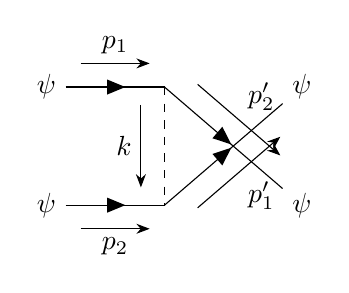
\begin{tikzpicture}
      \begin{feynman}
        \vertex (i1) {$\psi$};
        \vertex [below=of i1] (i2) {$\psi$};

        \vertex [right=of i1] (m1);
        \vertex [right=of m1] (f1) {$\psi$};
        \vertex [right=of i2] (m2);
        \vertex [right=of m2] (f2) {$\psi$};

        \diagram* {
          (i1) -- [fermion, momentum=$p_1$] (m1) -- [fermion, momentum=$p_2'$] (f2),
          (i2) -- [fermion, momentum'=$p_2$] (m2) -- [fermion, momentum'=$p_1'$] (f1),
          (m1) -- [scalar, momentum'=$k$] (m2),
        };
      \end{feynman}
    \end{tikzpicture}
  \end{center}
  As promised by the Feynman rules, the two diagrams give us
  \[
    (-ig)^2 (2\pi)^8(\delta^4(p_1 - p_1' - k) \delta^4(p_2 + k - p_2') + \delta^4(p_1 - p_2' - k)\delta^4(p_2 + k - p_1')).
  \]
  Now integrating gives us the formula
  \begin{multline*}
    (-ig)^2 \int \frac{\d^4 k}{(2\pi)^4} \frac{i(2\pi)^8}{k^2 - m^2 + i \varepsilon}\\
    (\delta^4(p_1 - p_1' - k) \delta^4(p_2 + k - p_2')+ \delta^4(p_1 - p_2' - k)\delta^4(p_2 + k - p_1')).
  \end{multline*}
  Doing the integral gives us
  \[
    (-ig)^2 (2\pi)^4\left(\frac{i}{(p_1 - p_1')^2 - m^2} + \frac{i}{(p_1 - p_2')^2 - m^2}\right) \delta^4(p_1 + p_2 - p_1' - p_2'),
  \]
  which is what we found before.
\end{eg}
There is a nice physical interpretation of the diagrams. We can interpret the first diagram as saying that the nucleons exchange a meson of momentum $k = p_1 - p_1' = p_2 - p_2'$. This meson doesn't necessarily satisfy the relativistic dispersion relation $k^2 = m^2$ (note that $k$ is the $4$-momentum). When this happens, we say it is \term{off-shell}, or that it is a \term{virtual meson}. Heuristically, it can't live long enough for its energy to be measured accurately. In contrast, the external legs are \term{on-shell}, so they satisfy $p_i^2 = \mu^2$.

\subsection{Amplitudes}
Now the important question is --- what do we do with that quantity we computed? We first define a more useful quantity known as the \emph{amplitude}:
\begin{defi}[Amplitude]\index{amplitude}
  The \emph{amplitude} $\mathcal{A}_{f,i}$ of a scattering process from $\bket{i}$ to $\bket{f}$ is defined by
  \[
    \brak{f}S - \mathbf{1}\bket{i} = i \mathcal{A}_{f,i} (2\pi)^4 \delta^4 (p_F - p_I).
  \]
  where $p_F$ is the sum of final state $4$-momenta, and $p_I$ is the sum of initial state $4$-momenta. The factor of $i$ sticking out is by convention, to match with non-relativistic quantum mechanics.
\end{defi}

We can now modify our Feynman rules accordingly to compute $\mathcal{A}_{f, i}$.

\begin{itemize}
  \item Draw all possible diagrams with the appropriate external legs and impose $4$-momentum conservation at each vertex.
  \item Write a factor $(-ig)$ for each vertex.
  \item For each internal line of momentum $p$ and mass $m$, put in a factor of
    \[
      \frac{1}{p^2 - m^2 + i \varepsilon}.
    \]
  \item Integrate over all undetermined $4$-momentum $k$ flowing in each loop.
\end{itemize}

We again do some examples of computation.
\begin{eg}[Nucleon-antinucleon scattering]
  Consider another tree-level process
  \[
    \psi + \bar{\psi} \to \phi + \phi.
  \]
  We have a diagram of the form
  \begin{center}
    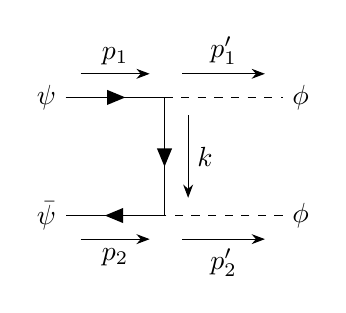
\begin{tikzpicture}
      \begin{feynman}
        \vertex (i1) {$\psi$};
        \vertex [below=of i1] (i2) {$\bar{\psi}$};

        \vertex [right=of i1] (m1);
        \vertex [right=of m1] (f1) {$\phi$};
        \vertex [right=of i2] (m2);
        \vertex [right=of m2] (f2) {$\phi$};

        \diagram* {
          (i1) -- [fermion, momentum=$p_1$] (m1) -- [scalar, momentum=$p_1'$] (f1),
          (f2) -- [scalar, rmomentum=$p_2'$] (m2) -- [fermion, rmomentum=$p_2$] (i2),
          (m1) -- [fermion, momentum=$k$] (m2),
        };
      \end{feynman}
    \end{tikzpicture}
  \end{center}
  and a similar one with the two $\phi$ particles crossing.

  The two diagrams then say
  \[
    \mathcal{A} = (-ig)^2 \left(\frac{1}{(p_1 - p_1')^2 - \mu^2} + \frac{1}{(p_2 - p_2')^2 - \mu^2}\right).
  \]
  Note that we dropped the $i\varepsilon$ terms in the denominator because the denominator never vanishes, and we don't need to integrate over anything because all momenta in the diagram are determined uniquely by momentum conservation.
\end{eg}

\begin{eg}[Meson scattering]
  Consider
  \[
    \phi + \phi \to \phi + \phi.
  \]
  This is a bit more tricky. There is no tree-level diagram we can draw. The best we can get is a box diagram like this:
  \begin{center}
    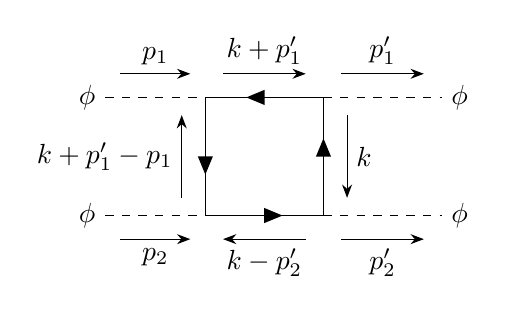
\begin{tikzpicture}
      \begin{feynman}
        \vertex (i1) {$\phi$};
        \vertex [below=of i1] (i2) {$\phi$};

        \vertex [right=of i1] (m1);
        \vertex [right=of m1] (n1);
        \vertex [right=of n1] (f1) {$\phi$};
        \vertex [right=of i2] (m2);
        \vertex [right=of m2] (n2);
        \vertex [right=of n2] (f2) {$\phi$};

        \diagram* {
          (i1) -- [scalar, momentum=$p_1$] (m1),
          (i2) -- [scalar, momentum'=$p_2$] (m2),
          (n1) -- [scalar, momentum=$p_1'$] (f1),
          (n2) -- [scalar, momentum'=$p_2'$] (f2),

          (n1) -- [anti fermion, momentum=$k$] (n2) -- [anti fermion, momentum=$k - p_2'$] (m2) -- [anti fermion, momentum=$k + p_1' - p_1$] (m1) -- [anti fermion, momentum=$k + p_1'$] (n1);
        };
      \end{feynman}
    \end{tikzpicture}
  \end{center}
  We then integrate through all possible $k$.

  This particular graph we've written down gives
  \begin{multline*}
    i\mathcal{A} = (-ig)^4 \int \frac{\d^4 k}{(2\pi)^4}\\\frac{i^4}{(k^2 - \mu^2 + i\varepsilon)((k + p_1')^2 - \mu^2 + i\varepsilon)((k + p_1' - p_1)^2 - \mu^2 + i \varepsilon)((k - p_2')^2 - \mu^2 + i \varepsilon)}.
  \end{multline*}
  For large $k$, this asymptotically tends to $\int \frac{\d^4 k}{k^8}$, which fortunately means the integral converges. However, this is usually not the case. For example, we might have $\frac{\d^4k}{k^4}$, which diverges, or even $\int \frac{\d^4 k}{k^2}$. This is when we need to do renormalization.
\end{eg}

\begin{eg}[Feynman rules for $\phi^4$ theory]
  Suppose our Lagrangian has a term
  \[
    \frac{\lambda}{4!} \phi^4.
  \]
  We then have single-vertex interactions
  \begin{center}
    \begin{tikzpicture}
      \begin{feynman}
        \vertex (c);
        \vertex [above right=of c] (1);
        \vertex [above left=of c] (2);
        \vertex [below right=of c] (3);
        \vertex [below left=of c] (4);
        \diagram* {
          (1) -- [scalar] (c),
          (2) -- [scalar] (c),
          (3) -- [scalar] (c),
          (4) -- [scalar] (c),
        };
      \end{feynman}
    \end{tikzpicture}
  \end{center}
  Any such diagram contributes a factor of $(-i\lambda)$. Note that there is no $\frac{1}{4!}$. This is because if we expand the term
  \[
    \frac{-i \lambda}{4!} \brak{p_1', p_2'} \normalorder{\phi(x_1)\phi(x_2)\phi(x_3)\phi(x_4)}\bket{p_1, p_2},
  \]
  there are $4!$ ways of pairing the $\phi(x_i)$ with the $p_i, p_i'$, so each possible interaction is counted $4!$ times, and cancels that $4!$ factor.

  For some diagrams, there are extra combinatoric factors, known as \term{symmetry factors}, that one must take into account.
\end{eg}

These amplitudes can be further related to experimentally measurable quantities. We will not go into details here, but in The Standard Model course, we will see that if we have a single initial state $i$ and a collection of final states $\{f\}$, then the decay rate of $i$ to $\{f\}$ is given by
\[
  \Gamma_{i \to f} = \frac{1}{2 m_i} \int |\mathcal{A}_{f,i}|^2 \;\d \rho_f,
\]
where
\[
  \d \rho_f = (2\pi)^4 \delta^4(p_F - p_I) \prod_r \frac{\d^3 p_r}{(2\pi)^3 2 p_r^0},
\]
and $r$ runs over all momenta in the final states.

%Now what do we do with the resulting expression? We start by writing down what we think should be the probability of transitioning from $\bket{i}$ to $\bket{f}$:
%\[
% P = \frac{|\brak{f}S - \mathbf{1}\bket{i}|^2}{\braket{f}{f} \braket{i}{i}}.
%\]
%Recall that the terms are given by
%\begin{align*}
% |\brak{f}S- \mathbf{1}\bket{i}|^2 &= |\mathcal{A}_{f, i}| (2\pi)^8 (\delta^4(p_F - p_I))^2\\
% &= |\mathcal{A}_{f, i}| (2\pi)^8 \delta^4(p_F - p_I) \delta^4(0)\\
% \braket{i}{i} &= \prod_{\text{initial particles}} (2\pi)^3 2 E_{\mathbf{p}_i} \delta^3(0)\\
% \braket{f}{f} &= \prod_{\text{final particles}} (2\pi)^3 2 E_{\mathbf{p}_i} \delta^3(0)
%\end{align*}
%So we found that
%\[
% P \qeq |\mathcal{A}_{f, i}| (2\pi)^8 \delta^4(p_F - p_I) \delta^4(0)\prod_{\text{all particles}} \frac{1}{(2\pi)^3 2E_{\mathbf{p}_i}\delta^3(0)}.
%\]
%We again have a lot of scary $\delta$-functions. As before, if we trace through the calculations, we will find that $(2\pi)^3\delta^3(0)$ comes from integrating over the volume of the whole universe, so we use the trick of replacing $(2\pi)^3\delta^3(0)$ with the volume $V$ of the universe. Similarly, $(2\pi)^4\delta^4(0)$ is the total spacetime volume of the universe $VT$.
%
%So we have a slightly better expression
%\[
% |\mathcal{A}_{f, i}|^2 (2\pi)^4 \delta^4(p_F - p_I) VT \prod_{\text{all particles}} \frac{1}{2E_{\mathbf{p}_i} V}.
%\]
%Remember that all the $V$ and $T$ will be taken to be infinity eventually. So we would like to get rid of them. Here we can easily get rid of the $T$, because we can instead ask for the probability of decaying to $\bket{f}$ in \emph{unit time}. So we are left with
%\[
% |\mathcal{A}_{f, i}|^2 (2\pi)^4 \delta^4(p_F - p_I) V \prod_{\text{all particles}} \frac{1}{2E_{\mathbf{p}_i} V}.
%\]
%What do we do next? We are computing the probability of transitioning from $\bket{i}$ to exactly $\bket{f}$. As one might expect, since the momentum has a continuous range of values, it is virtually impossible to obtain exactly $\bket{f}$. Instead, a more sensible question might be to ask the probability of decaying into, say, two $\psi$ particles, and then we integrate the above expression over all conceivable pairs of momenta. We might want to just integrate against
%\[
% \d \Pi = \prod_{i \text{ final}}\d^3 \mathbf{p}_i,
%\]
%but this is not the right thing to integrate over, because $\int \d \Pi \not= 1$. Instead, the correctly noramlized version is
%\[
% \d \Pi = \prod_{i \text{ final}} \frac{V \d^3 \mathbf{p}_i}{(2\pi)^3}.
%\]
%I have not yet figured out how this can be made to work, actually. This was not done in lectures and explanations I have found seem unsatisfactory.

%We can take our quantum calculations of the $\psi \psi \to \psi \psi$ and take a classical limit. This then gives us a potential for the interaction of two $\psi$ particles, given by
%\[
% U(r) = -\frac{\lambda^2 e^{-mr}}{4 \pi r}.
%\]
%Here
%\[
% \lambda = \frac{g}{2\mu},
%\]
%where the $2\mu$ comes from non-relativistic normalization. The negative sign tells us the force is attractive.
%
%We can do exactly the same calculation for nucleon-antinucleon scattering, which also gives an attractive force. In general, the exchange of scalar fields gives us an attractive force. When spin $1$ particles are being exchanged, we get attractive forces for like particles, and repulsive forces for unlike particles. When we get up to spin $2$ particles, everything is again attractive, and this can be used to model gravity. There are more details on David Tong's notes.
%
%Note that for the $\phi^4$, theory, we have
%\[
% i\mathcal{A} = -i \lambda.
%\]
%So we have
%\[
% U(\mathbf{r}) = - \lambda \int \frac{\d^3 \mathbf{p}}{(2\pi)^3} e^{i\mathbf{p}\cdot \mathbf{r}} = -\lambda \delta^3 \mathbf{r}.
%\]
\subsection{Correlation functions and vacuum bubbles}
The $S$-matrix elements are good and physical, because they correspond to probabilities of certain events happening. However, we are not always interested in these quantities. For example, we might want to ask the conductivity of some quantum-field-theoretic object. To do these computations, quantities known as \emph{correlation functions} are useful. However, we are not going to use these objects in this course, so we are just going to state, rather than justify many of the results, and you are free to skip this chapter.

Before that, we need to study the vacuum. Previously, we have been working with the vacuum of the free theory $\bket{0}$. This satisfies the boring relation
\[
  H_0 \bket{0} = 0.
\]
However, when we introduce an interaction term, this is no longer the vacuum. Instead we have an interacting vacuum $\bket{\Omega}$, satisfying
\[
  H \bket{\Omega} = 0.
\]
As before, we normalize the vacuum so that
\[
  \braket{\Omega}{\Omega} = 1.
\]
Concretely, this interaction vacuum can be obtained by starting with a free vacuum and then letting it evolve for infinite time.
\begin{lemma}
  The free vacuum and interacting vacuum are related via
  \[
    \bket{\Omega} = \frac{1}{\braket{\Omega}{0}} U_I(t, -\infty)\bket{0} = \frac{1}{\braket{\Omega}{0}} U_S(t, -\infty)\bket{0}.
  \]
Similarly, we have
  \[
    \brak{\Omega} = \frac{1}{\braket{\Omega}{0}} \brak{0}U(\infty, t).
  \]
\end{lemma}

\begin{proof}
  Note that we have the last equality because $U_I(t, -\infty)$ and $U_S(t, -\infty)$ differs by factors of $e^{-iH t_0}$ which acts as the identity on $\bket{0}$. % I am not convinced.

  Consider an arbitrary state $\bket{\Psi}$. We want to show that
  \[
    \brak{\Psi}U(t, -\infty)\bket{0} = \braket{\Psi}{\Omega}\braket{\Omega}{0}.
  \]
  The trick is to consider a complete set of eigenstates $\{\Omega, \bket{x}\}$ for $H$ with energies $E_x$. Then we have
  \[
    U(t, t_0) \bket{x} = e^{iE_x(t_0 - t)} \bket{x}.
  \]
  Also, we know that
  \[
    \mathbf{1} = \bket{\Omega}\brak{\Omega} + \int \d x\; \bket{x}\brak{x}.
  \]
  So we have
  \begin{align*}
    \brak{\Psi}U(t, -\infty) \bket{0} &= \brak{\Psi}U(t, -\infty) \left(\bket{\Omega}\brak{\Omega} + \int \;\d x \bket{x}\brak{x}\right)\bket{0}\\
    &= \braket{\Psi}{\Omega} \braket{\Omega}{0} + \lim_{t' \to -\infty} \int\d x\; e^{iE_x(t' - t)} \braket{\Psi}{x} \braket{x}{0}.
  \end{align*}
  We now claim that the second term vanishes in the limit. As in most of the things in the course, we do not have a rigorous justification for this, but it is not too far-stretched to say so since for any well-behaved (genuine) function $f(x)$, the \emph{Riemann-Lebesgue lemma} tells us that for any fixed $a, b \in \R$, we have
  \[
    \lim_{\mu \to \infty} \int_a^b f(x) e^{i\mu x}\;\d x = 0.
  \]
  If this were to hold, then
  \[
    \brak{\Psi}U(t, -\infty)\bket{0} = \braket{\Psi}{\Omega}\braket{\Omega}{0}.
  \]
  So the result follows. The other direction follows similarly.
\end{proof}

Now given that we have this vacuum, we can define the \emph{correlation function}.
\begin{defi}[Correlation/Green's function]\index{correlation function}\index{Green's function}
  The \emph{correlation} or \emph{Green's function} is defined as
  \[
    G^{(n)}(x_1, \cdots, x_n) = \brak{\Omega}T \phi_H(x_1) \cdots \phi_H(x_n)\bket{\Omega},
  \]
  where $\phi_H$ denotes the operators in the Heisenberg picture.
\end{defi}

How can we compute these things? We claim the following:
\begin{prop}
  \[
    G^{(n)}(x_1, \cdots, x_n) = \frac{\brak{0}T \phi_I(x_1) \cdots \phi_I(x_n)S \bket{0}}{\brak{0}S\bket{0}}.
  \]
\end{prop}

\begin{proof}
  We can wlog consider the specific example $t_1 > t_2 > \cdots > t_n$. We start by working on the denominator. We have
  \[
    \brak{0}S\bket{0} = \brak{0}U(\infty, t) U(t, -\infty)\bket{0} = \braket{0}{\Omega}\braket{\Omega}{\Omega}\braket{\Omega}{0}.
  \]
  For the numerator, we note that $S$ can be written as
  \[
    S = U_I(\infty, t_1) U_I(t_1, t_2) \cdots U_I(t_n, -\infty).
  \]
  So after time-ordering, we know the numerator of the right hand side is
  \[
    \brak{0}U_I(\infty, t_1) \phi_I(x_1) U_I(t_1, t_2) \phi_I(x_2) \cdots \phi_I(n)U_I(t_n, -\infty)\bket{0}
  \]
  \begin{align*}
    &\hphantom{=}\brak{0}U_I(\infty, t_1) \phi_I(x_1) U_I(t_1, t_2) \phi_I(x_2) \cdots \phi_I(n)U_I(t_n, -\infty)\bket{0}\\
    &=\brak{0}U_I(\infty, t_1) \phi_H(x_1) \cdots \phi_H(x_n) U_I(t_n, -\infty)\bket{0}\\
    &=\braket{0}{\Omega}\brak{\Omega}T \phi_H(x_1) \cdots \phi_H(x_n)\bket{\Omega}\braket{\Omega}{0}.
  \end{align*}
  So the result follows. % why can we convert like that?
\end{proof}

Now what does this quantity tell us? It turns out these have some really nice physical interpretation. Let's look at the terms $\brak{0}T \phi_I(x_1) \cdots \phi_I(x_n) S \bket{0}$ and $\brak{0}S\bket{0}$ individually and see what they tell us.

For simplicity, we will work with the $\phi^4$ theory, so that we only have a single $\phi$ field, and we will, without risk of confusion, draw all diagrams with solid lines.

Looking at $\brak{0}S\bket{0}$, we are looking at all transitions from $\bket{0}$ to $\bket{0}$. The Feynman diagrams corresponding to these would look like
\begin{center}
  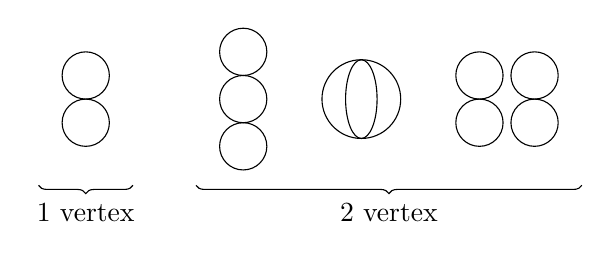
\begin{tikzpicture}
    \draw (2, 0.3) circle [radius=0.3];
    \draw (2, -0.3) circle [radius=0.3];

    \draw (4, 0.6) circle [radius=0.3];
    \draw (4, 0) circle [radius=0.3];
    \draw (4, -0.6) circle [radius=0.3];

    \draw (5.5, 0) circle [radius=0.5];
    \draw (5.5, 0) ellipse (0.2 and 0.5);

    \draw (7, 0.3) circle [radius=0.3];
    \draw (7, -0.3) circle [radius=0.3];
    \draw (7.7, 0.3) circle [radius=0.3];
    \draw (7.7, -0.3) circle [radius=0.3];

    \draw [decorate, decoration={brace, amplitude=3pt, raise=-3pt}] (2.6, -1.2) -- (1.4, -1.2) node [pos=0.5, below] {$1$ vertex};
    \draw [decorate, decoration={brace, amplitude=3pt, raise=-3pt}] (8.3, -1.2) -- (3.4, -1.2) node [pos=0.5, below] {$2$ vertex};
  \end{tikzpicture}
\end{center}
These are known as vacuum bubbles. Then $\brak{0}S\bket{0}$ is the sum of the amplitudes of all these vacuum bubbles.

While this sounds complicated, a miracle occurs. It happens that the different combinatoric factors piece together nicely so that we have
\[
  \brak{0}S \bket{0} = \exp(\text{all distinct (connected) vacuum bubbles}).
\]
Similarly, magic tells us that
\[
  \brak{0}T\phi_I(x_1) \cdots \phi_I(x_n) S \bket{0} =\left(\sum \parbox{9em}{connected diagrams with $n$ loose ends}\right) \brak{0}S\bket{0}.
\]
So what $G^{(n)}(x_1, \cdots, x_n)$ really tells us is the sum of connected diagrams modulo these silly vacuum bubbles.

\begin{eg}
  The diagrams that correspond to $G^{(4)}(x_1, \cdots, x_4)$ include things that look like
  \begin{center}
    \begin{tikzpicture}
      \draw (0, 0) node [left] {$x_1$} node [circ] {} -- (1, 0) node [circ] {} node [right] {$x_2$};
      \draw (0, -1) node [left] {$x_3$} node [circ] {} -- (1, -1) node [circ] {} node [right] {$x_4$};

      \draw (3, 0) node [left] {$x_1$} node [circ] {} -- (4, -1) node [circ] {} node [right] {$x_4$};
      \draw (3, -1) node [left] {$x_3$} node [circ] {} -- (4, 0) node [circ] {} node [right] {$x_2$};

      \draw (6, 0) node [left] {$x_1$} node [circ] {} -- (7, 0) node [circ] {} node [right] {$x_2$};
      \draw (6, -1) node [left] {$x_3$} node [circ] {} -- (6.5, -0.7) -- (7, -1) node [circ] {} node [right] {$x_4$};
      \draw (6.5, -0.5) circle [radius=0.2];
    \end{tikzpicture}
  \end{center}
  Note that we define ``connected'' to mean every line is connected to some of the end points in some way, rather than everything being connected to everything.
\end{eg}
We can come up with analogous Feynman rules to figure out the contribution of all of these terms.

%For scalar Yukawa theory, the vacuum bubbles may look like these:
%\begin{center}
% \begin{tikzpicture}
% \begin{feynman}
% \vertex (r);
% \vertex [right=of r] (l);
%
% \diagram*{
% (r) -- [fermion, half right] (l) -- [fermion, half right] (r),
% (r) -- [scalar] (l),
% };
% \end{feynman}
% \end{tikzpicture}
% \quad
% \begin{tikzpicture}
% \begin{feynman}
% \vertex (r);
% \vertex [right=of r] (l);
%
% \vertex [right=of l] (r');
% \vertex [right=of r'] (l');
%
% \diagram*{
% (r) -- [fermion, half right] (l) -- [fermion, half right] (r),
% (r') -- [fermion, half right] (l') -- [fermion, half right] (r'),
% (l) -- [scalar] (r'),
% };
% \end{feynman}
% \end{tikzpicture}
%\end{center}
%With a little thought, we can show that
%Here connected means that every point in the diagram is connected to at least $1$ external le.g.\ For example, the following are connected:
%\begin{center}
% \begin{tikzpicture}
% \begin{feynman}
% \vertex (l);
% \vertex [right=of l] (r);
% \diagram*{
% (l) -- [scalar] (r),
% };
% \end{feynman}
% \end{tikzpicture}
% \begin{tikzpicture}
% \begin{feynman}
% \vertex (l);
% \vertex [right=of l] (m);
% \vertex [right=of m] (r);
% \vertex [above=of m] (t);
%
% \diagram*{
% (l) -- [scalar] (m) -- [scalar] (r),
% (m) -- [scalar, half left] (t) -- [scalar, half left] (m),
% };
% \end{feynman}
% \end{tikzpicture}
%\end{center}
%So we learn that
%\[
% \brak{\Omega}T \phi_H(x_1), \cdots, \phi_H(x_n)\bket{\Omega} = \sum\text{connected Feynman diagrams}.
%\]
%Here the Feynman diagrams depend on $x_i$, whereas in the $S$-matrix we integrated them.
%
%It is simple to adopt the Feynman rules for momentum space to compute $G^{(n)}(x_1, \cdots, x_n)$ directly. We simply draw $n$ external points $x_1, \cdots, x_n$. We connect them with propagators (i.e.\ lines), and vertices.
%
%For example, to compute $\brak{\Omega} T \phi_H(x_1) \cdots \phi_H(x_4) \bket{\Omega}$, we have the $0$th order terms
%\begin{center}
% \begin{tikzpicture}
% \begin{feynman}
% \vertex (tl);
% \vertex [right=of tl] (tr);
% \vertex [below=of tl] (bl);
% \vertex [right=of bl] (br);
% \diagram* {
% (tl) -- [scalar] (tr),
% (bl) -- [scalar] (br),
% };
% \end{feynman}
% \end{tikzpicture}
%\end{center}
%and similarly $3$ other diagrams that connect the dots. We then have higher order terms like
%\begin{center}
% \begin{tikzpicture}
% \begin{feynman}
% \vertex (tl);
% \vertex [right=1.5cm of tl] (tr);
% \vertex [below=1.5cm of tl] (bl);
% \vertex [right=1.5cm of bl] (br);
% \vertex [right=0.75cm of bl] (bm);
% \vertex [above=0.75cm of bm] (bb);
% \diagram* {
% (tl) -- [scalar] (tr),
% (bl) -- [scalar] (br),
% (bm) -- [scalar, half left] (bb) -- [scalar, half left] (bm),
% };
% \end{feynman}
% \end{tikzpicture}
%\end{center}
%Green's functions are a handy tool to describe scattering because they avoid the previous complications.

There is also another way we can think about these Green's function. Consider the theory with a source $J(x)$ added, so that
\[
  H = H_0 + H_{\mathrm{int}} - J(x) \phi(x).
\]
This $J$ is a fixed background function, called a source in analogy with electromagnetism.

Consider the interaction picture, but now we choose $(H_0 + H_{\mathrm{int}})$ to be the ``free'' part, and $-J \phi$ as the ``interaction'' piece.

Now the ``vacuum'' we use is not $\bket{0}$ but $\bket{\Omega}$, since this is the ``free vacuum'' for our theory.
We define
\[
  W[J] = \brak{\Omega}U_I(-\infty, \infty) \bket{\Omega}.
\]
This is then a functional in $J$. We can compute
\begin{align*}
  W[J] &= \brak{\Omega}U_I(-\infty, \infty) \bket{\Omega}\\
  &= \brak{\Omega} T \exp\left(\int \d^4 x\; -J(x) \phi_H(x)\right)\bket{\Omega}\\
  &= 1 + \sum_{n = 1}^\infty \frac{(-1)^n}{n!} \int \d^4 x_1 \cdots \d^4 x_n \; J(x_1) \cdots J(x_n) G^{(n)}(x_1, \cdots, x_n).
\end{align*}
Thus by general variational calculus, we know
\[
  G^{(n)}(x_1, \cdots, x_n) = (-1)^n \left.\frac{\delta^n W[J]}{\delta J(x_1) \cdots \delta J(x_n)} \right|_{J = 0}.
\]
Thus we call $W[J]$ a \emph{generating function} for the function $G^{(n)}(x_1, \cdots, x_n)$.

%We can compute $W[J]$ by using the rules prescribed earlier, amended to include the vertex including the source $iJ(x)$. Often, one first defines a related generating function
%\[
% Z[J] = \brak{0}S\bket{0}
%\]
%which sums over all Feynman diagrams, and order $n$, is given by
%\[
% Z[J] = e^{W[J]}.
%\]
%Here $W([J]$ sums over all connected diagrams.

\section{Spinors}
In this chapter, we return to the classical world where things make sense. We are going to come up with the notion of a \emph{spinor}, which is a special type of field that, when quantized, gives us particles with ``intrinsic spin''.

\subsection{The Lorentz group and the Lorentz algebra}
So far, we have only been working with scalar fields. These are pretty boring, since when we change coordinates, the values of the field remain unchanged. One can certainly imagine more exciting fields, like the electromagnetic potential. Ignoring issues of choice of gauge, we can imagine the electromagnetic potential as a $4$-vector $A^\mu$ at each point in space-time. When we change coordinates by a Lorentz transformation $\Lambda$, the field transforms by
\[
  A^\mu(x) \mapsto \Lambda^\mu\!_\nu A^\nu(\Lambda^{-1} x).
\]
Note that we had to put a $\Lambda^{-1}$ inside $A^\nu$ because the names of the points have changed. $\Lambda^{-1}x$ in the new coordinate system labels the same point as $x$ in the old coordinate system.

In general, we can consider vector-valued fields that transform when we change coordinates. If we were to construct such a field, then given any Lorentz transformation $\Lambda$, we need to produce a corresponding transformation $D(\Lambda)$ of the field. If our field $\phi$ takes values in a vector space $V$ (usually $\R^n$), then this $D(\Lambda)$ should be a linear map $V \to V$. The transformation rule is then
\begin{align*}
  x &\mapsto \Lambda x,\\
  \phi &\mapsto D(\Lambda) \phi.
\end{align*}
We want to be sure this assignment of $D(\Lambda)$ behaves sensibly. For example, if we apply the Lorentz transformation $\Lambda = \mathbf{1}$, i.e.\ we do nothing, then $D(\mathbf{1})$ should not do anything as well. So we must have
\[
  D(\mathbf{1}) = \mathbf{1}.
\]
Now if we do $\Lambda_1$ and then $\Lambda_2$, then our field will transform first by $D(\Lambda_1)$, then $D(\Lambda_2)$. For the universe to make sense, this had better be equal to $D(\Lambda_2 \Lambda_1)$. So we require
\[
  D(\Lambda_1)D(\Lambda_2) = D(\Lambda_1 \Lambda_2)
\]
for any $\Lambda_1, \Lambda_2$. Mathematically, we call this a \emph{representation of the Lorentz group}.
\begin{defi}[Lorentz group]\index{Lorentz group}\index{$\Or(1, 3)$}
  The \emph{Lorentz group}, denoted $\Or(1, 3)$, is the group of all Lorentz transformations. Explicitly, it is given by
  \[
    \Or(1, 3) = \{\Lambda \in M_{4\times 4}: \Lambda^T \eta \Lambda = \eta\},
  \]
  where
  \[
    \eta = \eta_{\mu\nu} =
    \begin{pmatrix}
      1 & 0 & 0 & 0\\
      0 & -1 & 0 & 0\\
      0 & 0 & -1 & 0\\
      0 & 0 & 0 & -1
    \end{pmatrix}
  \]
  is the \term{Minkowski metric}. Alternatively, $\Or(1, 3)$ is the group of all matrices $\Lambda$ such that
  \[
    \bra \Lambda x, \Lambda y\ket = \bra x, y\ket,
  \]
  for all $x, y \in \R^{1 + 3}$, where $\bra x, y\ket$ denotes the inner product given by the Minkowski metric
  \[
    \bra x, y\ket = x^T \eta y.
  \]
\end{defi}
\begin{defi}[Representation of the Lorentz group]\index{Lorentz group!representation}\index{representation!Lorentz group}
  A \emph{representation of the Lorentz group} is a vector space $V$ and a linear map $D(\Lambda): V \to V$ for each $\Lambda \in \Or(1, 3)$ such that
  \[
    D(\mathbf{1}) = \mathbf{1}, \quad D(\Lambda_1)D(\Lambda_2) = D(\Lambda_1 \Lambda_2)
  \]
  for any $\Lambda_1, \Lambda_2 \in \Or(1, 3)$.

  The space $V$ is called the \term{representation space}.
\end{defi}
So to construct interesting fields, we need to find interesting representations! There is one representation that sends each $\Lambda$ to the matrix $\Lambda$ acting on $\R^{1 + 3}$, but that is really boring.

To find more representations, we will consider ``infinitesimal'' Lorentz transformations. We will find representations of these infinitesimal Lorentz transformations, and then attempt to patch them up to get a representation of the Lorentz group. It turns out that we will \emph{fail} to patch them up, but instead we will end up with something more interesting!

We write our Lorentz transformation $\Lambda$ as
\[
  \Lambda^\mu\!_\nu = \delta^\mu\!_\nu + \varepsilon \omega^\mu\!_\nu + O(\varepsilon^2).
\]
The definition of a Lorentz transformation requires
\[
  \Lambda^\mu\!_\sigma \Lambda^\nu\!_\rho \eta^{\sigma \rho} = \eta^{\mu\nu}.
\]
Putting it in, we have
\[
  (\delta^\mu\!_\sigma + \varepsilon \omega^\mu\!_\sigma) (\delta^\nu\!_\rho + \varepsilon \omega^\nu\!_\rho) \eta^{\rho\sigma} + O(\varepsilon^2) = \eta^{\mu\nu}.
\]
So we find that we need
\[
  \omega^{\mu\nu} + \omega^{\nu\mu} = 0.
\]
So $\omega$ is antisymmetric. Thus we figured that an infinitesimal Lorentz transformation is an antisymmetric matrix. This is known as the \term{Lie algebra} of the Lorentz group.
\begin{defi}[Lorentz algebra]\index{Lorentz algebra}
  The \emph{Lorentz algebra} is
  \[
    \ort(1, 3) = \{\omega \in M_{4 \times 4}: \omega^{\mu\nu} + \omega^{\nu\mu} = 0\}.
  \]
\end{defi}
It is important that when we say that $\omega$ is antisymmetric, we mean exactly $\omega^{\mu\nu} + \omega^{\nu\mu} = 0$. Usually, when we write out a matrix, we write out the entries of $\omega^\mu\!_\nu$ instead, and the matrix we see will \emph{not} in general be antisymmetric, as we will see in the examples below.

A $4 \times 4$ anti-symmetric matrix has $6$ free components. These $6$ components in fact correspond to three infinitesimal rotations and three infinitesimal boosts. We introduce a basis given by the confusing expression
\[
  (M^{\rho\sigma})^\mu\!_\nu = \eta^{\rho\mu}\delta^\sigma\!_\nu - \eta^{\sigma\mu}\delta^{\rho}\!_\nu.
\]
Here the $\rho$ and $\sigma$ count which basis vector (i.e.\ matrix) we are talking about, and $\mu, \nu$ are the rows and columns. Usually, we will just refer to the matrix as $M^{\rho\sigma}$ and not mention the indices $\mu, \nu$ to avoid confusion.

Each basis element will have exactly one pair of non-zero entries. For example, we have
\[
  (M^{01})^\mu\!_\nu =
  \begin{pmatrix}
   0 & 1 & 0 & 0\\
   1 & 0 & 0 & 0\\
   0 & 0 & 0 & 0\\
   0 & 0 & 0 & 0
  \end{pmatrix},\quad
  (M^{12})^\mu\!_\nu =
  \begin{pmatrix}
    0 & 0 & 0 & 0\\
    0 & 0 & -1 & 0\\
    0 & 1 & 0 & 0\\
    0 & 0 & 0 & 0
  \end{pmatrix}.
\]
These generate a boost in the $x^1$ direction and a rotation in the $x^1$-$x^2$ plane respectively, as we will later see.

By definition of a basis, we can write all matrices $\omega$ in the Lorentz algebra as a linear combination of these:
\[
  \omega = \frac{1}{2} \Omega_{\rho\sigma}M^{\rho\sigma}.
\]
Note that here $M^{\rho\sigma}$ and $M^{\sigma\rho}$ will be the negative of each other, so $\{M^{\rho\sigma}\}$ doesn't really form a basis. By symmetry, we will often choose $\Omega$ so that $\Omega_{\rho\sigma} = - \Omega_{\sigma \rho}$ as well.

Now we can talk about representations of the Lorentz algebra. In the case of representations of the Lorentz group, we required that representations respect multiplication. In the case of the Lorentz algebra, the right thing to ask to be preserved is the commutator (cf.\ III Symmetries, Fields and Particles).
\begin{defi}[Representation of Lorentz algebra]\index{representation!Lorentz algebra}\index{Lorentz algebra!representation}
  A \emph{representation of the Lorentz algebra} is a collection of matrices that satisfy the same commutation relations as the Lorentz algebra.

  Formally, this is given by a vector space $V$ and a linear map $R(\omega): V \to V$ for each $\omega \in \ort(1, 3)$ such that
  \[
    R(a \omega + b\omega') = aR(\omega) + bR(\omega'),\quad R([\omega, \omega']) = [R(\omega), R(\omega')]
  \]
  for all $\omega, \omega' \in \ort(1, 3)$ and $a, b \in \R$.

\end{defi}
It turns out finding representations of the Lorentz algebra isn't that bad. We first note the following magic formula about the basis vectors of the Lorentz algebra:
\begin{prop}
  \[
    [M^{\rho\sigma}, M^{\tau\nu}] = \eta^{\sigma\tau} M^{\rho\nu} - \eta^{\rho\tau} M^{\sigma\nu} + \eta^{\rho\nu}M^{\sigma\tau} - \eta^{\sigma\nu}M^{\rho\tau}.
  \]
\end{prop}
This can be proven, painfully, by writing out the matrices.

It turns out this is the only thing we need to satisfy:
\begin{fact}
  Given any vector space $V$ and collection of linear maps $L^{\rho\sigma}: V \to V$, they give a representation of the Lorentz algebra if and only if
  \[
    [L^{\rho\sigma}, L^{\tau\nu}] = \eta^{\sigma\tau} L^{\rho\nu} - \eta^{\rho\tau} L^{\sigma\nu} + \eta^{\rho\nu}L^{\sigma\tau} - \eta^{\sigma\nu}L^{\rho\tau}.
  \]
\end{fact}
Suppose we have already found a representation of the Lorentz algebra. How can we find a representation of the Lorentz group? We will need to make use of the following fact:
\begin{fact}
  Let $\Lambda$ be a Lorentz transformation that preserves orientation and does not reverse time. Then we can write $\Lambda = \exp(\omega)$ for some $\omega \in \ort(1, 3)$. In coordinates, we can find some $\Omega_{\rho\sigma}$ such that
  \[
    \Lambda = \exp\left(\frac{1}{2} \Omega_{\rho\sigma} M^{\rho\sigma}\right).\tag{$*$}
  \]
\end{fact}
Thus if we have found some representation $R(M^{\rho\sigma})$, we can try to define a representation of the Lorentz group by
\[
  R(\Lambda) = \exp(R(\omega)) = \exp \left(\frac{1}{2} \Omega_{\rho\sigma} R(M^{\rho\sigma})\right).\tag{$\dagger$}
\]
Now we see two potential problems with our approach. The first is that we can only lift a representation of the Lorentz algebra to the parity and time-preserving Lorentz transformations, and not all of them. Even worse, it might not even be well-defined for these nice Lorentz transformations. We just know that we can find \emph{some} $\Omega_{\rho\sigma}$ such that $(*)$ holds. In general, there can be many such $\Omega_{\rho\sigma}$, and they might not give the same answer when we evaluate $(\dagger)$!

\begin{defi}[Restricted Lorentz group]\index{Restricted Lorentz group}\index{Lorentz group!restricted}\index{$\SO^+(1, 3)$}
  The \emph{restricted Lorentz group} consists of the elements in the Lorentz group that preserve orientation and direction of time.
\end{defi}

\begin{eg}
  Recall that we had
  \[
    (M^{12})^\mu\!_\nu =
    \begin{pmatrix}
      0 & 0 & 0 & 0\\
      0 & 0 & -1 & 0\\
      0 & 1 & 0 & 0\\
      0 & 0 & 0 & 0
    \end{pmatrix}
  \]
  We pick
  \[
    \Omega_{12} = -\Omega_{21} = -\phi_3,
  \]
  with all other entries zero. Then we have
  \[
    \frac{1}{2}\Omega_{\rho\sigma} M^{\rho\sigma} =
    \begin{pmatrix}
      0 & 0 & 0 & 0\\
      0 & 0 & \phi_3 & 0\\
      0 & -\phi_3 & 0 & 0\\
      0 & 0 & 0 & 0
    \end{pmatrix}
  \]
  So we know
  \[
    \Lambda = \exp\left(\frac{1}{2}\Omega_{\rho\sigma} M^{\rho\sigma}\right) =
    \begin{pmatrix}
      1 & 0 & 0 & 0\\
      0 & \cos \phi_3 & \sin \phi_3 & 0\\
      0 & -\sin \phi_3 & \cos \phi_3 & 0\\
      0 & 0 & 0 & 1
    \end{pmatrix},
  \]
  which is a rotation in the $x^1$-$x^2$ plane by $\phi_3$. It is clear that $\phi_3$ is not uniquely defined by $\Lambda$. Indeed, $\phi_3 + 2n \pi$ for any $n$ would give the same element of the Lorentz group.

  More generally, given any rotation parameters $\boldsymbol\phi = (\phi_1, \phi_2, \phi_3)$, we obtain a rotation by setting
  \[
    \Omega_{ij} = - \varepsilon_{ijk} \phi_k.
  \]
\end{eg}

\subsection{The Clifford algebra and the spin representation}
It turns out there is a useful way of finding a representation of the Lorentz algebra which gives rise to nice properties of the representation. This is via the Clifford algebra.

We will make use of the following notation:
\begin{notation}[Anticommutator]\index{anticommutator}\index{$\{A, B\}$}
  We write
  \[
    \{A, B\} = AB + BA
  \]
  for the \emph{anticommutator} of two matrices/linear maps.
\end{notation}

\begin{defi}[Clifford algebra]\index{Clifford algebra}
  The \emph{Clifford algebra} is the algebra generated by $\gamma^0, \gamma^1, \gamma^2, \gamma^3$ subject to the relations
  \[
    \{\gamma^\mu, \gamma^\nu\} = \gamma^\mu \gamma^\nu + \gamma^\nu \gamma^\mu = 2 \eta^{\mu\nu}\mathbf{1}.
  \]
  More explicitly, we have
  \[
    \gamma^\mu \gamma^\nu = - \gamma^\nu \gamma^\mu\quad \text{for}\quad \mu \not= \nu.
  \]
  and
  \[
    (\gamma^0)^2 = \mathbf{1},\quad (\gamma^i)^2 = -\mathbf{1}.
  \]
  A \emph{representation} of the Clifford algebra is then a collection of matrices (or linear maps) satisfying the relations listed above.
\end{defi}
Note that if we have a representation of the Clifford algebra, we will also denote the matrices of the representation by $\gamma^\mu$, instead of, say, $R(\gamma^\mu)$.

\begin{eg}[Chiral representation]
  The simplest representation (in the sense that it is easy to write out, rather than in any mathematical sense) is the $4$-dimensional representation called the \term{chiral representation}. In block matrix form, this is given by
  \[
    \gamma^0 =
    \begin{pmatrix}
      \mathbf{0} & \mathbf{1}\\
      \mathbf{1} & \mathbf{0}
    \end{pmatrix},\quad
    \gamma^i =
    \begin{pmatrix}
      \mathbf{0} & \sigma^i\\
      -\sigma^i & \mathbf{0}
    \end{pmatrix},
  \]
  where the $\sigma^i$ are the Pauli matrices given by
  \[
    \sigma^1 =
    \begin{pmatrix}
      0 & 1\\
      1 & 0
    \end{pmatrix},\quad
    \sigma^2 =
    \begin{pmatrix}
      0 & -i\\
      i & 0
    \end{pmatrix},\quad
    \sigma^3 =
    \begin{pmatrix}
      1 & 0\\
      0 & -1
    \end{pmatrix},
  \]
  which satisfy
  \[
    \{\sigma^i, \sigma^j\} = 2 \delta^{ij} \mathbf{1}.
  \]
\end{eg}
Of course, this is not the only representation. Given any $4 \times 4$ matrix $U$, we can construct a new representation of the Clifford algebra by transforming by
\[
  \gamma^\mu \mapsto U \gamma^\mu U^{-1}.
\]
It turns out any $4$-dimensional representation of the Clifford algebra comes from applying some similarity transformation to the chiral representation, but we will not prove that.

We now claim that every representation of the Clifford algebra gives rise to a representation of the Lorentz algebra.

\begin{prop}
  Suppose $\gamma^\mu$ is a representation of the Clifford algebra. Then the matrices given by
  \[
    S^{\rho\sigma} = \frac{1}{4}[\gamma^\rho, \gamma^\sigma] =
    \begin{cases}
      0 & \rho = \sigma\\
      \frac{1}{2}\gamma^\rho \gamma^\sigma & \rho \not= \sigma
    \end{cases}
    = \frac{1}{2} \gamma^\rho \gamma^\sigma - \frac{1}{2}\eta^{\rho\sigma}
  \]
  define a representation of the Lorentz algebra.
\end{prop}
This is known as the \term{spin representation}.

We will need the following technical result to prove the proposition:
\begin{lemma}
  \[
    [S^{\mu\nu}, \gamma^\rho] = \gamma^\mu \eta^{\nu\rho} - \gamma^\nu \eta^{\rho\mu}.
  \]
\end{lemma}

\begin{proof}
  \begin{align*}
    [S^{\mu\nu}, \gamma^\rho] &= \left[\frac{1}{2} \gamma^\mu\gamma^\nu - \frac{1}{2}\eta^{\mu\nu}, \gamma^\rho\right]\\
    &= \frac{1}{2} \gamma^\mu \gamma^\nu \gamma^\rho - \frac{1}{2} \gamma^\rho \gamma^\mu \gamma^\nu\\
    &= \gamma^\mu (\eta^{\nu\rho} - \gamma^\rho \gamma^\nu) - (\eta^{\mu\rho} - \gamma^\mu \gamma^\rho)\gamma^\nu\\
    &= \gamma^\mu \eta^{\nu\rho} - \gamma^\nu \eta^{\rho\mu}. \qedhere
  \end{align*}
\end{proof}

Now we can prove our claim.

\begin{proof}[Proof of proposition]
  We have to show that
  \[
    [S^{\mu\nu}, S^{\rho\sigma}] = \eta^{\nu\rho} S^{\mu\sigma} - \eta^{\mu\rho} S^{\nu\sigma} + \eta^{\mu\sigma} S^{\nu\rho} - \eta^{\nu\sigma} S^{\mu\rho}.
  \]
  The proof involves, again, writing everything out. Using the fact that $\eta^{\rho\sigma}$ commutes with everything, we know
  \begin{align*}
    [S^{\mu\nu}, S^{\rho\sigma}] &= \frac{1}{2}[S^{\mu\nu}, \gamma^\rho \gamma^\sigma]\\
    &= \frac{1}{2}\big([S^{\mu\nu}, \gamma^\rho] \gamma^\sigma + \gamma^\rho[S^{\mu\nu}, \gamma^\sigma]\big)\\
    &= \frac{1}{2}\big(\gamma^\mu \eta^{\nu \rho} \gamma^\sigma - \gamma^\nu \eta^{\mu\rho} \gamma^\sigma + \gamma^\rho \gamma^\mu \eta^{\nu\sigma} - \gamma^\rho \gamma^\nu \eta^{\mu\sigma}\big).
  \end{align*}
  Then the result follows form the fact that
  \[
    \gamma^\mu \gamma^\sigma = 2 S^{\mu\sigma} + \eta^{\mu\sigma}. \qedhere
  \]
\end{proof}

So we now have a representation of the Lorentz algebra. Does this give us a representation of the (restricted) Lorentz group? Given any $\Lambda \in \SO^+(1, 3)$, we can write
\[
  \Lambda = \exp\left(\frac{1}{2}\Omega_{\rho\sigma} M^{\rho\sigma}\right).
\]
We now try to define
\[
  S[\Lambda] = \exp\left(\frac{1}{2} \Omega_{\rho\sigma} S^{\rho\sigma}\right).
\]
Is this well-defined?

We can try using an example we have previously computed. Recall that given any rotation parameter $\boldsymbol\phi = (\phi_1, \phi_2, \phi_3)$, we can pick
\[
  \Omega_{ij} = - \varepsilon_{ijk} \phi_k
\]
to obtain a rotation denoted by $\boldsymbol\phi$. What does this give when we exponentiate with $S^{\rho\sigma}$? We use the chiral representation, so that
\[
  S^{ij} = \frac{1}{4}\left[
    \begin{pmatrix}
      \mathbf{0} & \sigma^i\\
      -\sigma^i & \mathbf{0}
    \end{pmatrix},
    \begin{pmatrix}
      \mathbf{0} & \sigma^j\\
      -\sigma^j & \mathbf{0}
  \end{pmatrix}\right] = -\frac{i}{2} \varepsilon^{ijk}
  \begin{pmatrix}
    \sigma^k & \mathbf{0}\\
    \mathbf{0} & \sigma^k
  \end{pmatrix}
\]
Then we obtain
\begin{prop}
  Let $\boldsymbol\phi = (\phi_1, \phi_2, \phi_3)$, and define
  \[
    \Omega_{ij} = - \varepsilon_{ijk} \phi_k.
  \]
  Then in the chiral representation of $S$, writing $\boldsymbol\sigma=(\sigma^1,\sigma^2,\sigma^3)$, we have
  \[
    S[\Lambda] = \exp\left(\frac{1}{2} \Omega_{\rho\sigma} S^{\rho \sigma}\right)
    =
    \begin{pmatrix}
      e^{i\boldsymbol\phi \cdot \boldsymbol\sigma/2} & \mathbf{0}\\
      \mathbf{0} & e^{i \boldsymbol\phi \cdot \boldsymbol \sigma/2}
    \end{pmatrix}.
  \]
\end{prop}
In particular, we can pick $\boldsymbol\phi = (0, 0, 2\pi)$. Then the corresponding Lorentz transformation is the identity, but
\[
  S[\mathbf{1}] =
  \begin{pmatrix}
    e^{i\pi \sigma^3} & \mathbf{0}\\
    \mathbf{0} & e^{i\pi \sigma^3}
  \end{pmatrix} = -\mathbf{1} \not= \mathbf{1}.
\]
So this does not give a well-defined representation of the Lorentz group, because different ways of representing the element $\mathbf{1}$ in the Lorentz group will give different values of $S[\mathbf{1}]$. Before we continue on to discuss this, we take note of the corresponding formula for boosts.

Note that we have
\[
  S^{0i} = \frac{1}{2}
  \begin{pmatrix}
    \mathbf{0} & \mathbf{1}\\
    \mathbf{1} & \mathbf{0}
  \end{pmatrix}
  \begin{pmatrix}
    \mathbf{0} & \sigma^i\\
    -\sigma^i & \mathbf{0}
  \end{pmatrix}=
  \frac{1}{2}
  \begin{pmatrix}
    -\sigma^i & \mathbf{0}\\
    \mathbf{0} & \sigma^i
  \end{pmatrix}.
\]
Then the corresponding result is
\begin{prop}
  Write $\boldsymbol\chi = (\chi_1, \chi_2, \chi_3)$. Then if
  \[
    \Omega_{0i} = -\Omega_{i0} = -\chi_i,
  \]
  then
  \[
    \Lambda = \exp\left( \frac{1}{2} \Omega_{\rho\sigma}M^{\rho\sigma}\right)
  \]
  is the boost in the $\boldsymbol\chi$ direction, and
  \[
    S[\Lambda] = \exp\left(\frac{1}{2} \Omega_{\rho\sigma} S^{\rho \sigma}\right) =
    \begin{pmatrix}
      e^{\boldsymbol\chi \cdot \boldsymbol\sigma/2} & \mathbf{0}\\
      \mathbf{0} & e^{-\boldsymbol\chi \cdot \boldsymbol\sigma/2}
    \end{pmatrix}.
  \]
\end{prop}

Now what is this $S[\Lambda]$ we have constructed? To begin with, writing $S[\Lambda]$ is a very bad notation, because $S[\Lambda]$ doesn't only depend on what $\Lambda$ is, but also additional information on how we ``got to'' $\Lambda$, i.e.\ the values of $\Omega_{\rho\sigma}$. So going from $\mathbf{1}$ to $\mathbf{1}$ by rotating by $2\pi$ is different from going from $\mathbf{1}$ to $\mathbf{1}$ by doing nothing. However, physicists like to be confusing and this will be the notation used in the course.

Yet, $S[\Lambda]$ is indeed a representation of \emph{something}. Each point of this ``something'' consists of an element of the Lorentz group, and also information on how we got there (formally, a (homotopy class of) paths from the identity to $\Lambda$). Mathematicians have come up with a fancy name of this, called the \term{universal cover}, and it can be naturally given the structure of a Lie group. It turns out in this case, this universal cover is a \term{double cover}, which means that for each Lorentz transformation $\Lambda$, there are only two non-equivalent ways of getting to $\Lambda$.

Note that the previous statement depends crucially on what we mean by ways of getting to $\Lambda$ being ``equivalent''. We previously saw that for a rotation, we can always add $2n\pi$ to the rotation angle to get a different $\Omega_{\rho\sigma}$. However, it is a fact that whenever we add $4\pi$ to the angle, we will always get back the same $S[\Lambda]$ for \emph{any} representation $S$ of the Lorentz algebra. So the only two non-equivalent ways are the original one, and the original one plus $2\pi$.

(The actual reason is backwards. We know for geometric reasons that adding $4\pi$ will give an equivalent path, and thus it must be the case that any representation must not change when we add $4\pi$. Trying to supply further details and justification for what is going on would bring us deep into the beautiful world of algebraic topology)

We give a name to this group.
\begin{defi}[Spin group]\index{spin group}\index{$\Spin(1, 3)$}
  The \emph{spin group} $\Spin(1, 3)$ is the universal cover of $\SO^+(1, 3)$. This comes with a canonical surjection to $\SO^+(1, 3)$, sending ``$\Lambda$ and a path to $\Lambda$'' to $\Lambda$.
\end{defi}
As mentioned, physicists like to be confusing, and we will in the future keep talking about ``representation of the Lorentz group'', when we actually mean the representation of the spin group.

So we have the following maps of (Lie) groups:
\[
  \begin{tikzcd}
    \Spin(1, 3) \ar[r, two heads] & \SO^+(1, 3) \ar[r, hook] & \Or(1, 3)
  \end{tikzcd}.
\]
This diagram pretty much summarizes the obstructions to lifting a representation of the Lorentz algebra to the Lorentz group. What a representation of the Lorentz algebra gives us is actually a representation of the group $\Spin(1, 3)$, and we want to turn this into a representation of $\Or(1, 3)$.

If we have a representation $D$ of $\Or(1, 3)$, then we can easily produce a representation of $\Spin(1, 3)$ --- given an element $M \in \Spin(1, 3)$, we need to produce some matrix. We simply apply the above map to obtain an element of $\Or(1, 3)$, and then the representation $D$ gives us the matrix we wanted.

However, going the other way round is harder. If we have a representation of $\Spin(1, 3)$, then for that to give a representation of $\SO^+(1, 3)$, we need to make sure that different ways of getting to a $\Lambda$ don't give different matrices in the representation. If this is true, then we have found ourselves a representation of $\SO^+(1, 3)$. After that, we then need to decide what we want to do with the elements of $\Or(1, 3)$ not in $\SO^+(1, 3)$, and this again involves some work.

% some more philosophy

\subsection{Properties of the spin representation}
We have produced a representation of the Lorentz group, which acts on some vector space $V \cong \R^4$. Its elements are known as \emph{Dirac spinors}.

% something about the lack of unitary representations

\begin{defi}[Dirac spinor]\index{Dirac spinor}
  A \emph{Dirac spinor} is a vector in the representation space of the spin representation. It may also refer to such a vector for each point in space.
\end{defi}

Our ultimate goal is to construct an action that involves a spinor. So we would want to figure out a way to get a number out of a spinor.

In the case of a 4-vector, we had these things called covectors that lived in the ``dual space''. A covector $\lambda$ can eat up a vector $v$ and spurt out a number $\lambda(v)$. Often, we write the covector as $\lambda_\mu$ and the vector as $v^\mu$, and then $\lambda(v) = \lambda_\mu v^\mu$. When written out like a matrix, a covector is represented by a ``row vector''.

Under a Lorentz transformation, these objects transform as
\begin{align*}
  \lambda &\mapsto \lambda \Lambda^{-1}\\
  v &\mapsto \Lambda v
\end{align*}
(What do we mean by $\lambda \mapsto \lambda \Lambda^{-1}$? If we think of $\lambda$ as a row vector, then this is just matrix multiplication. However, we can think of it without picking a basis as follows --- $\lambda \Lambda^{-1}$ is a covector, so it is determined by what it does to a vector $v$. We then define $(\lambda \Lambda^{-1})(v) = \lambda(\Lambda^{-1}v)$)

Then the result $\lambda v$ transforms as
\[
  \lambda v \mapsto \lambda \Lambda^{-1} \Lambda v = \lambda v.
\]
So the resulting number does not change under Lorentz transformations. (Mathematically, this says a covector lives in the dual representation space of the Lorentz group)

Moreover, given a vector, we can turn it into a covector in a canonical way, by taking the transpose and then inserting some funny negative signs in the space components.

We want to do the same for spinors. This terminology may or may not be standard:
\begin{defi}[Cospinor]\index{cospinor}
  A \emph{cospinor} is an element in the dual space to space of spinors, i.e.\ a cospinor $X$ is a linear map that takes in a spinor $\psi$ as an argument and returns a number $X\psi$. A cospinor can be represented as a ``row vector'' and transforms under $\Lambda$ as
  \[
    X \mapsto X S[\Lambda]^{-1}.
  \]
\end{defi}
This is a definition we can always make. The hard part is to produce some actual cospinors. To figure out how we can do so, it is instructive to figure out what $S[\Lambda]^{-1}$ is!

We begin with some computations using the $\gamma^\mu$ matrices.
\begin{prop}
  We have
  \[
    \gamma^0 \gamma^\mu \gamma^0 = (\gamma^\mu)^\dagger.
  \]
\end{prop}

\begin{proof}
  This is true by checking all possible $\mu$.
\end{proof}

\begin{prop}
  \[
    S[\Lambda]^{-1} = \gamma^0 S[\Lambda]^\dagger \gamma^0,
  \]
  where $S[\Lambda]^\dagger$ denotes the Hermitian conjugate as a matrix (under the usual basis).
\end{prop}

\begin{proof}
  We note that
  \[
    (S^{\mu\nu})^\dagger = \frac{1}{4}[(\gamma^\nu)^\dagger, (\gamma^\mu)^\dagger] = -\gamma^0 \left(\frac{1}{4}[\gamma^\mu, \gamma^\nu]\right) \gamma^0 = - \gamma^0 S^{\mu\nu} \gamma^0.
  \]
  So we have
  \[
    S[\Lambda]^\dagger = \exp\left(\frac{1}{2} \Omega_{\mu\nu}(S^{\mu\nu})^\dagger\right) = \exp\left(-\frac{1}{2} \gamma^0 \Omega_{\mu\nu}S^{\mu\nu}\gamma^0\right) = \gamma^0 S[\Lambda]^{-1} \gamma^0,
  \]
  using the fact that $(\gamma^0)^2 = \mathbf{1}$ and $\exp(-A) = (\exp A)^{-1}$. Multiplying both sides on both sides by $\gamma^0$ gives the desired formula.
\end{proof}

We now come to our acclaimed result:
\begin{prop}
  If $\psi$ is a Dirac spinor, then
  \[
    \bar\psi = \psi^\dagger \gamma^0
  \]
  is a cospinor.
\end{prop}

\begin{proof}
  $\bar \psi$ transforms as
  \[
    \bar \psi \mapsto \psi^\dagger S[\Lambda]^\dagger \gamma^0 = \psi^\dagger \gamma^0 (\gamma^0 S[\Lambda]^\dagger \gamma^0) = \bar\psi S[\Lambda]^{-1}. \qedhere
  \]
\end{proof}

\begin{defi}[Dirac adjoint]\index{Dirac adjoint}
  For any Dirac spinor $\psi$, its \emph{Dirac adjoint} is given by
  \[
    \bar\psi = \psi^\dagger \gamma^0.
  \]
\end{defi}
Thus we immediately get
\begin{cor}
  For any spinor $\psi$, the quantity $\bar \psi \psi$ is a scalar, i.e.\ it doesn't transform under a Lorentz transformation.
\end{cor}

The next thing we want to do is to construct $4$-vectors out of spinors. While the spinors do have 4 components, they aren't really related to 4-vectors, and transform differently. However, we do have that thing called $\gamma^\mu$, and the indexing by $\mu$ should suggest that $\gamma^\mu$ transforms like a $4$-vector. Of course, it is a collection of matrices and is not actually a 4-vector, just like $\partial_\mu$ behaves like a 4-vector but isn't. But it behaves sufficiently like a 4-vector and we can combine it with other things to get actual 4-vectors.

% It is worth clarifying what it means for $\gamma^\mu$ to ``transform''. Fix a $\mu$. Then $\gamma^\mu$ is a matrix (linear maps) that acts on the space of spinors. Now when we apply $S[\Lambda]$, we can think of this as changing basis. Then the linear map $\gamma^\mu$ has a different representation under this new basis. We can

\begin{prop}
  We have
  \[
    S[\Lambda]^{-1} \gamma^\mu S[\Lambda] = \Lambda^\mu\!_\nu \gamma^\nu.
  \]
% $\gamma^\mu$ transforms as
% \[
% \gamma^\mu \mapsto \Lambda^\mu\!_\nu \gamma^\nu.
% \]
\end{prop}

\begin{proof}
% We have
% \[
% \gamma^\mu \mapsto S[\Lambda]^{-1} \gamma^\mu S[\Lambda].
% \]
% So we want to show
% \[
% S[\Lambda]^{-1} \gamma^\mu S[\Lambda] = \Lambda^\mu\!_\nu \gamma^\nu.
% \]
  We work infinitesimally. So this reduces to
  \[
    \left(\mathbf{1} - \frac{1}{2} \Omega_{\rho\sigma} S^{\rho\sigma}\right) \gamma^\mu \left(\mathbf{1} + \frac{1}{2} \Omega_{\rho\sigma}S^{\rho\sigma}\right) = \left(\mathbf{1} + \frac{1}{2}\Omega_{\rho\sigma}M^{\rho\sigma}\right)^\mu_\nu\gamma^\nu.
  \]
  This becomes
  \[
    [S^{\rho\sigma}, \gamma^\mu] = -(M^{\rho\sigma})^\mu\!_\nu\gamma^\nu.
  \]
  But we can use the explicit formula for $M$ to compute
  \[
    -(M^{\rho\sigma})^\mu\!_\nu \gamma^\nu = (\eta^{\sigma\mu} \delta^\rho\!_\nu - \eta^{\rho\mu}\delta^\sigma\!_\nu) \gamma^\nu = \gamma^\rho\eta^{\sigma\mu} - \gamma^\sigma\eta^{\rho\mu},
  \]
  and we have previously shown this is equal to $[S^{\rho\sigma}, \gamma^\mu]$.
\end{proof}

\begin{cor}
  The object $\bar{\psi} \gamma^\mu \psi$ is a Lorentz vector, and $\bar\psi \gamma^\mu \gamma^\nu \psi$ transforms as a Lorentz tensor.
\end{cor}

In $\bar\psi \gamma^\mu \gamma^\nu \psi$, the symmetric part is a Lorentz scalar and is proportional to $\eta^{\mu\nu} \bar\psi \psi$, and the anti-symmetric part transforms as an antisymmetric Lorentz tensor, and is proportional to $\bar\psi S^{\mu\nu} \psi$.

\subsection{The Dirac equation}
Armed with these objects, we can now construct a Lorentz-invariant action. We will, as before, not provide justification for why we choose this action, but as we progress we will see some nice properties of it:
\begin{defi}[Dirac Lagrangian]\index{Dirac Lagrangian}
  The \emph{Dirac Lagrangian} is given by
  \[
    \mathcal{L} = \bar\psi (i \gamma^\mu \partial_\mu - m)\psi.
  \]
\end{defi}
From this we can get the Dirac equation, which is the equation of motion obtained by varying $\psi$ and $\bar\psi$ independently. Varying $\bar\psi$, we obtain the equation
\begin{defi}[Dirac equation]\index{Dirac equation}
  The \emph{Dirac equation} is
  \[
    (i \gamma^\mu \partial_\mu - m)\psi = 0.
  \]
\end{defi}
Note that this is first order in derivatives! This is different from the Klein--Gordon equation. This is only made possible by the existence of the $\gamma^\mu$ matrices. If we wanted to write down a first-order equation for a scalar field, there is nothing to contract $\partial_\mu$ with.

We are often going to meet vectors contracted with $\gamma^\mu$. So we invent a notation for it:
\begin{notation}[Slash notation]\index{slash notation}\index{$\slashed\psi$}
  We write
  \[
    A_\mu \gamma^\mu \equiv \slashed A.
  \]
\end{notation}
Then the Dirac equation says
\[
  (i \slashed\partial - m) \psi = 0.
\]
Note that the $m$ here means $m\mathbf{1}$, for $\mathbf{1}$ the identity matrix. Whenever we have a matrix equation and a number appears, that is what we mean.

Note that the $\gamma^\mu$ matrices are not diagonal. So they mix up different components of the Dirac spinor. However, magically, it turns out that each individual component satisfies the Klein--Gordon equation! We know
\[
  (i \gamma^\mu \partial_\mu - m) \psi = 0.
\]
We now act on the left by another matrix to obtain
\[
  (i \gamma^\nu \partial_\nu + m)(i \gamma^\mu\partial_\mu - m)\psi = -(\gamma^\nu \gamma^\mu \partial_\nu \partial_\mu + m^2)\psi = 0.
\]
But using the fact that $\partial_\mu \partial_\nu$ commutes, we know that (after some relabelling)
\[
  \gamma^\nu \gamma^\mu \partial_\mu \partial_\nu = \frac{1}{2}\{\gamma^\mu, \gamma^\nu\} \partial_\mu \partial_\nu = \partial_\mu \partial^\mu.
\]
So this tells us
\[
  -(\partial_\mu \partial^\mu + m^2) \psi = 0.
\]
Now nothing mixes up different indices, and we know that each component of $\psi$ satisfies the Klein--Gordon equation.

In some sense, the Dirac equation is the ``square root'' of the Klein--Gordon equation.

\subsection{Chiral/Weyl spinors and \tph{$\gamma^5$}{gamma^5}{&gamma;<sup>5</sup>}}
Recall that if we picked the chiral representation of the Clifford algebra, the corresponding representation of the spin group is
\[
  S[\Lambda] =
  \begin{cases}
    \begin{pmatrix}
      e^{\frac{1}{2}\boldsymbol\chi\cdot \boldsymbol\sigma} & \mathbf{0}\\
      \mathbf{0} & e^{-\frac{1}{2} \boldsymbol\chi \cdot \boldsymbol\sigma}
    \end{pmatrix}& \text{ for boosts}\\[11pt]
    \begin{pmatrix}
      e^{\frac{i}{2}\boldsymbol\phi\cdot \boldsymbol\sigma} & \mathbf{0}\\
      \mathbf{0} & e^{\frac{i}{2} \boldsymbol\phi \cdot \boldsymbol\sigma}
    \end{pmatrix}& \text{ for rotations}
  \end{cases}.
\]
It is pretty clear from the presentation that this is actually just two independent representations put together, i.e.\ the representation is reducible. We can then write our spinor $\psi$ as
\[
  \psi=
  \begin{pmatrix}
    U_+\\ U_-
  \end{pmatrix},
\]
where $U_+$ and $U_-$ are 2-complex-component objects. These objects are called \emph{Weyl spinors} or \emph{chiral spinors}.
\begin{defi}[Weyl/chiral spinor]\index{Weyl spinor}\index{chiral spinor}
  A \emph{left (right)-handed chiral spinor} is a 2-component complex vector $U_+$ and $U_-$ respectively that transform under the action of the Lorentz/spin group as follows:

  Under a rotation with rotation parameters $\boldsymbol\phi$, both of them transform as
  \[
    U_\pm \mapsto e^{i \boldsymbol\phi \cdot \boldsymbol\sigma/2} U_\pm,
  \]
  Under a boost $\boldsymbol\chi$, they transform as
  \[
    U_{\pm} \mapsto e^{\pm \boldsymbol\chi\cdot \boldsymbol\sigma/2} U_{\pm}.
  \]
  So these are two two-dimensional representations of the spin group.
\end{defi}
We have thus discovered
\begin{prop}
  A Dirac spinor is the direct sum of a left-handed chiral spinor and a right-handed one.
\end{prop}

In group theory language, $U_+$ is the $(0, \frac{1}{2})$ representation of the Lorentz group, and $U_-$ is the $(\frac{1}{2}, 0)$ representation, and $\psi$ is in $(\frac{1}{2}, 0) \oplus (0, \frac{1}{2})$.

As an element of the representation space, the left-handed part and right-handed part are indeed completely independent. However, we know that the evolution of spinors is governed by the Dirac equation. So a natural question to ask is if the Weyl spinors are coupled in the Dirac Lagrangian.

Decomposing the Lagrangian in terms of our Weyl spinors, we have
\begin{align*}
  \mathcal{L} &= \bar\psi(i\slashed\partial - m)\psi\\
  &=
  \begin{pmatrix}
    U_+^\dagger & U_-^\dagger
  \end{pmatrix}
  \begin{pmatrix}
    \mathbf{0} & \mathbf{1}\\
    \mathbf{1} & \mathbf{0}
  \end{pmatrix}
  \left[
    i
    \begin{pmatrix}
      \mathbf{0} & \partial_t + \sigma^i \partial_i\\
      \partial_t - \sigma^i \partial_i & \mathbf{0}
    \end{pmatrix} - m
    \begin{pmatrix}
      \mathbf{1} & \mathbf{0}\\
      \mathbf{0} & \mathbf{1}
  \end{pmatrix}\right]
  \begin{pmatrix}
    U_+\\ U_-
  \end{pmatrix}\\
  &= i U_-^\dagger \sigma^\mu \partial_\mu U_- + i U_+^\dagger \bar\sigma^\mu \partial_\mu U_+ - m(U_+^\dagger U_- + U_-^\dagger U_+),
\end{align*}
where
\[
  \sigma^\mu = (\mathbf{1}, \boldsymbol\sigma),\quad \bar{\sigma}^\mu = (\mathbf{1}, -\boldsymbol\sigma).
\]
So the left and right-handed fermions are coupled if and only if the particle is massive. If the particle is massless, then we have two particles satisfying the Weyl equation:
\begin{defi}[Weyl equation]\index{Weyl equation}
  The \emph{Weyl equation} is
  \[
    i \bar{\sigma}^\mu \partial_\mu U_+ = 0.
  \]
\end{defi}

This is all good, but we produced these Weyl spinors by noticing that in our particular chiral basis, the matrices $S[\Lambda]$ looked good. Can we produce a more intrinsic definition of these Weyl spinors that do not depend on a particular representation of the Dirac spinors?

The solution is to introduce the magic quantity $\gamma^5$:
\begin{defi}[$\gamma^5$]\index{$\gamma^5$}
  \[
    \gamma^5 = -i \gamma^0 \gamma^1 \gamma^2 \gamma^3.
  \]
\end{defi}

\begin{prop}
  We have
  \[
    \{\gamma^\mu, \gamma^5\} = 0,\quad (\gamma^5)^2 = \mathbf{1}
  \]
  for all $\gamma^\mu$, and
  \[
    [S^{\mu\nu}, \gamma^5] = 0.
  \]
\end{prop}

Since $(\gamma^5)^2 = \mathbf{1}$, we can define projection operators
\[
  P_{\pm} = \frac{1}{2}(\mathbf{1} \pm \gamma^5).
\]
\begin{eg}
  In the chiral representation, we have
  \[
    \gamma^5 =
    \begin{pmatrix}
      \mathbf{1} & \mathbf{0}\\
      \mathbf{0} & -\mathbf{1}
    \end{pmatrix}.
  \]
  Then we have
  \[
    P_+ =
    \begin{pmatrix}
      \mathbf{1} & \mathbf{0}\\
      \mathbf{0} & \mathbf{0}
    \end{pmatrix},
    \quad P_- =
    \begin{pmatrix}
      \mathbf{0} & \mathbf{0}\\
      \mathbf{0} & \mathbf{1}
    \end{pmatrix}.
  \]
\end{eg}
We can prove, in general, that these are indeed projections:
\begin{prop}
  \[
    P_\pm^2 = P_{\pm}, \quad P_+ P_- = P_- P_+ = 0.
  \]
\end{prop}

\begin{proof}
  We have
  \[
    P_{\pm}^2 = \frac{1}{4}(\mathbf{1} \pm \gamma^5)^2 = \frac{1}{4}(\mathbf{1} + (\gamma^5)^2 \pm 2 \gamma^5) = \frac{1}{2}(\mathbf{1} \pm \gamma^5),
  \]
  and
  \[
    P_+P_- = \frac{1}{4}(\mathbf{1} + \gamma^5)(\mathbf{1} - \gamma^5) = \frac{1}{4}(\mathbf{1} - (\gamma^5)^2) = 0. \qedhere
  \]
\end{proof}
We can think of these $P_{\pm}$ as projection operators to two orthogonal subspaces of the vector space $V$ of spinors. We claim that these are indeed representations of the spin group. We define
\[
  V_{\pm} = \{P_{\pm} \psi: \psi \in V\}.
\]
We claim that $S[\Lambda]$ maps $V_{\pm}$ to itself. To show this, we only have to compute infinitesimally, i.e.\ that $S^{\mu\nu}$ maps $V_{\pm}$ to itself. But it follows immediately from the fact that $S^{\mu\nu}$ commutes with $\gamma^5$ that
\[
  S^{\mu\nu} P_{\pm}\psi = P_{\pm} S^{\mu\nu} \psi.
\]
We can then define the chiral spinors as
\[
  \psi_{\pm} = P_{\pm}\psi.
\]
It is clear from our previous computation of the $P_{\pm}$ in the chiral basis that these agree with what we've defined before.
\subsection{Parity operator}
So far, we've considered only continuous transformations, i.e.\ transformations continuously connected to the identity. These are those that preserve direction of time and orientation. However, there are two discrete symmetries in the full Lorentz group --- time reversal and parity:
\begin{align*}
  T: (t, \mathbf{x}) &\mapsto (-t, \mathbf{x})\\
  P: (t, \mathbf{x}) &\mapsto (t, -\mathbf{x})
\end{align*}
Since we defined the spin representation via exponentiating up infinitesimal transformations, it doesn't tell us what we are supposed to do for these discrete symmetries.

However, we do have some clues. Recall that we figured that the $\gamma^\mu$ transformed like $4$-vectors under continuous Lorentz transformations. So we can \emph{postulate} that $\gamma^\mu$ also transforms like a 4-vector under these discrete symmetries.

We will only do it for the parity transformation, since they behave interestingly for spinors. We will suppose that our parity operator acts on the $\gamma^\mu$ as
\begin{align*}
  P: \gamma^0 &\mapsto \gamma^0\\
     \gamma^i &\mapsto -\gamma^i.
\end{align*}
Because of the Clifford algebra relations, we can write this as
\[
  P: \gamma^\mu \mapsto \gamma^0 \gamma^\mu \gamma^0.
\]
So we see that $P$ is actually conjugating by $\gamma^0$ (note that $(\gamma^0)^{-1} = \gamma^0$), and this is something we can generalize to everything. Since all the interesting matrices are generated by multiplying and adding the $\gamma^\mu$ together, \emph{all} matrices transform via conjugation by $\gamma^0$. So it is reasonable to assume that $P$ \emph{is} $\gamma^0$.
\begin{axiom}
  The parity operator $P$ acts on the spinors as $\gamma^0$.
\end{axiom}

So in particular, we have
\begin{prop}
  \[
    P : \psi \mapsto \gamma^0 \psi,\quad P: \bar\psi \mapsto \bar\psi \gamma^0.
  \]
\end{prop}

\begin{prop}
  We have
  \[
    P:\gamma^5 \mapsto - \gamma^5.
  \]
\end{prop}

\begin{proof}
  The $\gamma^1, \gamma^2, \gamma^3$ each pick up a negative sign, while $\gamma^0$ does not change.
\end{proof}

Now something interesting happens. Since $P$ switches the sign of $\gamma^5$, it exchanges $P_+$ and $P_-$. So we have
\begin{prop}
  We have
  \[
    P: P_{\pm} \mapsto P_{\mp}.
  \]
  In particular, we have
  \[
    P \psi_\pm = \psi_{\mp}.
  \]
\end{prop}

As $P$ still acts as right-multiplication-by-$P^{-1}$ on the cospinors, we know that scalar quantities etc are still preserved when we act by $P$. However, if we construct something with $\gamma^5$, then funny things happen, because $\gamma^5$ gains a sign when we transform by $P$. For example,
\[
  P: \bar \psi \gamma^5 \psi \mapsto -\bar \psi \gamma^5 \psi.
\]
Note that here it is important that we view $\gamma^5$ as a fixed matrix that does not transform, and $P$ only acts on $\bar\psi$ and $\psi$. Otherwise, the quantity does not change. If we make $P$ act on everything, then (almost) by definition the resulting quantity would remain unchanged under any transformation. Alternatively, we can think of $P$ as acting on $\gamma^5$ and leaving other things fixed. % think carefully.

\begin{defi}[Pseudoscalar]\index{pseudoscalar}
  A \emph{pseudoscalar} is a number that does not change under Lorentz boosts and rotations, but changes sign under a parity operator.
\end{defi}
Similarly, we can look at what happens when we apply $P$ to $\bar \psi \gamma^5 \gamma^\mu \psi$. This becomes
\[
  \bar \psi \gamma^5 \gamma^\mu \psi \mapsto \bar\psi \gamma^0 \gamma^5 \gamma^\mu \gamma^0 \psi =
  \begin{cases}
    - \bar\psi \gamma^5 \gamma^\mu \psi & \mu = 0\\
    \bar\psi \gamma^5 \gamma^\mu \psi & \mu \not= 0
  \end{cases}.
\]
This is known as an \emph{axial vector}.
\begin{defi}[Axial vector]\index{axial vector}
  An \emph{axial vector} is a quantity that transforms as vectors under rotations and boosts, but gain an additional sign when transforming under parity.
\end{defi}
\begin{center}
  \begin{tabular}{cc}
    \toprule
    Type & Example\\
    \midrule
    Scalar & $\bar\psi \psi$\\
    Vector & $\bar \psi \gamma^\mu \psi$\\
    Tensor & $\bar \psi S^{\mu\nu} \psi$\\
    Pseudoscalar & $\bar \psi \gamma^5 \psi$\\
    Axial vector & $\bar\psi \gamma^5 \gamma^\mu \psi$\\
    \bottomrule
  \end{tabular}
\end{center}
We can now add extra terms to $\mathcal{L}$ that use $\gamma^5$. These terms will typically break the parity invariance of the theory. Of course, it doesn't always break parity invariance, since we can multiply two pseudoscalars together to get a scalar.

It turns out nature does use $\gamma^5$, and they do break parity. The classic example is a $W$-boson, which is a vector field, which couples only to left-handed fermions. The Lagrangian is given by
\[
  \mathcal{L} = \cdots + \frac{g}{2} W^\mu \bar\psi \gamma^\mu(1 - \gamma^5) \psi,
\]
where $(1 - \gamma^5)$ acts as the left-handed projection.

A theory which puts $\psi_{\pm}$ on an equal footing is known as \emph{vector-like}\index{vector-like theory}. Otherwise, it is known as \emph{chiral}\index{chiral theory}.

\subsection{Solutions to Dirac's equation}
\subsubsection*{Degrees of freedom}
If we just look at the definition of a Dirac spinor, it has $4$ complex components, so $8$ real degrees of freedom. However, the equation of motion imposes some restriction on how a Dirac spinor can behave. We can compute the conjugate momentum of the Dirac spinor to find
\[
  \pi_\psi = \frac{\partial \mathcal{L}}{\partial \dot\psi} = i \psi^\dagger.
\]
So the phase space is parameterized by $\psi$ and $\psi^\dagger$, as opposed to $\psi$ and $\dot\psi$ in the usual case. But $\psi^\dagger$ is completely determined by $\psi$! So the phase space really just has 8 real degrees of freedom, as opposed to 16, and thus the number of degrees of freedom of $\psi$ itself is just 4 (the number of degrees of freedom is in general half the number of degrees of freedom of the phase space). We will see this phenomenon in the solutions we come up with below. % think about

\subsubsection*{Plane wave solutions}
We want to solve the Dirac equation
\[
  (i \slashed \partial - m) \psi = 0.
\]
We start with the simplest \emph{ansatz} (``guess'')
\[
  \psi = u_\mathbf{p} e^{- i p \cdot x},
\]
where $u_\mathbf{p}$ is a constant $4$-component spinor which, as the notation suggests, depends on momentum. Putting this into the equation, we get
\[
  (\gamma^\mu p_\mu - m) u_\mathbf{p} = 0.
\]
We write out the LHS to get
\[
  \begin{pmatrix}
    -m & p_\mu \sigma^\mu\\
    p_\mu \bar\sigma^\mu & -m
  \end{pmatrix} u_\mathbf{p} = 0.
\]
\begin{prop}
  We have a solution
  \[
    u_\mathbf{p} =
    \begin{pmatrix}
      \sqrt{p \cdot \sigma} \xi\\
      \sqrt{p \cdot \bar\sigma} \xi
    \end{pmatrix}
  \]
  for any $2$-component spinor $\xi$ normalized such that $\xi^\dagger \xi = 1$.
\end{prop}

\begin{proof}
  We write
  \[
    u_\mathbf{p} =
    \begin{pmatrix}
      u_1\\
      u_2
    \end{pmatrix}.
  \]
  Then our equation gives
  \begin{align*}
    (p\cdot \sigma) u_2 &= m u_1\\
    (p \cdot \bar\sigma) u_1 &= m u_2
  \end{align*}
  Either of these equations can be derived from the other, since
  \begin{align*}
    (p \cdot \sigma)(p \cdot \bar\sigma) &= p_0^2 - p_i p_j \sigma^i \sigma^j\\
    &= p_0^2 - p_i p_j \delta^{ij}\\
    &= p_\mu p^\mu \\
    &= m^2.
  \end{align*}
  We try the ansatz
  \[
    u_1 = (p \cdot \sigma) \xi'
  \]
  for a spinor $\xi'$. Then our equation above gives
  \[
    u_2 = \frac{1}{m} (p \cdot \bar\sigma)(p \cdot \sigma) \xi' = m \xi'.
  \]
  So any vector of the form
  \[
    u_\mathbf{p} = A
    \begin{pmatrix}
     (p \cdot \sigma) \xi'\\
     m \xi'
    \end{pmatrix}
  \]
  is a solution, for $A$ a constant. To make this look more symmetric, we choose
  \[
    A = \frac{1}{m},\quad \xi' = \sqrt{p \cdot \bar\sigma} \xi,
  \]
  with $\xi$ another spinor. Then we have
  \[
    u_1 = \frac{1}{m} (p\cdot \sigma)\sqrt{p \cdot \bar\sigma} \xi = \sqrt{p \cdot \sigma} \xi.
  \]
  This gives our claimed solution.
\end{proof}

Note that solving the Dirac equation has reduced the number of dimensions from $4$ to $2$, as promised.

\begin{eg}
  A stationary, massive particle of mass $m$ and $\mathbf{p} = 0$ has
  \[
    u_\mathbf{p} = \sqrt{m}
    \begin{pmatrix}
      \xi\\ \xi
    \end{pmatrix}
  \]
  for any $2$-component spinor $\xi$. Under a spacial rotation, we have a transformation
  \[
    \xi \mapsto e^{i \boldsymbol \phi\cdot \boldsymbol\sigma/2} \xi,
  \]
  which rotates $\xi$.

  Now let's pick $\boldsymbol\phi = (0, 0, \phi_3)$, so that $\boldsymbol\phi \cdot \boldsymbol\sigma$ is a multiple of $\sigma^3$. We then pick
   \[
    \xi =
    \begin{pmatrix}
      1 \\0
    \end{pmatrix}.
  \]
  This is an eigenvector of $\sigma^3$ with positive eigenvalue. So it is invariant under rotations about the $x^3$ axis (up to a phase). We thus say this particle has \emph{spin up} along the $x^3$ axis, and this will indeed give rise to quantum-mechanical spin as we go further on.
\end{eg}

Now suppose our particle is moving in the $x^3$ direction, so that
\[
  p^\mu = (E, 0, 0, p^3).
\]
Then the solution to the Dirac equation becomes
\[
  u_\mathbf{p} =
  \begin{pmatrix}
    \sqrt{p\cdot \sigma}
    \begin{pmatrix}
      1\\0
    \end{pmatrix}\\[9pt]
    \sqrt{p\cdot \bar\sigma}
    \begin{pmatrix}
      1\\0
    \end{pmatrix}\\
  \end{pmatrix}
  =
  \begin{pmatrix}
    \sqrt{E - p^3}
    \begin{pmatrix}
      1\\0
    \end{pmatrix}\\[9pt]
    \sqrt{E + p^3}
    \begin{pmatrix}
      1\\0
    \end{pmatrix}\\
  \end{pmatrix}
\]
In the massless limit, we have $E \to p^3$. So this becomes
\[
  \sqrt{2E}
  \begin{pmatrix}
    0\\0\\1\\0
  \end{pmatrix}.
\]
For a spin down field, i.e.
\[
  \xi =
  \begin{pmatrix}
    0\\1
  \end{pmatrix},
\]
we have
\[
  u_\mathbf{p} =
  \begin{pmatrix}
    \sqrt{E + p^3}
    \begin{pmatrix}
      0\\1
    \end{pmatrix}\\[9pt]
    \sqrt{E - p^3}
    \begin{pmatrix}
      0\\1
    \end{pmatrix}\\
  \end{pmatrix}
  \to
  \sqrt{2E}
  \begin{pmatrix}
    0\\1\\0\\0
  \end{pmatrix}.
\]
\subsubsection*{Helicity operator}
\begin{defi}[Helicity operator]\index{helicity operator}
 The helicity operator is a projection of angular momentum along the direction of motion
 \[
   h = \hat{\mathbf{p}}\cdot \mathbf{J} = \frac{1}{2} \hat{p}_i
   \begin{pmatrix}
     \sigma^i & \mathbf{0}\\
     \mathbf{0} & \sigma^i
   \end{pmatrix}.
 \]
\end{defi}
From the above expressions, we know that a massless spin up particle has $h = + \frac{1}{2}$, while a massless spin down particle has helicity $-\frac{1}{2}$. % check if this is true.

\subsubsection*{Negative frequency solutions}
We now try a different ansatz. We try
\[
  \psi = v_\mathbf{p} e^{i p\cdot x}.
\]
These are known as \term{negative frequency solutions}. The $u_\mathbf{p}$ solutions we've found are known as \term{positive frequency solutions}.

The Dirac solution then becomes
\[
  v_\mathbf{p} =
  \begin{pmatrix}
    \sqrt{p \cdot \sigma} \eta\\
    -\sqrt{p \cdot \bar\sigma} \eta
  \end{pmatrix}
\]
for some $2$-component $\eta$ with $\eta^\dagger \eta = 1$.

This is exactly the same as $u_\mathbf{p}$, but with a relative minus sign between $v_1$ and $v_2$.

\subsubsection*{A basis}
It is useful to introduce a basis given by
\[
  \eta^1 = \xi^1 =
  \begin{pmatrix}
    1\\0
  \end{pmatrix},\quad \eta^2 = \xi^2 =
  \begin{pmatrix}
    0\\1
  \end{pmatrix}
\]
We then define
\[
  u^s_\mathbf{p} =
  \begin{pmatrix}
    \sqrt{p\cdot \sigma} \xi^s\\
    \sqrt{p\cdot \bar\sigma} \xi^s
  \end{pmatrix}
  ,\quad v^s_\mathbf{p} =
  \begin{pmatrix}
    \sqrt{p\cdot \sigma} \eta^s\\
    -\sqrt{p\cdot \bar\sigma} \eta^s
  \end{pmatrix}
\]
These then form a basis for the \emph{solution space} of the Dirac equation.
\subsection{Symmetries and currents}
We now look at what Noether's theorem tells us about spinor fields. We will only briefly state the corresponding results because the calculations are fairly routine. The only interesting one to note is that the Lagrangian is given by
\[
  \mathcal{L} = \bar\psi (i \slashed\partial - m) \psi,
\]
while the equations of motion say
\[
  (i \slashed\partial - m)\psi = 0.
\]
So whenever the equations of motion are satisfied, the Lagrangian vanishes. This is going to simplify quite a few of our results.

\subsubsection*{Translation symmetry}
As usual, spacetime translation is a symmetry, and the infinitesimal transformation is given by
\begin{align*}
  x^\mu &\mapsto x^\mu - \varepsilon^\mu\\
  \psi &\mapsto \psi + \varepsilon^\mu \partial_\mu\psi.
\end{align*}
So we have
\[
  \delta \psi = \varepsilon^\mu \partial_\mu \psi,\quad \delta \bar\psi = \varepsilon^\mu \partial_\mu \bar\psi.
\]
Then we find a conserved current
\[
  T^{\mu\nu} = i \bar\psi \gamma^\mu \partial^\nu \psi - \eta^{\mu\nu}\mathcal{L} = i \bar\psi \gamma^\mu \partial^\nu \psi.
\]
%where
%\[
% \mathcal{L} = \bar\psi (i\slashed\partial - m)\psi.
%\]
%This only differentiates $\psi$ and not $\bar\psi$. To make it more symmetric, we can write the action as
%\[
% S = \frac{1}{2} \int \d^4 x [\bra \psi(i \overleftarrow{\slashed\partial} - m) \psi + \bar\psi (i \overrightarrow{\slashed\partial}- m)\psi],
%\]
%where we integrated by parts, and the arrows indicate which side the partial derivative acts. So we have
%\[
% T^{\mu\nu}= \frac{i}{2} \bar\psi (\gamma^\mu \gamma^\nu - \gamma^\nu \partial^\mu )\psi - \eta^{\mu\nu} \mathcal{L}.
%\]
%Since we get a conserved current when the equation motion are obeyed, we can impose the equations of motion into this conserved quantity. Our equations of motion is $i\slashed \partial - m)\psi = 0$. So we have
%\[
% T^{\mu\nu} = \frac{i}{2} \bar\psi \gamma^\mu \partial^\nu \psi.
%\]
In particular, we have a conserved energy of
\begin{align*}
  E &= \int T^{00}\;\d^3 \mathbf{x} \\
  &= \int \d^3 \mathbf{x}\; i \bar\psi \gamma^0 \dot\psi \\
  &= \int \d^3 \mathbf{x}\; \bar\psi(-i \gamma^i \partial_i + m)\psi,
\end{align*}
where we used the equation of motion in the last line.

Similarly, we have a conserved total momentum
\[
  \mathbf{P}^i = \int \d^3 \mathbf{x}\; T^{0i} = \int \d^3 \mathbf{x}\; i \psi^\dagger \partial^i \psi.
\]

\subsubsection*{Lorentz transformations}
We can also consider Lorentz transformations. This gives a transformation
\[
  \psi \mapsto S[\Lambda] \psi(x^\mu - \omega^\mu\!_\nu x^\nu).
\]
Taylor expanding, we get
\begin{align*}
  \delta \psi &=- \omega^\mu\!_\nu x^\nu \partial_\mu \psi + \frac{1}{2} \omega_{\rho\sigma} (S^{\rho\sigma}) \psi\\
  &= - \omega^{\mu\nu}\left[x_\nu \partial_\mu \psi - \frac{1}{2}(S_{\mu\nu}) \psi\right].
\end{align*}
%where
%\[
% \omega^\mu\!_\nu = \frac{1}{2}\Omega_{\rho\sigma}(M^{\rho\sigma})^\mu\!_\nu.
%\]
%But we have an explicit representation for the $M$, as
%\[
% (M^{\rho\sigma})^\mu\!_\nu = \eta^{\rho\mu} \delta^\sigma\!_\nu - \eta^{\sigma\mu} \delta^\rho\!_\nu.
%\]
%So we have
%\[
% \omega^{\mu\nu} = \Omega^{\mu\nu}
%\]
%from the previous equation. So we have
%\[
% \delta \Psi^\alpha = - \omega^{\mu\nu}\left[x_\nu \partial_\mu \psi^\alpha - \frac{1}{2}(S_{\mu\nu})^\alpha\!_\beta \psi^\beta\right].
%\]
Similarly, we have
\[
  \delta \bar\psi = - \omega^{\mu\nu} \left[x_\nu \partial_\mu \bar\psi + \frac{1}{2} \bar\psi (S_{\mu\nu})\right].
\]
The change is sign is because $\bar\psi$ transforms as $S[\Lambda]^{-1}$, and taking the inverse of an exponential gives us a negative sign.

So we can write this as
\begin{align*}
  j^\mu &= - \omega^{\rho\sigma}\left[i \bar\psi \gamma^\mu (x_\sigma \partial_\rho \psi - S_{\rho\sigma} \psi)\right] + \omega^\mu\!_\nu x^\nu \mathcal{L}\\
  &= - \omega^{\rho\sigma}\left[i \bar\psi \gamma^\mu (x_\sigma \partial_\rho \psi - S_{\rho\sigma} \psi)\right].
\end{align*}
So if we allow ourselves to pick different $\omega^{\rho\sigma}$, we would have one conserved current for each choice:
\[
  (\mathcal{J}^\mu)^{\rho\sigma} = x^\sigma T^{\mu\rho} - x^\rho T^{\mu\sigma} - i \bar\psi \gamma^\mu S^{\rho\sigma} \psi.
\]
In the case of a scalar field, we only have the first two terms. We will later see that the extra term will give us spin $\frac{1}{2}$ after quantization. For example, we have
\[
  (\mathcal{J}^0)^{ij} = -i \bar\psi S^{ij} \psi = \frac{1}{2} \varepsilon^{ijk}\psi^\dagger
  \begin{pmatrix}
    \sigma^k & \mathbf{0}\\
    \mathbf{0} & \sigma^k
  \end{pmatrix}\psi.
\]
This is our angular momentum operator.

\subsubsection*{Internal vector symmetry}
We also have an internal vector symmetry
\[
  \psi \mapsto e^{i\alpha} \psi.
\]
So the infinitesimal transformation is
\[
  \delta \psi = i \alpha \psi.
\]
We then obtain
\[
  j_V^\mu = \bar\psi \gamma^\mu \psi.
\]
We can indeed check that
\[
  \partial_\mu j_V^\mu = (\partial_\mu \bar\psi) \gamma^\mu \psi + \bar\psi \gamma^\mu (\partial_\mu \psi) = im \bar\psi \psi - im \bar\psi \psi = 0.
\]
The conserved quantity is then
\[
  Q = \int \d^3 \mathbf{x}\; j_V^0 = \int \d^3 \mathbf{x}\; \bar\psi \gamma^0 \psi = \int \d^3 \mathbf{x}\; \psi^\dagger \psi.
\]
We will see that this is electric charge/particle number.

\subsubsection*{Axial symmetry}
When $m = 0$, we have an extra internal symmetry obtained by rotating left-handed and right-handed fermions in opposite signs. These symmetries are called \emph{chiral}\index{chiral symmetry}. We consider the transformations
\[
  \psi \mapsto e^{i \alpha \gamma^5} \psi,\quad \bar\psi \mapsto \bar\psi e^{i\alpha \gamma^5}.
\]
This gives us an axial current
\[
  j_A^\mu = \bar\psi \gamma^\mu \gamma^5 \psi.
\]
This is an axial vector. We claim that this is conserved only when $m = 0$. We have
\begin{align*}
  \partial_\mu j_A^\mu &= \partial_\mu \bar\psi \gamma^\mu \gamma^5 \psi + \bar\psi \gamma^\mu \gamma^5 \partial_\mu \psi\\
  &= 2im \bar\psi\gamma^5 \psi.
\end{align*}
This time the two terms add rather than subtract. So this vanishes iff $m = 0$.

It turns out that this is an \term{anomalous symmetry}, in the sense that the classical axial symmetry does not survive quantization.

\section{Quantizing the Dirac field}
\subsection{Fermion quantization}
\subsubsection*{Quantization}
We now start to quantize our spinor field! As it will turn out, this is complicated.

Recall that for a complex scalar field, classically a solution of momentum $p$ can be written as
\[
  b_\mathbf{p} e^{-ip\cdot x} + c_\mathbf{p}^* e^{ip\cdot x}
\]
for some constants $b_\mathbf{p}, c_\mathbf{p}$. Here the first term is the positive frequency solution, and the second term is the negative frequency solution. To quantize this field, we then promoted the $b_\mathbf{p}, c_\mathbf{p}$ to operators, and we had
\[
  \phi(\mathbf{x}) = \int \frac{\d^3 \mathbf{p}}{(2\pi)^3} \frac{1}{\sqrt{2E_\mathbf{p}}} (b_\mathbf{p} e^{i\mathbf{p}\cdot \mathbf{x}} + c_\mathbf{p}^\dagger e^{-i\mathbf{p}\cdot \mathbf{x}}).
\]
Similarly, classically, every positive frequency solution to Dirac's equation of momentum $p$ can be written as
\[
  (b_\mathbf{p}^1 u_\mathbf{p}^1 + b_\mathbf{p}^2 u_\mathbf{p}^2)e^{-ip\cdot x}
\]
for some $b_\mathbf{p}^s$, and similarly a negative frequency solution can be written as
\[
  (c_\mathbf{p}^1 v_\mathbf{p}^1 + c_\mathbf{p}^2 v_\mathbf{p}^2) e^{ip\cdot x}
\]
for some $c_\mathbf{p}^s$. So when we quantize our field, we could promote the $b_\mathbf{p}$ and $c_\mathbf{p}$ to operators and obtain
\begin{align*}
  \psi(\mathbf{x}) &= \sum_{s = 1}^2 \int \frac{\d^3 \mathbf{p}}{(2\pi)^3} \frac{1}{\sqrt{2 E_\mathbf{p}}} \left(b_\mathbf{p}^s u_\mathbf{p}^s e^{i\mathbf{p}\cdot \mathbf{x}} + c_\mathbf{p}^{s\dagger}v_\mathbf{p}^s e^{-i\mathbf{p}\cdot \mathbf{x}}\right)\\
  \psi^\dagger (\mathbf{x}) &= \sum_{s = 1}^2 \int \frac{\d^3 \mathbf{p}}{(2\pi)^3} \frac{1}{\sqrt{2 E_\mathbf{p}}} \left(b_\mathbf{p}^{s\dagger} u_\mathbf{p}^{s\dagger} e^{-i\mathbf{p}\cdot \mathbf{x}} + c_\mathbf{p}^{s}v_\mathbf{p}^{s\dagger} e^{i\mathbf{p}\cdot \mathbf{x}}\right)
\end{align*}
In these expressions, $b_\mathbf{p}^s$ and $c_\mathbf{p}^s$ are operators, and $u_\mathbf{p}^s$ and $v_\mathbf{p}^s$ are the elements of the spinor space we have previously found, which are concrete classical objects.

We can compute the conjugate momentum to be
\[
  \pi = \frac{\partial \mathcal{L}}{\partial \dot\psi} = i \bar\psi \gamma^0 = i \psi^\dagger.
\]
The Hamiltonian density is then given by
\begin{align*}
  \mathcal{H} &= \pi \dot\psi - \mathcal{L} \\
  &= i\psi^\dagger \dot\psi - i \bar\psi \gamma^0 \dot\psi - i \bar\psi \gamma^i \partial_i \psi + m \bar\psi \psi\\
  &= \bar\psi(-i \gamma^i \partial_i + m) \psi.
\end{align*}
What are the appropriate commutation relations to impose on the $\psi$, or, equivalently, $b_\mathbf{p}^s$ and $c_\mathbf{p}^{s\dagger}$? The naive approach would be to impose
\[
  [\psi_\alpha(\mathbf{x}), \psi_\beta(\mathbf{y})] = [\psi_\alpha^\dagger(\mathbf{x}), \psi^\dagger_\beta(\mathbf{y})] = 0
\]
and
\[
  [\psi_\alpha(\mathbf{x}), \psi_\beta^\dagger(\mathbf{y})] = \delta_{\alpha\beta}\delta^3(\mathbf{x} - \mathbf{y}).
\]
These are in turn equivalent to requiring
\begin{align*}
  [b_\mathbf{p}^r, b_\mathbf{q}^{s\dagger}] &= (2\pi)^3 \delta^{rs}\delta^3(\mathbf{p} - \mathbf{q}),\\
  [c_\mathbf{p}^r, c_\mathbf{q}^{s\dagger}] &= -(2\pi)^3 \delta^{rs} \delta^3(\mathbf{p} - \mathbf{q}),
\end{align*}
and all others vanishing.

If we do this, we can do the computations and find that (after normal ordering) we obtain a Hamiltonian of
\[
  H = \int \frac{\d^3 \mathbf{p}}{(2\pi)^3} E_\mathbf{p}(b_\mathbf{p}^{s\dagger}b_\mathbf{p}^s - c_\mathbf{p}^{s\dagger}c_\mathbf{p}^s).
\]
Note the minus sign before $c_\mathbf{p}^{s\dagger}c_\mathbf{p}^s$. This is a disaster! While we can define a vacuum $\bket{0}$ such that $b_\mathbf{p}^s \bket{0} = c_\mathbf{p}^s \bket{0} = 0$, this isn't really a vacuum, because we can keep applying $c_\mathbf{p}^\dagger$ to get \emph{lower and lower} energies. This is totally bad.

%The equations of motion are first order in time, not second order. So all we have to do is to specify $\psi$ and $\psi^\dagger$ on some initial time slice to determine the full evolution.
%
%Imposing the canonical commutation relations, we have
%\[
% [\psi_\alpha, \psi_\beta(\mathbf{y})] = [\psi_\alpha^\dagger(\mathbf{x}), \psi^\dagger_\beta(\mathbf{y})] = 0
%\]
%and
%\[
% [\psi_\alpha(\mathbf{x}), \psi_\beta^\dagger(\mathbf{y})] = \delta_{\alpha\beta}\delta^3(\mathbf{x} - \mathbf{y}).
%\]
%It turns out these don't work.
%
%We know any classical solution is a sum of plane waves. So we can write the quantum operator as
%\begin{align*}
% \psi(\mathbf{x}) &= \sum_{s = 1}^2 \int \frac{\d^3 \mathbf{p}}{(2\pi)^3} \frac{1}{\sqrt{2 E_\mathbf{p}}} \left(b_\mathbf{p}^s u_\mathbf{p}^s e^{i\mathbf{p}\cdot \mathbf{x}} + c_\mathbf{p}^{s\dagger}v_\mathbf{p}^s e^{-i\mathbf{p}\cdot \mathbf{x}}\right)\\
% \psi^\dagger (\mathbf{x}) &= \sum_{s = 1}^2 \int \frac{\d^3 \mathbf{p}}{(2\pi)^3} \frac{1}{\sqrt{2 E_\mathbf{p}}} \left(b_\mathbf{p}^{s\dagger} u_\mathbf{p}^{s\dagger} e^{-i\mathbf{p}\cdot \mathbf{x}} + c_\mathbf{p}^{s}v_\mathbf{p}^{s\dagger} e^{i\mathbf{p}\cdot \mathbf{x}}\right)
%\end{align*}
%We claim that
%\begin{align*}
% [b_\mathbf{p}^r, b_\mathbf{q}^{s\dagger}] &= (2\pi)^3 \delta^{rs}\delta^3(\mathbf{p} - \mathbf{q}),\\
% [c_\mathbf{p}^r, c_\mathbf{q}^{s\dagger}] &= -(2\pi)^3 \delta^{rs} \delta^3(\mathbf{p} - \mathbf{q}),
%\end{align*}
%and all others vanish.
%
%Now let's try to work out the Hamiltonian
%\begin{align*}
% \mathcal{H} &= \pi \dot\psi - \mathcal{L} \\
% &= i\psi^\dagger \dot\psi - i \bar\psi \gamma^0 \dot\psi - i \bar\psi \gamma^i \partial_i \psi + m \bar\psi \psi\\
% &= \bar\psi(-i \gamma^i \partial_i + m) \psi.
%\end{align*}
%Then we have
%\[
% H = \int \d^3 \mathbf{x}\; \mathcal{H}.
%\]
%We can plug our expansion of $\psi$ in terms of expansion and annihilation operators into this.
%
%We first look at
%\begin{align*}
% (-i \gamma^i \partial_i m)\psi &= \iint \frac{\d^3 \mathbf{p}}{(2\pi)^3} \frac{1}{\sqrt{2 E_\mathbf{p}}} (b_\mathbf{p}^s(- \gamma^i p_i + m)u_\mathbf{p}^s e^{i\mathbf{p}\cdot \mathbf{x}} \\
% &\quad\quad+ c_\mathbf{p}^{s\dagger} (\gamma^i p_i + m) v_\mathbf{p}^s e^{-i\mathbf{p}\cdot \mathbf{x}}),
%\end{align*}
%with an implicit sum over $s$.
%
%We now note that
%\[
% (\slashed p - m) u_\mathbf{p} = 0,
%\]
%by definition. So we have
%\[
% -\gamma^i p_i + m)u_\mathbf{p}^s = \gamma^0 p_0 u_\mathbf{p}^s.
%\]
%Similarly, for the $v_\mathbf{p}$'s, we have
%\[
% (\slashed p + m) v_\mathbf{p}= 0,
%\]
%which implies
%\[
% (\gamma^i p_i + m) v_\mathbf{p}^s = - \gamma^0 p_0 v_\mathbf{p}^s.
%\]
%So we get
%\[
% (i \gamma^i p_i + m)\psi = \int \frac{\d^3 \mathbf{p}}{(2\pi)^3} \sqrt{\frac{E_\mathbf{p}}{2}} \left(b_\mathbf{p}^s u_\mathbf{p}^s e^{i\mathbf{p}\cdot \mathbf{x}} - c_\mathbf{p}^{s\dagger} v_\mathbf{p}^s e^{-i\mathbf{p}\cdot \mathbf{x}}\right).
%\]
%Integrating over $\mathbf{x}$, we obtain
%\begin{align*}
% H &= \int \frac{\d^3 \mathbf{p}}{(2\pi)^3} E_\mathbf{p} (b_\mathbf{p}^{s\dagger}b_\mathbf{p}^s) - c_\mathbf{p}^s c_\mathbf{p}^{s\dagger})\\
% &= \int \frac{\d^3 \mathbf{p}}{(2\pi)^3} E_\mathbf{p}(b_\mathbf{p}^{s\dagger}b_\mathbf{p}^s - c_\mathbf{p}^{s\dagger}c_\mathbf{p}^s +(2\pi)^3 \delta^3(0)).
%\end{align*}
%As in the case of the scalar Hamiltonian, we get rid of the $(2\pi)^3 \delta^3(0)$.
%
%The problem with this is that we have a negative sign there, which means that we can reduce the Hamiltonian by adding in more and more particles, and so the Hamiltonian is not bounded below. So the quantum theory makes no sense.

What went wrong? The answer comes from actually looking at particles in the Real World\textsuperscript{TM}. In the case of scalar fields, the commutation relation
\[
  [a_\mathbf{p}^\dagger, a_\mathbf{q}^\dagger] = 0.
\]
tells us that
\[
  a_\mathbf{p}^\dagger a_\mathbf{q}^\dagger \bket{0} = \bket{\mathbf{p}, \mathbf{q}} = \bket{\mathbf{q}, \mathbf{p}}.
\]
This means the particles satisfy \emph{Bose statistics}, namely swapping two particles gives the same state.

However, we know that fermions actually satisfy Fermi statistics. Swapping two particles gives us a negative sign. So what we really need is
\[
  b_\mathbf{p}^rb_\mathbf{q}^s = - b_\mathbf{q}^s b_\mathbf{p}^r.
\]
In other words, instead of setting the commutator zero, we want to set the \term{anticommutator} to zero:
\[
  \{b_\mathbf{p}^r, b_\mathbf{q}^s\} = 0.
\]
In general, we are going to replace all commutators with anti-commutators. It turns out this is what fixes our theory. We require that
\begin{axiom}
  The spinor field operators satisfy
  \[
    \{\psi_\alpha (\mathbf{x}), \psi_\beta(\mathbf{y})\} = \{\psi_\alpha^\dagger(\mathbf{x}), \psi_\beta^\dagger(\mathbf{y})\} = 0,
  \]
  and
  \[
    \{\psi_\alpha(\mathbf{x}), \psi_\beta^\dagger(\mathbf{y})\} = \delta_{\alpha\beta} \delta^3(\mathbf{x} - \mathbf{y}).
  \]
\end{axiom}

\begin{prop}
  The anti-commutation relations above are equivalent to
\[
  \{c_\mathbf{p}^r, c_\mathbf{q}^{s\dagger}\} = \{b_\mathbf{p}^r, b_\mathbf{q}^{s\dagger}\} = (2\pi)^3 \delta^{rs} \delta^3(\mathbf{p} - \mathbf{q}),
\]
and all other anti-commutators vanishing.
\end{prop}
Note that from a computational point of view, these anti-commutation relations are horrible. When we manipulate our operators, we will keep on introducing negative signs to our expressions, and as we all know, keeping track of signs is the hardest thing in mathematics. Indeed, these negative signs will come and haunt us all the time, and we have to insert funny negative signs everywhere.

If we assume these anti-commutation relations with the same Hamiltonian as before, then we would find
\begin{prop}
  \[
    H = \int \frac{\d^3 \mathbf{p}}{(2\pi)^3} E_\mathbf{p} \left(b_\mathbf{p}^{s\dagger} b_\mathbf{p}^s + c_\mathbf{p}^{s\dagger}c_\mathbf{p}^s\right).
  \]
\end{prop}
We now define the vacuum as in the bosonic case, where it is annihilated by the $b$ and $c$ operators:
\[
  b_\mathbf{p}^s\bket{0} = c_\mathbf{p}^s \bket{0} = 0.
\]
Although the $b$'s and $c$'s satisfy the anti-commutation relations, the Hamiltonian satisfies commutator relations
\begin{align*}
  [H, b_\mathbf{p}^{r\dagger}] &= H b_\mathbf{p}^{r\dagger} - b_\mathbf{p}^{r\dagger} H \\
  &= \int \frac{\d^3 \mathbf{q}}{(2\pi)^3} E_\mathbf{q} (b_\mathbf{q}^{s\dagger} b_\mathbf{q}^s + c_\mathbf{q}^{s\dagger}c_\mathbf{q}^s) b_\mathbf{p}^{r^\dagger}\\
  &\hphantom{=}\quad\quad - b_\mathbf{p}^{r\dagger} \int \frac{\d^3 \mathbf{q}}{(2\pi)^3} E_\mathbf{q}(b_\mathbf{q}^{s\dagger} b_\mathbf{q}^s + c_\mathbf{q}^{s\dagger}c_\mathbf{q}^s)\\
  &= E_\mathbf{p} b_\mathbf{p}^{r\dagger}.
\end{align*}
Similarly, we have
\[
  [H, b_\mathbf{p}^r] = -E_\mathbf{p}b_\mathbf{p}^r
\]
and the corresponding relations for $c_\mathbf{p}^r$ and $c_\mathbf{p}^{r\dagger}$.
\subsubsection*{Heisenberg picture}
As before, we would like to put our Dirac field in the Heisenberg picture. We have a spinor operator at each point $x^\mu$
\[
  \psi(x) = \psi(\mathbf{x}, t).
\]
The time evolution of the field is given by
\[
  \frac{\partial \psi}{\partial t} = i [H, \psi],
\]
which is solved by
\begin{align*}
  \psi(x) &= \sum_{s = 1}^2 \int \frac{\d^3 \mathbf{p}}{(2\pi)^3} \frac{1}{\sqrt{2E_\mathbf{p}}} \left[b_\mathbf{p}^s u_\mathbf{p}^s e^{-ip\cdot x} + c_\mathbf{p}^{s\dagger}v_\mathbf{p}^s e^{ip\cdot x}\right]\\
  \psi^\dagger(x) &= \sum_{s = 1}^2 \int \frac{\d^3 \mathbf{p}}{(2\pi)^3} \frac{1}{\sqrt{2E_\mathbf{p}}} \left[b_\mathbf{p}^{s\dagger} u_\mathbf{p}^{s\dagger} e^{ip\cdot x} + c_\mathbf{p}^{s}v_\mathbf{p}^{s\dagger} e^{-ip\cdot x}\right].
\end{align*}
We now look at the anti-commutators of the fields in the Heisenberg picture. We define
\begin{defi}
  \[
    i S_{\alpha\beta}(x - y) = \{\psi_\alpha(x), \bar\psi_\beta(y)\}.
  \]
\end{defi}
Dropping the indices, we write
\[
  i S(x - y) = \{\psi(x), \bar\psi(y)\}.
\]
If we drop the indices, then we have to remember that $S$ is a $4 \times 4$ matrix with indices $\alpha, \beta$.

Substituting $\psi$ and $\bar\psi$ in using the expansion, we obtain
\begin{align*}
  iS(x - y) &= \sum_{s, r} \int \frac{\d^3 \mathbf{p}\; \d^3 \mathbf{q}}{(2\pi)^6} \frac{1}{\sqrt{4E_\mathbf{p} E_\mathbf{q}}} \left(\{b_\mathbf{p}^s, b_\mathbf{q}^{r\dagger}\} u_\mathbf{p}^s \bar u_\mathbf{q}^r e^{-i(p\cdot x - q \cdot y)}\right.\\
  &\hphantom{=\sum_{s, r} \int \frac{\d^3 \mathbf{p}\; \d^3 \mathbf{q}}{(2\pi)^6} \frac{1}{\sqrt{4E_\mathbf{p} E_\mathbf{q}}} } +\left.\{c_\mathbf{p}^{s\dagger},c_\mathbf{q}^r \} v_\mathbf{p}^s \bar v_\mathbf{q}^r e^{i(p\cdot x - q \cdot y)}\right)\\
  &= \sum_s \int \frac{\d^3 \mathbf{p}}{(2\pi)^3} \frac{1}{2 E_\mathbf{p}} \left(u_\mathbf{p}^s \bar u_\mathbf{p}^s e^{-p\cdot(x - y)} + v_\mathbf{p}^s \bar v_\mathbf{p}^s e^{ip\cdot(x - y)}\right)\\
  &= \int \frac{\d^3 \mathbf{p}}{(2\pi)^3} \frac{1}{2 E_\mathbf{p}} \left[(\slashed p + m) e^{-ip\cdot (x - y)} + (\slashed p - m) e^{i p\cdot (x - y)}\right]
\end{align*}
Recall that we had a scalar propagator
\[
  D(x - y) = \int \frac{\d^3 \mathbf{p}}{(2\pi)^3} \frac{1}{2 E_\mathbf{p}} e^{-ip\cdot (x - y)}.
\]
So we can write the above quantity in terms of the $D(x - y)$ by
\[
  iS(x - y) = (i \slashed \partial_x + m)(D(x - y) - D(y - x)).
\]
Some comments about this: firstly, for spacelike separations where
\[
  (x - y)^2 < 0,
\]
we had $D(x - y) - D(y - x) = 0$.

For bosonic fields, we made a big deal of this, since it ensured that $[\phi(x), \phi(y)] = 0$. We then interpreted this as saying the theory was causal. For spinor fields, we have anti-commutation relations rather than commutation relations. What does this say about causality? The best we can say is that all our observables are bilinear (or rather quadratic) in fermions, e.g.
\[
  H = \int \d^3 \mathbf{x} \; \psi^\dagger (-i \gamma^i \partial_i + m) \psi.
\]
So these observables will commute for spacelike separations.

%Also, at least away form singularities, we have
%\[
% (i \slashed\partial_x - m) S(x - y) = 0,
%\]
%since
%\[
% (i \slashed\partial_x - m)(i \slashed \partial + m)(D(x - y) - D(y - x)) = -(\partial_x^2 + m^2) (D(x - y) - D(y - x)),
%\]
%which vanishes since $p^2 = m^2$.

\subsubsection*{Propagators}
The next thing we need to figure out is the Feynman propagator. By a similar computation to that above, we can determine the \term{vacuum expectation value}
\begin{align*}
  \brak{0} \psi(x) \bar\psi(y)\bket{0} &= \int \frac{\d^3 \mathbf{p}}{(2\pi)^3} \frac{1}{2E_\mathbf{p}}(\slashed p + m) e^{-ip\cdot (x - y)}\\
  \brak{0} \bar\psi(y) \psi(x)\bket{0} &= \int \frac{\d^3 \mathbf{p}}{(2\pi)^3} \frac{1}{2E_\mathbf{p}}(\slashed p - m) e^{ip\cdot (x - y)}.
\end{align*}
We define the Feynman propagator by
\begin{defi}[Feynman propagator]\index{Feynman propagator!spinor field}
  The \emph{Feynman propagator} of a spinor field is the time-ordered product
  \[
    S_F(x - y) = \brak{0} T \psi_\alpha(x) \bar\psi_\beta(y)\bket{0} =
    \begin{cases}
      \brak{0}\psi_\alpha(x) \bar\psi_\beta(y)\bket{0} & x^0 > y^0\\
      -\brak{0} \bar\psi_\beta(y) \psi_\alpha(x) \bket{0} & y^0 > x^0
    \end{cases}
  \]
\end{defi}
Note that we have a funny negative sign! This is necessary for Lorentz invariance --- when $(x - y)^2 < 0$, then there is no invariant way to determine whether one time is bigger than the other. So we need the expressions for the two cases to agree. In the case of a boson, we had $\brak{0}\phi(x) \phi(y) \bket{0} = \brak{0} \phi(y) \phi(x)\bket{0}$, but here we have anti-commutation relations, so we have
\[
  \psi(x) \bar\psi(y) = - \bar\psi (y) \psi(x).
\]
So we need to insert the negative sign to ensure time-ordered product as defined is Lorentz invariant.

For normal ordered products, we have the same behaviour. Fermionic operators anti-commute, so
\[
  \normalorder{\psi_1\psi_2} = - \normalorder{\psi_2\psi_1}.
\]
As before, the Feynman propagator appears in Wick's theorem as the contraction:
\begin{prop}
  \[
    \contraction{}{\psi}{(x)}{\bar\psi}\psi(x) \bar\psi(y) = T(\psi(x) \bar\psi(y)) - \normalorder{\psi(x) \bar\psi(y)} = S_F(x - y).
  \]
\end{prop}
When we apply Wick's theorem, we need to remember the minus sign. For example,
\[
  \normalorder{\contraction{}{\psi}{_1\psi_2}{\psi}\psi_1 \psi_2\psi_3\psi_4} = -\normalorder{\contraction{}{\psi}{_1}{\psi_3}\psi_1\psi_3 \psi_2\psi_4} = -\psi_1 \psi_3 \normalorder{\psi_2 \psi_4}.
\]
Again, $S_F$ can be expressed as a $4$-momentum integral
\[
  S_F(x - y) = i \int \frac{\d^4 p}{(2\pi)^4} e^{-ip\cdot (x - y)} \frac{\slashed p + m}{p^2 - m^2 + i \varepsilon}.
\]
As in the case of a real scalar field, it is a Green's function of Dirac's equation:
\[
  (i \slashed\partial_x - m) S_F(x - y) = i \delta^4(x - y).
\]

\subsection{Yukawa theory}
The interactions between a Dirac fermion and a real scalar field are governed by the Yukawa interaction. The Lagrangian is given by
\[
  \mathcal{L} = \frac{1}{2}\partial_\mu \phi \partial^\mu \phi + \frac{1}{2} \mu^2 \phi^2 + \bar\psi (i \gamma^\mu \partial_\mu - m) \psi - \lambda \phi \bar\psi \psi.
\]
where $\mu$ is the mass of the scalar and $m$ is the mass of the Lagrangian. This is the full version of the \term{Yukawa theory}. Note that the kinetic term implies that
\[
  [\psi] = [\bar\psi] = \frac{3}{2}.
\]
Since $[\phi] = 1$ and $[\mathcal{L}] = 4$, we know that
\[
  [\lambda] = 0.
\]
So this is a dimensionless coupling constant, which is good.

Note that we could have written the interaction term of the Lagrangian as
\[
  \mathcal{L}_{\mathrm{int}} =- \lambda \phi \bar\psi \gamma^5 \psi.
\]
We then get a pseudoscalar Yuakwa theory.

We again do painful computations directly to get a feel of how things work, and then state the Feynman rules for the theory.
\begin{eg}
  Consider a fermion scattering $\psi\psi \to \psi\psi$.
  \begin{center}
    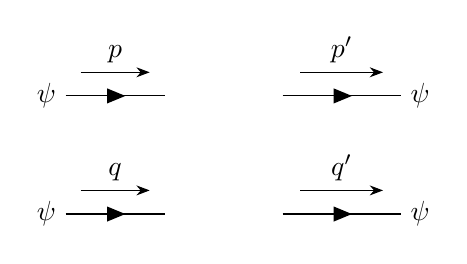
\begin{tikzpicture}
      \begin{feynman}
        \vertex (i1) {$\psi$};
        \vertex [below=of i1] (i2) {$\psi$};
        \vertex [right=of i1] (l1);
        \vertex [right=of l1] (r1);
        \vertex [right=of r1] (f1) {$\psi$};

        \vertex [right=of i2] (l2);
        \vertex [right=of l2] (r2);
        \vertex [right=of r2] (f2) {$\psi$};


        \diagram*{
          (i1) -- [fermion, momentum=$p$] (l1),
          (i2) -- [fermion, momentum=$q$] (l2),

          (r1) -- [fermion, momentum=$p'$] (f1),
          (r2) -- [fermion, momentum=$q'$] (f2),
        };
      \end{feynman}
    \end{tikzpicture}
  \end{center}
  We have initial and final states
  \begin{align*}
    \bket{i} &= \sqrt{4 E_\mathbf{p} E_\mathbf{q}} b_\mathbf{p}^{s\dagger}b_\mathbf{q}^{r\dagger} \bket{0}\\
    \bket{f} &= \sqrt{4 E_{\mathbf{p}'} E_{\mathbf{q}'}} b_{\mathbf{p}'}^{s'\dagger}b_{\mathbf{q}'}^{r'\dagger} \bket{0}.
  \end{align*}
  Here we have to be careful about ordering the creation operators, because they anti-commute, not commute. We then have
  \[
    \brak{f} = \sqrt{4 E_{\mathbf{p}'} E_{\mathbf{q}}} \brak{0} b_{\mathbf{q}'}^{r'} b_{\mathbf{p}'}^{s'}.
  \]
  We can then look at the $O(\lambda^2)$ term in $\brak{f}(S - \mathbf{1})\bket{i}$. We have
  \[
    \frac{(-i\lambda)^2}{2} \int \d^4 x_1 \;\d^4 x_2\; T\Big(\bar\psi(x_1) \psi(x_1) \phi(x_1) \bar\psi(x_2) \psi(x_2) \phi(x_2)\Big)
  \]
  The contribution to scattering comes from the contraction
  \[
    \normalorder{\bar\psi(x_1) \psi(x_1) \bar\psi(x_2) \psi(x_2)} \contraction{}{\phi}{(x_1)}{\phi}\phi(x_1) \phi(x_2).
  \]
  The two $\psi$'s annihilate the initial state, whereas the two $\bar\psi$ create the final state. This is just like the bosonic case, but we have to be careful with minus signs and spinor indices.

  Putting in $\bket{i}$ and ignoring $c$ operators as they don't contribute, we have
  \begin{align*}
    &\hphantom{=}\normalorder{\bar\psi(x_1)\psi(x_1) \bar\psi(x_2) \psi(x_2)} b_\mathbf{p}^{s\dagger}b_{\mathbf{q}}^{r^\dagger}\bket{0}\\
    &= -\int \frac{\d^3 \mathbf{k}_1\;\d^3 \mathbf{k}_2}{(2\pi)^6 2\sqrt{E_{\mathbf{k}_1}E_{\mathbf{k}_2}}} [\bar\psi (x_1) u_{\mathbf{k}_1}^m] [\bar\psi(x_2) u_{\mathbf{k}_2}^n] e^{-ik_1 \cdot x_1 - i k_2 \cdot x_2} b_{\mathbf{k}_1}^m b_{\mathbf{k}_2}^n b_{\mathbf{p}}^{s^\dagger} b_\mathbf{q}^{r\dagger}\bket{0}\\
    \intertext{where the square brackets show contraction of spinor indices}
    &= -\frac{1}{2\sqrt{E_\mathbf{p} E_\mathbf{q}}} \left([\bar\psi(x_1) u_\mathbf{q}^r] [\bar\psi(x_2) u_\mathbf{p}^s] e^{-iq\cdot x_1 - ip\cdot x_2}\right. \\
    &\hphantom{= -\frac{1}{2\sqrt{E_\mathbf{p} E_\mathbf{q}}} \Big(}\left.- [\bar\psi(x_1) u_\mathbf{p}^s][\bar\psi(x_2) u_\mathbf{q}^r] e^{-ip\cdot x - iq\cdot x_2}\right)\bket{0}.
  \end{align*}
  The negative sign, which arose from anti-commuting the $b$'s, is crucial. We put in the left hand side to get
  \begin{align*}
    &\hphantom{=}\brak{0}b_{\mathbf{q}'}^{r'} b_{\mathbf{p}'}^{s'} [\bar\psi(x_1) u_\mathbf{q}^r][\bar\psi(x_2) u_\mathbf{p}^s]\\
    &= \frac{1}{2\sqrt{E_{\mathbf{p}'} E_{\mathbf{q}'}}} \left([\bar u_{\mathbf{p}'}^s u_\mathbf{q}^r][\bar u_{\mathbf{q}'}^{r'} u_\mathbf{p}^s] e^{ip'\cdot x_1 + i q'\cdot x_2} -[\bar{u}_{\mathbf{q}'}^{r'} u_\mathbf{q}^\mathbf{r}][\bar u_{\mathbf{p}'}^{s'} u_{\mathbf{p}}^s] e^{ip'\cdot x_2 + i q'\cdot x_1}\right).
  \end{align*}
  Putting all of this together, including the initial relativistic normalization of the initial state and the propagator, we have
  \begin{align*}
    &\hphantom{=}\brak{f}S - \mathbf{1}\bket{i} \\
    &= (-i\lambda)^2 \int \frac{\d^4 x_1 \; \d^4 x_2}{(2\pi)^4} \frac{\d^3 \mathbf{k}}{(2\pi)^4} \frac{ie^{ik\cdot (x_1 - x_2)}}{k^2 - \mu^2 + i \varepsilon}\\
    &\quad\left([\bar u_{\mathbf{p}'}^{s'} \cdot u_{\mathbf{p}}^s][\bar u_{\mathbf{q}'}^{t'} \cdot u_\mathbf{q}^r] e^{i x_1 \cdot (q' - q) + i x_2 \cdot (p' - p)} - [\bar{u}_{\mathbf{p}'}^{s'}u_\mathbf{q}^r][u_{\mathbf{q}'}^{r'} u_\mathbf{p}^s] e^{ix_1 \cdot (p' - q) + i x_2 \cdot (q' - p)}\right)\\
    &= i(-i\lambda)^2 \int \frac{\d^4 k (2\pi)^4}{k^2 - \mu^2 + i \varepsilon}\left([\bar u_{\mathbf{p}'}^{s'} \cdot u_\mathbf{p}^s][u_{\mathbf{q}'}^{r'} \cdot u_{\mathbf{q}}^r] \delta^4(q' - q + k)\delta^4(p' - p + k)\right.\\
    &\hphantom{= i(-i\lambda)^2 \int \frac{\d^4 k (2\pi)^4}{k^2 - \mu^2 + i \varepsilon}\Big(}\left.- [\bar u_{\mathbf{p}'}^{s'} \cdot u_\mathbf{q}^y][\bar u_{\mathbf{q}'}^{r'} \cdot u_{\mathbf{p}}^s] \delta^4(p' - q + k)\delta^4(q' - p + k)\right).
  \end{align*}
  So we get
  \[
    \brak{f}S - \mathbf{1}\bket{i} = i \mathcal{A}(2\pi)^4 \delta^4(p + q - p' - q'),
  \]
  where
  \[
    \mathcal{A} = (-i \lambda)^2 \left( \frac{[\bar u_{\mathbf{p}'}^{s'} \cdot u_\mathbf{p}^s][\bar u_{\mathbf{q}'}^{r'} \cdot u_\mathbf{q}^r]}{(p' - p)^2 - \mu^2 + i \varepsilon} - \frac{[\bar u_{\mathbf{p}'}^{s'} \cdot u_\mathbf{q}^r][\bar u_{\mathbf{q}'}^{r'} \cdot u_\mathbf{p}^s]}{(q' - p)^2 - \mu^2 + i \varepsilon}\right).
  \]
\end{eg}
\subsection{Feynman rules}
As always, the Feynman rules are much better:
\begin{enumerate}
  \item An incoming fermion is given a spinor $u_\mathbf{p}^r$, and an outgoing fermion is given a $\bar{u}_\mathbf{p}^r$.
    \begin{center}
      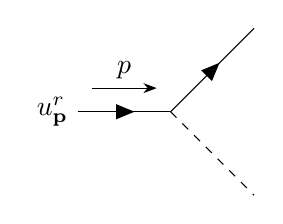
\begin{tikzpicture}
        \begin{feynman}
          \vertex (l) {$u_\mathbf{p}^r$};
          \vertex [right=of l] (m);
          \vertex [above right=of m] (f1);
          \vertex [below right=of m] (f2);
          \diagram*{
            (l) -- [fermion, momentum=$p$] (m) -- [fermion] (f1),
            (m) -- [scalar] (f2),
          };
        \end{feynman}
      \end{tikzpicture}
    \quad\quad
      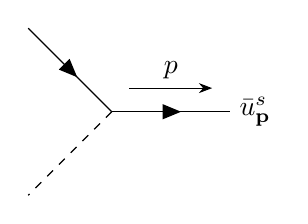
\begin{tikzpicture}
        \begin{feynman}
          \vertex (m);
          \vertex [above left=of m] (i1);
          \vertex [below left=of m] (i2);
          \vertex [right=of m] (f) {$\bar{u}_\mathbf{p}^s$};
          \diagram*{
            (i1) -- [fermion] (m) -- [fermion, momentum=$p$] (f),
            (m) -- [scalar] (i2),
          };
        \end{feynman}
      \end{tikzpicture}
    \end{center}
  \item For an incoming \emph{anti}-fermion, we put in a $\bar{v}_\mathbf{p}^r$, and for an outgoing anti-fermion we put a $v_\mathbf{p}^r$.
    \begin{center}
      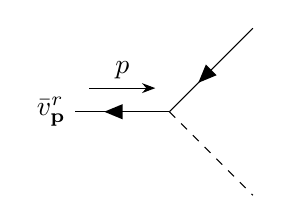
\begin{tikzpicture}
        \begin{feynman}
          \vertex (l) {$\bar v_\mathbf{p}^r$};
          \vertex [right=of l] (m);
          \vertex [above right=of m] (f1);
          \vertex [below right=of m] (f2);
          \diagram*{
            (l) -- [anti fermion, momentum=$p$] (m) -- [anti fermion] (f1),
            (m) -- [scalar] (f2),
          };
        \end{feynman}
      \end{tikzpicture}
    \quad\quad
      \begin{tikzpicture}
        \begin{feynman}
          \vertex (m);
          \vertex [above left=of m] (i1);
          \vertex [below left=of m] (i2);
          \vertex [right=of m] (f) {$v_\mathbf{p}^r$};
          \diagram*{
            (i1) -- [anti fermion] (m) -- [anti fermion, momentum=$p$] (f),
            (m) -- [scalar] (i2),
          };
        \end{feynman}
      \end{tikzpicture}
    \end{center}
  \item For each vertex we get a factor of $(-i\lambda)$.

  \item Each internal scalar line gets a factor of
    \[
      \frac{i}{p^2 - \mu^2 + i \varepsilon},
    \]
    and each internal fermion we get
    \[
      \frac{i(\slashed p + m)}{p^2 - m^2 + i \varepsilon}.
    \]
  \item The arrows on fermion lines must flow consistently, ensuring fermion conservation.
  \item We impose energy-momentum conservation at each vertex, and if we have a loop, we integrate over all possible momentum.
  \item We add an extra minus sign for a loop of fermions.
\end{enumerate}
Note that the Feynman propagator is a $4 \times 4$ matrix. The indices are contracted with each vertex, either with further propagators or external spinors.

We look at computations using Feynman rules.
\begin{eg}[Nucleon scattering]
  For nucleon scattering, we have diagrams
  \begin{center}
    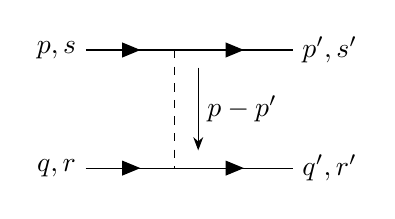
\begin{tikzpicture}
      \begin{feynman}
        \vertex (i1) {$p, s$};
        \vertex [below=of i1] (i2) {$q, r$};
        \vertex [right=of i1] (m1);
        \vertex [right=of i2] (m2);
        \vertex [right=of m1] (f1) {$p', s'$};
        \vertex [right=of m2] (f2) {$q', r'$};

        \diagram*{
          (i1) -- [fermion] (m1) -- [fermion] (f1),
          (i2) -- [fermion] (m2) -- [fermion] (f2),
          (m1) -- [scalar, momentum=$p - p'$] (m2),
        };
      \end{feynman}
    \end{tikzpicture}
    \quad\quad
    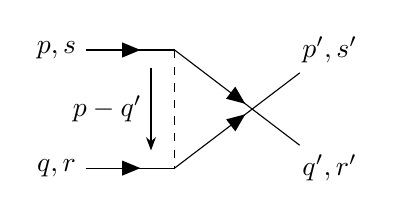
\begin{tikzpicture}
      \begin{feynman}
        \vertex (i1) {$p, s$};
        \vertex [below=of i1] (i2) {$q, r$};
        \vertex [right=of i1] (m1);
        \vertex [right=of i2] (m2);
        \vertex [right=of m1] (f1) {$p', s'$};
        \vertex [right=of m2] (f2) {$q', r'$};

        \diagram*{
          (i1) -- [fermion] (m1) -- [fermion] (f2),
          (i2) -- [fermion] (m2) -- [fermion] (f1),
          (m1) -- [scalar, momentum'=$p - q'$] (m2),
        };
      \end{feynman}
    \end{tikzpicture}
  \end{center}
  In the second case, the fermions are swapped, so we get a relative minus sign. So by the Feynman rules, this contributes an amplitude of
  \[
    \mathcal{A} = (-i \lambda)^2 \left( \frac{[\bar u_{\mathbf{p}'}^{s'} \cdot u_\mathbf{p}^s][\bar u_{\mathbf{q}'}^{r'} \cdot u_\mathbf{q}^r]}{(p' - p)^2 - \mu^2 + i \varepsilon} - \frac{[\bar u_{\mathbf{p}'}^{s'} \cdot u_\mathbf{q}^r][\bar u_{\mathbf{q}'}^{r'} \cdot u_\mathbf{p}^s]}{(q' - p)^2 - \mu^2 + i \varepsilon}\right).
  \]
\end{eg}

\begin{eg}
  We look at nucleon to meson scattering
  \[
    \psi\bar\psi \to \phi \phi.
  \]
  We have two diagrams
  \begin{center}
    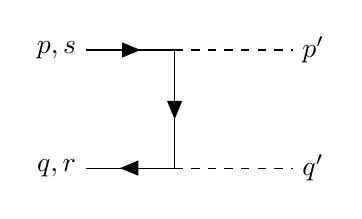
\begin{tikzpicture}
      \begin{feynman}
        \vertex (i1) {$p, s$};
        \vertex [below=of i1] (i2) {$q, r$};
        \vertex [right=of i1] (m1);
        \vertex [right=of i2] (m2);
        \vertex [right=of m1] (f1) {$p'$};
        \vertex [right=of m2] (f2) {$q'$};

        \diagram*{
          (i1) -- [fermion] (m1) -- [fermion] (m2) -- [fermion] (i2),
          (m1) -- [scalar] (f1),
          (m2) -- [scalar] (f2)
        };
      \end{feynman}
    \end{tikzpicture}
    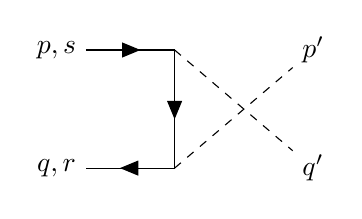
\begin{tikzpicture}
      \begin{feynman}
        \vertex (i1) {$p, s$};
        \vertex [below=of i1] (i2) {$q, r$};
        \vertex [right=of i1] (m1);
        \vertex [right=of i2] (m2);
        \vertex [right=of m1] (f1) {$p'$};
        \vertex [right=of m2] (f2) {$q'$};

        \diagram*{
          (i1) -- [fermion] (m1) -- [fermion] (m2) -- [fermion] (i2),
          (m1) -- [scalar] (f2),
          (m2) -- [scalar] (f1)
        };
      \end{feynman}
    \end{tikzpicture}
  \end{center}
  This time, we flipped two bosons, so we are not gaining a negative sign. Then the Feynman rules give us
  \[
    \mathcal{A} = (-i\lambda)^2 \left(\frac{\bar{v}_\mathbf{q}^r (\slashed p - \slashed p' + m) u_\mathbf{p}^s}{(p - p')^2 - m^2 + i \varepsilon} + \frac{\bar v_\mathbf{q}^r (\slashed p - \slashed q' + m) u_\mathbf{p}^s}{(p - q')^2 - m^2 + i \varepsilon}\right).
  \]
\end{eg}

\begin{eg}
  We can also do nucleon anti-nucleon scattering
  \[
    \psi\bar\psi \to \psi\bar\psi.
  \]
  As before, we have two contributions
  \begin{center}
    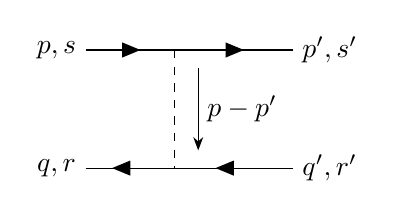
\begin{tikzpicture}
      \begin{feynman}
        \vertex (i1) {$p, s$};
        \vertex [below=of i1] (i2) {$q, r$};
        \vertex [right=of i1] (m1);
        \vertex [right=of i2] (m2);
        \vertex [right=of m1] (f1) {$p', s'$};
        \vertex [right=of m2] (f2) {$q', r'$};

        \diagram*{
          (i1) -- [fermion] (m1) -- [fermion] (f1),
          (i2) -- [anti fermion] (m2) -- [anti fermion] (f2),
          (m1) -- [scalar, momentum=$p - p'$] (m2),
        };
      \end{feynman}
    \end{tikzpicture}

    \begin{tikzpicture}
      \begin{feynman}
        \vertex (m1);
        \vertex [above left=of m1] (i1) {$p, s$};
        \vertex [below left=of m1] (i2) {$q, r$};
        \vertex [right=of m1] (m2);
        \vertex [above right=of m2] (f1) {$p', s'$};
        \vertex [below right=of m2] (f2) {$q', r'$};

        \diagram*{
          (i1) -- [fermion] (m1) -- [fermion] (i2),
          (f2) -- [fermion] (m2) -- [fermion] (f1),
          (m1) -- [scalar] (m2),
        };
      \end{feynman}
    \end{tikzpicture}
  \end{center}
  This time we have an amplitude of
  \[
    \mathcal{A} = (-i\lambda)^2 \left(\frac{-[\bar u_{\mathbf{p}'}^{s'} \cdot u_\mathbf{p}^s][\bar v_\mathbf{q}^r \cdot v_{\mathbf{q}'}^{r'}]}{(p - p')^2 - \mu^2 + i \varepsilon} + \frac{[\bar{v_\mathbf{q}}^r \cdot u_\mathbf{p}^s][\bar u_{\mathbf{p}'}^{s'} \cdot v_{\mathbf{q}'}^{r'}]}{(p + q)^2 - \mu^2 + i \varepsilon}\right).
  \]
  We have these funny signs that we have to make sure are right. We have an initial state
  \begin{align*}
    \bket{i} &= \sqrt{4 E_\mathbf{p} E_\mathbf{q}} b_\mathbf{p}^{s\dagger}c_\mathbf{q}^{r\dagger}\bket{0} \equiv \bket{\mathbf{p}, s; \mathbf{q}, r}\\
    \bket{f} &= \sqrt{4E_{\mathbf{p}'} E_{\mathbf{q}'}} b_{\mathbf{p}'} ^{s'\dagger} c_{\mathbf{q}'}^{r'\dagger} \bket{0} \equiv \bket{\mathbf{p}', s'; \mathbf{q}', r'}
  \end{align*}
  To check the signs, we work through the computations, but we can ignore all factors because we only need the final sign. Then we have
  \begin{align*}
    \psi &\sim b + c^\dagger\\
    \bar\psi &\sim b^\dagger + c
  \end{align*}
  So we can check
  \begin{align*}
    &\hphantom{=} \brak{f} \normalorder{\bar\psi(x_1) \psi(x_1) \bar\psi(x_2) \psi(x_2)} b_\mathbf{p}^{s\dagger} c_{\mathbf{q}}^{r\dagger}\bket{0}\\
    &\sim \brak{f} [\bar{v}_{\mathbf{k}_1}^m \psi(x_1)][\bar\psi(x_2) u_{\mathbf{k}_2}^n] c_{\mathbf{k}_1}^m b_{\mathbf{k}_2}^n b_{\mathbf{p}}^{s\dagger} c_{\mathbf{q}}^{r\dagger}\bket{0}\\
    &\sim \brak{f}[\bar{v}_{\mathbf{q}}^m \psi(x_1)][\bar\psi(x_2) u_{\mathbf{p}}^n]\bket{0}\\
    &\sim \brak{0}c_{\mathbf{q}'}^{r'} b_{\mathbf{p}'}^{s'} c_{\boldsymbol\ell_1}^{m\dagger} b_{\boldsymbol\ell_2}^{n^\dagger} [\bar{v}_{\mathbf{q}}^r \cdot v_{\boldsymbol{\ell}_1}^m][\bar{u}_{\boldsymbol{\ell}_2}^n \cdot u_\mathbf{p}^s ]\bket{0}\\
    &\sim -[\bar{v}_\mathbf{q}^r \cdot v_{\mathbf{q}'}^{r'}][\bar{u}_{\mathbf{p}'}^{s'} \cdot u_\mathbf{p}^s],
  \end{align*}
  where we got the final sign by anti-commuting $c_{\mathbf{\ell}_1}^{m\dagger}$ and $b_{\mathbf{p}'}^{s'}$ to make the $c$'s and $b$'s get together.

  We can follow a similar contraction to get a positive sign for the second diagram.
\end{eg}

\section{Quantum electrodynamics}
Finally, we get to the last part of the course, where we try to quantize electromagnetism. Again, this will not be so straightforward. This time, we will have to face the fact that the electromagnetic potential $A$ is not uniquely defined, but can have many gauge transformations. The right way to encode this information when we quantize the theory is not immediate, and will require some experimentation.

\subsection{Classical electrodynamics}
We begin by reviewing what we know about classical electrodynamics. Classically, the electromagnetic field is specified by an \term{electromagnetic potential} $A$, from which we derive the \term{electromagnetic field strength tensor}
\[
  F_{\mu\nu} = \partial_\mu A_\nu - \partial_\nu A_\mu,
\]
We can then find the dynamics of a free electromagnetic field by
\[
  \mathcal{L} = -\frac{1}{4} F_{\mu\nu}F^{\mu\nu}.
\]
The Euler-Lagrange equations give
\[
  \partial_\mu F^{\mu\nu} = 0.
\]
It happens that $F$ satisfies the mystical \term{Bianchi identity}
\[
  \partial_\lambda F_{\mu\nu} + \partial_\mu F_{\nu\lambda} + \partial_\nu F_{\lambda\mu} = 0,
\]
but we are not going to use this.

We can express these things in terms of the electromagnetic field. We write $A = (\phi, \mathbf{A})$. Then we define
\[
  \mathbf{E} = - \nabla \phi - \dot{\mathbf{A}},\quad \mathbf{B} = \nabla\wedge \mathbf{A}.
\]
Then $F_{\mu\nu}$ can be written as
\[
  F_{\mu\nu} =
  \begin{pmatrix}
    0 & E_x & E_y & E_z\\
    -E_x & 0 & -B_z & B_y\\
    -E_y & B_z & 0 & -B_x\\
    -E_z & -B_y & B_x & 0
  \end{pmatrix}
\]
Writing out our previous equations, we find that
\begin{align*}
  \nabla \cdot \mathbf{E} &= 0\\
  \nabla \cdot \mathbf{B} &= 0\\
  \dot{\mathbf{B}} &= - \nabla \wedge \mathbf{E}\\
  \dot{\mathbf{E}} &= \nabla \wedge \mathbf{B}.
\end{align*}
We notice something wrong. Photons are excitations of the electromagnetic field. However, the photon only has two polarization states, i.e.\ two degrees of freedom, while this vector field $A^\mu$ has four. How can we resolve this?

There are two parts to the resolution. Firstly, note that the $A_0$ field is not dynamical, as it has no kinetic term in the Lagrangian (the $\partial_0 A_0$ terms cancel out by symmetry). Thus, if we're given $A_i$ and $\dot{A}_i$ at some initial time $t_0$, then $A_0$ is fully determined by $\nabla \cdot \mathbf{E} = 0$, since it says
\[
  \nabla \cdot \dot{\mathbf{A}} + \nabla^2 A_0 = 0.
\]
This has a solution
\[
  A_0(\mathbf{x}) = \int \d^3 \mathbf{x} \frac{\nabla \cdot \dot{\mathbf{A}}(\mathbf{x}')}{4\pi(\mathbf{x} - \mathbf{x}')}.
\]
So $A_0$ is \emph{not} independent, and we've got down to three degrees of freedom. What's the remaining one?

The next thing to note is that the theory is invariant under the transformation
\[
  A_\mu (x) \mapsto A_\mu(x) + \partial_\mu \lambda(x),
\]
Indeed, the only ``observable'' thing is $F_{\mu\nu}$, and we can see that it transforms as
\[
  F_{\mu\nu} \mapsto \partial_\mu (A_\nu + \partial_\nu \lambda) - \partial_\nu(A_\mu + \partial_\mu \lambda) = F_{\mu\nu}.
\]
It looks like that we now have an infinite number of symmetries.

This is a different kind of symmetry. Previously, we had symmetries acting at all points in the universe in the same way, say $\psi \mapsto e^{i\alpha}\psi$ for some $\alpha \in \R$. This gave rise to conservation laws by Noether's theorem.

Now do we get infinitely many symmetries from Noether's theorem? The answer is no. The local symmetries we're considering now have a different interpretation. Rather than taking a physical state to another physical state, they are really a redundancy in our description. These are known as \emph{local} or \term{gauge symmetries}\index{local symmetries}.
%
%One way to see this redundancy is to notice that Maxwell's equations do not specify the evolutions of $A_\mu$. The equations read
%\[
% (\eta_{\mu\nu} \partial_\rho \partial^\rho - \partial_\mu \partial_\nu) A^\nu = 0.
%\]
%The differential operator is not invertible, and in fact annihilates any function of the form $\partial_\mu \lambda(x)$.
%
%This means that given $A_i$ and $\dot{A}_i$ at $t_0$, we have no way to uniquely determine the evolution of $A_\mu$. So we can't distinguish between $A_\mu$ and $A_\mu + \partial_\mu \lambda(x)$.
%
%This might seem problematic, but it is fine as long as $A_\mu$ and $A_\mu + \partial_\mu \lambda(x)l$ correspond to the same physical state.
%
Seeing this, we might be tempted to try to formulate the theory only in terms of gauge invariant objects like $\mathbf{E}$ and $\mathbf{B}$, but it turns out this doesn't work. To describe nature, it appears that we have to introduce quantities that we cannot measure.

Now to work with our theory, it is common to \emph{fix a gauge}. The idea is that we specify some additional rules we want $A_\mu$ to satisfy, and hopefully this will make sure there is a unique $A_\mu$ we can pick for each equivalence class. Picking the right gauge for the right problem can help us a lot. This is somewhat like picking a coordinate system. For example, in a system with spherical symmetry, using spherical polar coordinates will help us a lot.

There are two gauges we would be interested in.
\begin{defi}[Lorenz gauge]\index{Lorenz gauge}
  The \emph{Lorenz gauge} is specified by
  \[
    \partial_\mu A^\mu = 0
  \]
\end{defi}
Note that this is Lorenz, \emph{not} Lorentz!

To make sure this is a valid gauge, we need to make sure that each electromagnetic potential has a representation satisfying this condition.

Suppose we start with $A_\mu'$ such that $\partial_\mu A'^\mu = f$. If we introduce a gauge transformation
\[
  A_\mu = A_\mu' + \partial_\mu \lambda,
\]
then we have
\[
  \partial_\mu A^\mu = \partial_\mu \partial^\mu \lambda + f.
\]
So we need to find a $\lambda$ such that
\[
  \partial_\mu \partial^\mu \lambda = -f.
\]
By general PDE theory, such a $\lambda$ exists. So we are safe.

However, it turns out this requirement does not pick a unique representation in the gauge orbit. We are free to make a further gauge transformation by with
\[
  \partial_\mu \partial^\mu \lambda = 0,
\]
which has non-trivial solutions (e.g.\ $\lambda(x) = x^0$).

Another important gauge is the Coulomb gauge:
\begin{defi}[Coulomb gauge]\index{Coulomb gauge}
  The \emph{Coulomb gauge} requires
  \[
    \nabla \cdot \mathbf{A} = 0.
  \]
\end{defi}
Of course, this is not a Lorentz-invariant condition.

Similar to the previous computations, we know that this is a good gauge. Looking at the integral we've found for $A_0$ previously, namely
\[
  A_0 = \int \d^3 \mathbf{x}' \frac{\nabla \cdot \dot{\mathbf{A}}(\mathbf{x}')}{4\pi|\mathbf{x} - \mathbf{x}'|},
\]
we find that $A_0 = 0$ all the time. Note that this happens only because we do not have matter.

Here it is easy to see the physical degrees of freedom --- the three components in $\mathbf{A}$ satisfy a single constraint $\nabla \cdot \mathbf{A} = 0$, leaving behind two physical degrees of freedom, which gives the desired two polarization states.

\subsection{Quantization of the electromagnetic field}
We now try to quantize the field, using the Lorenz gauge. The particles we create in this theory would be photons, namely quanta of light. Things will go wrong really soon.

We first try to compute the conjugate momentum $\pi^\mu$ of the vector field $A^\mu$. We have
\[
  \pi^0 = \frac{\partial \mathcal{L}}{\partial \dot{A}_0} = 0.
\]
This is slightly worrying, because we would later want to impose the commutation relation
\[
  [A_0(\mathbf{x}), \pi^0(\mathbf{y})] = i \delta^3(\mathbf{x} - \mathbf{y}),
\]
but this is clearly not possible if $\pi^0$ vanishes identically!

We need to try something else. Note that under the Lorenz gauge $\partial_\mu A^\mu = 0$, the equations of motion tell us
\[
  \partial_\mu \partial^\mu A^\nu = 0.
\]
The trick is to construct a Lagrangian where this is actually the equation of motion, and then later impose $\partial_\mu A^\mu = 0$ after quantization.

This is not too hard. We can pick the Lagrangian as
\[
  \mathcal{L} = -\frac{1}{4} F_{\mu\nu}F^{\mu\nu} - \frac{1}{2}(\partial_\mu A^\mu)^2.
\]
We can work out the equations of motion of this, and we get
\[
  \partial_\mu F^{\mu\nu} + \partial^\nu(\partial_\mu A^\mu) = 0.
\]
Writing out the definition of $F^{\mu\nu}$, one of the terms cancels with the second bit, and we get
\[
  \partial_\mu \partial^\mu A^\nu = 0.
\]
We are now going to work with this Lagrangian, and only later impose $\partial_\mu A^\mu = 0$ at the operator level.

More generally, we can use a Lagrangian
\[
  \mathcal{L} =- \frac{1}{4}F_{\mu\nu}F^{\mu\nu} - \frac{1}{2\alpha} (\partial_\mu A^\mu)^2,
\]
where $\alpha$ is a fixed constant. Confusingly, the choice of $\alpha$ is also known as a gauge. We picked $\alpha = 1$, which is called the \term{Feynman gauge}. If we take $\alpha \to 0$, we obtain the \term{Landau gauge}.

This new theory has no gauge symmetry, and both $A_0$ and $\mathbf{A}$ are dynamical fields. We can find the conjugate momenta as
\begin{align*}
  \pi^0 &= \frac{\partial\mathcal{L}}{\partial \dot{A}_0} = - \partial_\mu A^\mu\\
  \pi^i &= \frac{\partial \mathcal{L}}{\partial \dot{A}_i} = \partial^i A^0 - \dot{A}^i.
\end{align*}
We now apply the usual commutation relations
\begin{gather*}
  [A_\mu (\mathbf{x}), A_\nu(\mathbf{y})] = [\pi^\mu(\mathbf{x}), \pi^\nu(\mathbf{y})] = 0\\
  [A_\mu(\mathbf{x}), \pi^\nu(\mathbf{y})] = i\delta^3(\mathbf{x} - \mathbf{y}) \delta_\mu^\nu.
\end{gather*}
Equivalently, the last commutation relation is
\[
  [A_\mu(\mathbf{x}), \pi_\nu(\mathbf{y})] = i\delta^3(\mathbf{x} - \mathbf{y}) \eta_{\mu\nu}.
\]
As before, in the Heisenberg picture, we get equal time commutation relations
\[
  [A_\mu (\mathbf{x}, t), \dot{A}_\nu(\mathbf{y}, t)] = i\eta_{\mu\nu} \delta^3(\mathbf{x} - \mathbf{y}).
\]
As before, we can write our operators in terms of creation and annihilation operators:
\begin{align*}
  A_\mu(\mathbf{x}) &= \int \frac{\d^3 \mathbf{p}}{(2\pi)^3} \frac{1}{\sqrt{2 |\mathbf{p}|}} \sum_{\lambda = 0}^3 \mathcal{E}_\mu^{(\lambda)}(\mathbf{p}) [a_\mathbf{p}^\lambda e^{i\mathbf{p}\cdot \mathbf{x}} + a_\mathbf{p}^{\lambda\dagger} e^{-i\mathbf{p}\cdot \mathbf{x}}],\\
  \pi^\nu(\mathbf{x}) &= \int \frac{\d^3 \mathbf{p}}{(2\pi)^3} i\sqrt{\frac{|\mathbf{p}|}{2}} \sum_{\lambda = 0}^3 (\mathcal{E}^{(\lambda)}(\mathbf{p}))^\nu [a_\mathbf{p}^\lambda e^{i\mathbf{p}\cdot \mathbf{x}} - a_\mathbf{p}^{\lambda\dagger} e^{-i\mathbf{p}\cdot \mathbf{x}}],
\end{align*}
where for each $\mathbf{p}$, the vectors $\{\mathcal{E}^{(0)}(\mathbf{p}), \mathcal{E}^{(1)}(\mathbf{p}), \mathcal{E}^{(2)}(\mathbf{p}), \mathcal{E}^{(3)}(\mathbf{p})\}$ form a basis of $\R^{3, 1}$. The exact choice doesn't really matter much, but we will suppose we pick a basis with the following properties:
\begin{enumerate}
  \item $\mathcal{E}^{(0)}(\mathbf{p})$ will be a timelike vector, while the others are spacelike.
  \item Viewing $\mathbf{p}$ as the direction of motion, we will pick $\mathcal{E}^{(3)}(\mathbf{p})$ to be a longitudinal polarization, while $\mathcal{E}^{(1),(2)}(\mathbf{p})$ are transverse to the direction of motion, i.e.\ we require
    \[
      \mathcal{E}^{(1), (2)}_\mu(\mathbf{p}) \cdot p^\mu = 0.
    \]
  \item The normalization of the vectors is given by
    \[
      \mathcal{E}^{(\lambda)}_\mu (\mathcal{E}^{(\lambda')})^\mu = \eta^{\lambda\lambda'},
    \]
\end{enumerate}

We can explicitly write down a choice of such basis vectors. When $p \propto (1, 0, 0, 1)$, then we choose
\[
  \mathcal{E}^{(0)}_\mu(\mathbf{p}) =
  \begin{pmatrix}
    1\\0\\0\\0
  \end{pmatrix},\quad
  \mathcal{E}^{(1)}_\mu(\mathbf{p}) =
  \begin{pmatrix}
    0\\1\\0\\0
  \end{pmatrix},\quad
  \mathcal{E}^{(2)}_\mu(\mathbf{p}) =
  \begin{pmatrix}
    0\\0\\1\\0
  \end{pmatrix},\quad
  \mathcal{E}^{(3)}_\mu(\mathbf{p}) =
  \begin{pmatrix}
    0\\0\\0\\1
  \end{pmatrix}.
\]
Now for a general $p$, we pick a basis where $p \propto (1, 0, 0, 1)$, which is always possible, and then we define $\mathcal{E}(\mathbf{p})$ as above in that basis. This gives us a Lorentz-invariant choice of basis vectors satisfying the desired properties.

One can do the tedious computations required to find the commutation relations for the creation and annihilation operators:
\begin{thm}
  \[
    [a_\mathbf{p}^\lambda, a_\mathbf{q}^{\lambda'}] = [a_\mathbf{p}^{\lambda\dagger}, a_\mathbf{q}^{\lambda'\dagger}] = 0
  \]
  and
  \[
    [a_\mathbf{p}^\lambda, a_\mathbf{q}^{\lambda' \dagger}] = -\eta^{\lambda\lambda'} (2\pi)^3 \delta^3(\mathbf{p} - \mathbf{q}).
  \]
\end{thm}
Notice the strange negative sign!

We again define a vacuum $\bket{0}$ such that
\[
  a_\mathbf{p}^\lambda \bket{0} = 0
\]
for $\lambda = 0, 1, 2, 3$, and we can create one-particle states
\[
  \bket{\mathbf{p}, \lambda} = a_\mathbf{p}^{\lambda\dagger} \bket{0}.
\]
This makes sense for $\lambda = 1, 2, 3$, but for $\lambda = 0$, we have states with negative norm:
\begin{align*}
  \braket{\mathbf{p}, 0}{\mathbf{q}, 0} &\equiv \brak{0} a_\mathbf{p}^0 a_\mathbf{q}^{0\dagger}\bket{0}\\
  &= -(2\pi)^3 \delta^3(\mathbf{p} - \mathbf{q}).
\end{align*}
A Hilbert space with a negative norm means that we have negative probabilities. This doesn't make sense.

Here is where the Lorenz gauge comes in. By imposing $\partial_\mu A^\mu = 0$, we are going to get rid of bad things. But how do we implement this constraint? We can try implementing it in a number of ways. We will start off in the obvious way, which turns out to be too strong, and we will keep on weakening it until it works.

If we just asked for $\partial_\mu A^\mu = 0$, for $A^\mu$ the operator, then this doesn't work, because
\[
  \pi^0 = - \partial_\mu A^\mu,
\]
and if this vanishes, then the commutation conditions cannot possibly be obeyed.

Instead, we can try to impose this on the Hilbert space rather than on the operators. After all, that's where the trouble lies. Maybe we can try to split the Hilbert space up into good states and bad states, and then just look at the good states only?

How do we define the good, physical states? Maybe we can impose
\[
  \partial_\mu A^\mu \bket{\psi} = 0
\]
on all physical (``good'') states, but it turns out even this condition is a bit too strong, as the vacuum will not be physical! To see this, we decompose
\[
  A_\mu(x) = A_\mu^+ (x) + A_\mu^-(x),
\]
where $A_\mu^+$ has the annihilation operators and $A_\mu^-$ has the creation operators. Explicitly, we have
\begin{align*}
  A_\mu^+(x) &= \int \frac{\d^3 \mathbf{p}}{(2\pi)^3} \frac{1}{\sqrt{2|\mathbf{p}|}} \mathcal{E}_\mu^{(\lambda)} a_\mathbf{p}^\lambda e^{-i p\cdot x}\\
  A_\mu^-(x) &= \int \frac{\d^3 \mathbf{p}}{(2\pi)^3} \frac{1}{\sqrt{2|\mathbf{p}|}} \mathcal{E}_\mu^{(\lambda)} a_\mathbf{p}^{\lambda\dagger} e^{ip\cdot x},
\end{align*}
where summation over $\lambda$ is implicit. Then we have
\[
  \partial^\mu A_\mu^+\bket{0} = 0,
\]
but we have
\[
  \partial^\mu A_\mu^- \bket{0} \not= 0.
\]
So not even the vacuum is physical! This is very bad.

Our final attempt at weakening this is to ask the physical states to satisfy
\[
  \partial^\mu A_\mu^+(x) \bket{\psi} = 0.
\]
This ensures that
\[
  \brak{\psi}\partial^\mu A_\mu \bket{\psi} = 0,
\]
as $\partial^\mu A_\mu^+$ will kill the right hand side and $\partial^\mu A_\mu^-$ will kill the left. So $\partial_\mu A^\mu$ has vanishing matrix elements between physical states.

This is known as the \term{Gupta-Bleuler condition}. The linearity of this condition ensures that the physical states span a vector space $\mathcal{H}_{\mathrm{phys}}$.

What does $\mathcal{H}_{\mathrm{phys}}$ look like? To understand this better, we write out what $\partial^\mu A_\mu^-$ is. We have
\begin{align*}
  \partial^\mu A_\mu^- &= \int \frac{\d^3 \mathbf{p}}{(2\pi)^3} \frac{1}{\sqrt{2|\mathbf{p}|}} \mathcal{E}_\mu^{(\lambda)} a_\mathbf{p}^{\lambda} (-ip^\mu) e^{-ip\cdot x}\\
  &= \int \frac{\d^3 \mathbf{p}}{(2\pi)^3} \frac{1}{\sqrt{2|\mathbf{p}|}} i(a_\mathbf{p}^3 - a_\mathbf{p}^0) e^{ip\cdot x},
\end{align*}
using the properties of our particular choice of the $\mathcal{E}^\mu$. Thus the condition is equivalently
\[
  (a_\mathbf{p}^3 - a_\mathbf{p}^0)\bket{\psi} = 0.
\]
This means that it is okay to have a timelike or longitudinal photons, as long as they come in pairs of the same momentum!

By restricting to these physical states, we have gotten rid of the negative norm states. However, we still have the problem of certain non-zero states having zero norm. Consider a state
\[
  \bket{\phi} = a_\mathbf{p}^{0\dagger} a_\mathbf{p}^{3\dagger}\bket{0}.
\]
This is an allowed state, since it has exactly one timelike and one longitudinal photon, each of momentum $\mathbf{p}$. This has zero norm, as the norm contributions from the $a_\mathbf{p}^0$ part cancel from those from the $a_\mathbf{p}^3$ part. However, this state is non-zero! We wouldn't want this to happen if we want a positive definite inner product.

The solution is to declare that if two states differ only in the longitudinal and timelike photons, then we consider them \emph{physically equivalent}, or gauge equivalent! In other words, we are quotienting the state space out by these zero-norm states.

Of course, if we want to do this, we need to go through everything we do and make sure that our physical observables do not change when we add or remove these silly zero-norm states. Fortunately, this is indeed the case, and we are happy.

%This suggests we should treat the longitudinal/timelike parts and the transverse parts separately. For any basis state $\bket{\psi}$ in the Fock space, we write it as
%\[
% \bket{\psi} = \bket{\psi_T} \bket{\phi},
%\]
%where $\bket{\psi_T}$ contains the transverse photons, and $\bket{\phi}$ contains the timelike or longitudinal ones. Then we can rewrite our condition as
%\[
% (a_\mathbf{p}^3 - a_\mathbf{p}^0) \bket{\phi} = 0.
%\]
%Assuming this condition, we can write
%\[
% \bket{\phi} = \sum_{n = 0}^\infty c_n \bket{\phi_n},
%\]
%where each $\phi_n$ is a sum of $2n$-particle states, with each state containing $n$ timelike and $n$ longitudinally polarized photons of the same momenta. We have $\brak{\phi_0} = \bket{0}$, and by convention, we pick $c_0 = 1$ (we can shift the factors to $\bket{\psi_T}$). These states satisfy
%\[
% \braket{\phi_n}{\phi_m} = \delta_{n0} \delta_{m0}.
%\]
%So in particular, we have
%\[
% \braket{\phi}{\phi} = c_0 \braket{\phi_0}{\phi_0} = c_0 = 1,
%\]
%Thus, we know that
%\[
% \braket{\psi}{\psi} = \braket{\psi_T}{\psi_T}.
%\]
%This means, in particular, that
%and all negative normed states are moved by $(*)$. We treat the zero normed states as being \emph{gauge equivalent} to the vacuum. % are we quotienting out by the subspace?
%
%Two states which differ only in the longitudinal or timelike photons are said to be \term{physically equivalent}. Of course, this makes sense only if no physical observables depend on these $\phi_n$ (for $n > 0$). In particular, we should check that the Hamiltonian indeed doesn't depend on these states, but this is boring, and we will just state the result. We have
%\[
% H = \int \frac{\d^3 \mathbf{p}}{(2\pi)^3} |\mathbf{p}| \left(\sum_{i = 1}^3 a_\mathbf{p}^{i\dagger} a_\mathbf{p}^i - a_\mathbf{p}^{0\dagger}a_\mathbf{p}^0\right).
%\]
%But we require that $a_\mathbf{k}^3 - a_\mathbf{k}^0 \bket{\psi} = 0$. So we have
%\[
% \bra \psi a_\mathbf{p}^{3\dagger}a_\mathbf{p}^3 \bket{\psi} = \bra{\psi}a_\mathbf{p}^{0\dagger}a_\mathbf{p}^0 \bket{\psi}.
%\]
%So time-like and longitudinal pieces cancel in $H$. We just get contributions from the transverse states.
%
%In general, any matrix elements involving any gauge-invariant operator evalluated on physical states are independent of the $c_n$.

Before we move on, we note the value of the Feynman propagator:

\begin{thm}
  The Feynman propagator for the electromagnetic field, under a general gauge $\alpha$, is
  \[
    \brak{0} TA_\mu(x) A_\nu(y) \bket{0} = \int \frac{\d^4 p}{(2\pi)^4} \frac{-i}{p^2 + i\varepsilon} \left(\eta_{\mu\nu} + (\alpha - 1) \frac{p_\mu p_\nu}{p^2}\right) e^{-ip\cdot(x - y)}.
  \]
\end{thm}

\subsection{Coupling to matter in classical field theory}
We now move on to couple our EM field with matter. We first do it in the clear and sensible universe of classical field theory. We will tackle two cases --- in the first case, we do coupling with fermions. In the second, we couple with a mere complex scalar field. It should be clear one how one can generalize these further to other fields.

Suppose the resulting coupled Lagrangian looked like
\[
  \mathcal{L} = - \frac{1}{4} F_{\mu\nu}F^{\mu\nu} - A_\mu j^\mu,
\]
plus some kinetic and self-interaction terms for the field we are coupling with. Then the equations of motion give us
\[
  \partial_\mu F^{\mu\nu} = j^\nu.
\]
Since $F_{\mu\nu}$ is anti-symmetric, we know we must have
\[
  0 = \partial_\mu \partial_\nu F^{\mu\nu} = \partial_\nu j^\nu.
\]
So we know $j^\mu$ is a conserved current. So to couple the EM field to matter, we need to find some conserved current.

\subsubsection*{Coupling with fermions}
Suppose we had a spinor field $\psi$ with Lagrangian
\[
  \mathcal{L} = \bar\psi (i \slashed\partial -m ) \psi.
\]
This has an internal symmetry
\begin{align*}
  \psi &\mapsto e^{-i\alpha \psi}\\
  \bar\psi &\mapsto e^{i \alpha} \bar\psi,
\end{align*}
and this gives rise to a conserved current
\[
  j^\mu = \bar\psi \gamma^\mu \psi.
\]
So let's try
\[
  \mathcal{L} = -\frac{1}{4}F_{\mu\nu}F^{\mu\nu} + \bar\psi(i \slashed \partial- m)\psi - e \bar\psi \gamma^\mu A_\mu \psi,
\]
where $e$ is some coupling factor.

Have we lost gauge invariance now that we have an extra term? If we just substituted $A_\mu$ for $A_\mu + \partial_\mu \lambda$, then obviously the Lagrangian changes. However, something deep happens. When we couple the two terms, we don't just add a factor into the Lagrangian. We have secretly introduced a new gauge symmetry to the fermion field, and now when we take gauge transformations, we have to transform both fields at the same time.

To see this better, we rewrite the Lagrangian as
\[
  \mathcal{L} = -\frac{1}{4} F_{\mu\nu} F^{\mu\nu} + \bar\psi(i \slashed \D - m)\psi,
\]
where $\D$ is the \term{covariant derivative} given by
\[
  \D_\mu \psi = \partial_\mu \psi + i e A_\mu \psi.
\]
We now claim that $\mathcal{L}$ is invariant under the simultaneous transformations
\begin{align*}
  A_\mu &\mapsto A_\mu + \partial_\mu \lambda(x)\\
  \psi &\mapsto e^{-ie \lambda(x)} \psi.
\end{align*}
To check that this is indeed invariant, we only have to check that $\bar\psi\slashed \D \psi$ term. We look at how $\D_\mu \psi$ transforms. We have
\begin{align*}
  \D_\mu \psi &= \partial_\mu \psi + ie A_\mu \psi\\
  &\mapsto \partial_\mu (e^{-ie\lambda(x)} \psi) + ie (A_\mu + \partial_\mu \lambda(x)) e^{-ie\lambda(x)}\psi\\
  &= e^{-ie\lambda(x)} \D_\mu\psi.
\end{align*}
So we have
\[
  \bar\psi \slashed \D \psi \mapsto \bar\psi \slashed \D \psi,
\]
i.e.\ this is gauge invariant.

So as before, we can use the gauge freedom to remove unphysical states after quantization. The coupling constant $e$ has the interpretation of electric charge, as we can see from the equation of motion
\[
  \partial_\mu F^{\mu\nu} = ej^\nu.
\]
In electromagnetism, $j^0$ is the charge density, but after quantization, we have
\begin{align*}
  Q &= e \int \d^3 \mathbf{x}\; \bar\psi \gamma^0 \psi \\
  &= \int \frac{\d^3 \mathbf{p}}{(2\pi)^3} (b_\mathbf{p}^{s\dagger} b_\mathbf{p}^s - c_\mathbf{p}^{s\dagger} c_\mathbf{p}^s)\\
  &= e \times (\text{number of electrons} - \text{number of anti-electrons}),
\end{align*}
with an implicit sum over the spin $s$. So this is the total charge of the electrons, where anti-electrons have the opposite charge!

For QED, we usually write $e$ in terms of the fine structure constant
\[
  \alpha = \frac{e^2}{4\pi} \approx \frac{1}{137}
\]
for an electron.

\subsubsection*{Coupling with complex scalars}
Now let's try to couple with a scalar fields. For a real scalar field, there is no suitable conserved current to couple $A^\mu$ to. For a complex scalar field $\varphi$, we can use the current coming from $\varphi \to e^{i\alpha} \varphi$, namely
\[
  j_\mu = (\partial_\mu \varphi)^* \varphi - \varphi^* \partial_\mu \varphi.
\]
We try the obvious thing with an interaction term
\[
  \mathcal{L}_{\mathrm{int}} = -i [(\partial_\mu \varphi)^* \varphi - \varphi^* \partial_\mu \varphi] A^\mu
\]
This doesn't work. The problem is that we have introduced a new term $j^\mu A_\mu$ to the Lagrangian. If we compute the conserved current due to $\varphi \mapsto e^{i\alpha} \varphi$ under the new Lagrangian, it turns out we will obtain a \emph{different} $j^\mu$, which means in this theory, we are not really coupling to the conserved current, and we find ourselves going in circles.

To solve this problem, we can try random things and eventually come up with the extra term we need to add to the system to make it consistent, and then be perpetually puzzled about why that worked. Alternatively, we can also learn from what we did in the previous example. What we did, at the end, was to invent a new covariant derivative:
\[
  \D_\mu \varphi = \partial_\mu \varphi + ie A_\mu \varphi,
\]
and then replace all occurrences of $\partial_\mu$ with $\D_\mu$. Under a simultaneous gauge transformation
\begin{align*}
  A_\mu &\mapsto A_\mu + \partial_\mu \lambda(x)\\
  \varphi &\mapsto e^{-ie \lambda(x)} \varphi,
\end{align*}
the covariant derivative transforms as
\[
  \D_\mu \varphi \mapsto e^{i\lambda(x)} \D_\mu \varphi,
\]
as before. So we can construct a gauge invariant Lagrangian by
\[
  \mathcal{L} = -\frac{1}{4} F_{\mu\nu}F^{\mu\nu} + (\D_\mu \varphi)^\dagger (\D^\mu \varphi) - m^2 \varphi^* \varphi.
\]
The current is the same thing as we've had before, except we have
\[
  j^\mu = i(\D_\mu \varphi)^\dagger \varphi - \varphi^\dagger \D_\mu \varphi.
\]
In general, for any field $\phi$ taking values in a complex vector space, we have a $\U(1)$ gauge symmetry
\[
  \phi \mapsto e^{i\lambda(x)} \phi.
\]
Then we can couple with the EM field by replacing
\[
  \partial_\mu \phi \mapsto \D_\mu \phi = \partial_\mu \phi+ ie \lambda(x) A_\mu \phi.
\]
This process of just taking the old Lagrangian and then replacing partial derivatives with covariant derivatives is known as \term{minimal coupling}. More details on how this works can be found in the Symmetries, Fields and Particles course.

\subsection{Quantization of interactions}
Let's work out some quantum amplitudes for light interacting with electrons. We again have the Lagrangian
\[
  \mathcal{L} = -\frac{1}{4} F_{\mu\nu}F^{\mu\nu} + \bar\psi (i \slashed \D - m)\psi,
\]
where
\[
  \D_\mu = \partial_\mu + i e A_\mu,
\]
For a change, we work in the Coulomb gauge $\nabla \cdot \mathbf{A} = 0$. So the equation of motion for $A_0$ is
\[
  \nabla^2 A_0 = e \bar\psi \gamma^0 \psi = ej^0.
\]
This equation has a solution
\[
  A_0(x) = e \int \d^3 \mathbf{x}' \frac{j^0(\mathbf{x}', t)}{4\pi |\mathbf{x} - \mathbf{x}'|}.
\]
In the Coulomb gauge, we can rewrite the Maxwell part (i.e.\ $F_{\mu\nu}F^{\mu\nu}$ part) of the Lagrangian (not density!) as
\begin{align*}
  L_A &= \int \d^3 \mathbf{x}\; \frac{1}{2}(\mathbf{E}^2 - \mathbf{B}^2)\\
  &= \int \d^3 \mathbf{x}\; \left(\frac{1}{2} (\dot{\mathbf{A}} + \nabla A_0)^2 - \frac{1}{2} \mathbf{B}^2\right)\\
  &= \int \d^3 \mathbf{x}\; \left(\frac{1}{2}\dot{\mathbf{A}}^2 + \frac{1}{2}(\nabla A_0)^2 - \frac{1}{2}\mathbf{B}^2\right),
\end{align*}
where the gauge condition means that the cross-term vanishes by integration by parts.

Integrating by parts and substituting our $A_0$, we get that
\[
  L_A = \int \d^3 \mathbf{x} \left(\frac{1}{2} \dot{\mathbf{A}}^2 + \frac{e^2}{2} \left(\int \d^3 \mathbf{x}'\; \frac{j_0(\mathbf{x}) j_0(\mathbf{x}')}{4\pi|\mathbf{x} - \mathbf{x}'|}\right) - \frac{1}{2}\mathbf{B}^2\right).
\]
This is weird, because we now have a non-local term in the Lagrangian. This term arises as an artifact of working in Coulomb gauge. This doesn't appear in Lorenz gauge.

Let's now compute the Hamiltonian. We will use capital Pi ($\boldsymbol\Pi$) for the conjugate momentum of the electromagnetic potential $\mathbf{A}$, and lower case pi ($\pi$) for the conjugate momentum of the spinor field. We have
\begin{align*}
  \boldsymbol\Pi &= \frac{\partial \mathcal{L}}{\partial \dot{\mathbf{A}}} = \dot{\mathbf{A}}\\
  \pi_\psi &= \frac{\partial \mathcal{L}}{\partial \dot{\psi}} = i \psi^\dagger.
\end{align*}
Putting all these into the Hamiltonian, we get
\begin{multline*}
  H = \int \d^3 \mathbf{x}\; \left(\frac{1}{2} \dot{\mathbf{A}}^2 + \frac{1}{2} \mathbf{B}^2 + \bar\psi (-i \gamma^i \partial_i + m) \psi - e\mathbf{j}\cdot \mathbf{A} \right.\\
  \left.+ \frac{e^2}{2} \int \d^3 \mathbf{x}'\;\frac{j_0(\mathbf{x}) j_0(\mathbf{x}')}{4\pi |\mathbf{x} - \mathbf{x}'|}\right),
\end{multline*}
where
\[
  \mathbf{j} = \bar\psi \boldsymbol\gamma \psi,\quad j_0 = \bar\psi \gamma_0 \psi.
\]
After doing the tedious computations, one finds that the Feynman rules are as follows:
\begin{enumerate}
  \item The photons are denoted as squiggly lines:
    \begin{center}
      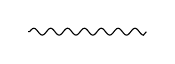
\begin{tikzpicture}
        \begin{feynman}
          \vertex (l);
          \vertex [right=of l] (r);
          \diagram*{
            (l) -- [photon] (r),
          };
        \end{feynman}
      \end{tikzpicture}
    \end{center}
    Each line comes with an index $i$ that tells us which component of $\mathbf{A}$ we are talking about. Each internal line gives us a factor of
    \[
      D_{ij}^{tr} = \frac{i}{p^2 + i \varepsilon} \left(\delta_{ij} - \frac{p_i p_j}{|\mathbf{p}|^2}\right),
    \]
    while for each external line,
     \begin{center}
      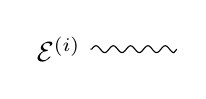
\begin{tikzpicture}
        \begin{feynman}
          \vertex (l) {$\mathcal{E}^{(i)}$};
          \vertex [right=of l] (r);
          \diagram*{
            (l) -- [photon] (r),
          };
        \end{feynman}
      \end{tikzpicture}
    \end{center}
    we simply write down a polarization vector $\mathcal{E}^{(i)}$ corresponding to the polarization of the particle.

  \item The $e \mathbf{j}\cdot \mathbf{A}$ term gives us an interaction of the form
    \begin{center}
      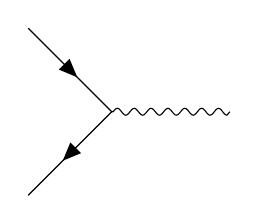
\begin{tikzpicture}
        \begin{feynman}
          \vertex (m);
          \vertex [above left=of m] (i1);
          \vertex [below left=of m] (i2);
          \vertex [right=of m] (f);

          \diagram*{
            (i1) -- [fermion] (m) -- [fermion] (i2),
            (m) -- [photon] (f),
          };
        \end{feynman}
      \end{tikzpicture}
    \end{center}
    This contributes a factor of $-ie\gamma^i$, where $i$ is the index of the squiggly line.

  \item The non-local term of the Lagrangian gives us instantaneous non-local interactions, denoted by dashed lines:
    \begin{center}
      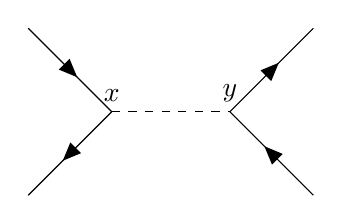
\begin{tikzpicture}
        \begin{feynman}
          \vertex (m1);
          \vertex [above left=of m1] (i1);
          \vertex [below left=of m1] (i2);
          \vertex [right=of m1] (m2);
          \vertex [above right=of m2] (f1);
          \vertex [below right=of m2] (f2);

          \diagram*{
            (i1) -- [fermion] (m1) -- [fermion] (i2),
            (f2) -- [fermion] (m2) -- [fermion] (f1),
            (m1) -- [scalar] (m2),
          };
          \node at (m1) [above] {$x$};
          \node at (m2) [above] {$y$};
        \end{feynman}
      \end{tikzpicture}
    \end{center}
    The contribution of this factor, in position space, is given by
    \[
      \frac{i(e \gamma_0)^2 \delta(x^0 - y^0)}{4\pi|\mathbf{x} - \mathbf{y}|}.
    \]
\end{enumerate}
Whoa. What is this last term saying? Recall that when we previously derived our Feynman rules, we first obtained some terms from Wick's theorem that contained things like $e^{ip\cdot x}$, and then integrated over $x$ to get rid of these terms, so that the resulting formula only included momentum things. What we've shown here in the last rule is what we have before integrating over $x$ and $y$. We now want to try to rewrite things so that we can get something nicer.

We note that this piece comes from the $A_0$ term. So one possible strategy is to make it into a $D_{00}$ piece of the photon propagator. So we treat this as a photon indexed by $\mu = 0$. We then rewrite the above rules and replace all indices $i$ with $\mu$ and let it range over $0, 1, 2, 3$.

To do so, we note that
\[
  \frac{\delta(x^0 - y^0)}{4\pi |\mathbf{x} - \mathbf{y}|} = \int \frac{\d^4 p}{(2\pi)^4} \frac{e^{ip\cdot(x - y)}}{|\mathbf{p}|^2}.
\]
We now define the $\gamma$-propagator
\[
  D_{\mu\nu}(p) =
  \begin{cases}
    \frac{i}{p^2 + i\varepsilon} \left(\delta_{\mu\nu} - \frac{p_\mu p_\nu}{|\mathbf{p}|^2}\right) & \mu, \nu \not= 0\\
    \frac{i}{|\mathbf{p}|^2} & \mu = \nu = 0\\
    0 & \text{otherwise}
  \end{cases}
\]
We now have the following Feynman rules:
\begin{enumerate}
  \item The photons are denoted as squiggly lines:
    \begin{center}
      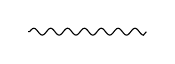
\begin{tikzpicture}
        \begin{feynman}
          \vertex (l);
          \vertex [right=of l] (r);
          \diagram*{
            (l) -- [photon] (r),
          };
        \end{feynman}
      \end{tikzpicture}
    \end{center}
    Each internal line comes with an index $\mu$ ranging over $0, 1, 2, 3$ that tells us which component of $\mathbf{A}$ we are talking about, and give us a factor of $D_{\mu\nu}$, while for each external line,
     \begin{center}
      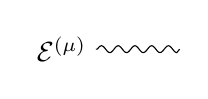
\begin{tikzpicture}
        \begin{feynman}
          \vertex (l) {$\mathcal{E}^{(\mu)}$};
          \vertex [right=of l] (r);
          \diagram*{
            (l) -- [photon] (r),
          };
        \end{feynman}
      \end{tikzpicture}
    \end{center}
    we simply write down a polarization vector $\mathcal{E}^{(\mu)}$ corresponding to the polarization of the particle.

  \item The $e \mathbf{j}\cdot \mathbf{A}$ term gives us an interaction of the form
    \begin{center}
      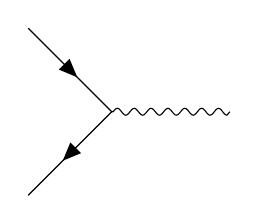
\begin{tikzpicture}
        \begin{feynman}
          \vertex (m);
          \vertex [above left=of m] (i1);
          \vertex [below left=of m] (i2);
          \vertex [right=of m] (f);

          \diagram*{
            (i1) -- [fermion] (m) -- [fermion] (i2),
            (m) -- [photon] (f),
          };
        \end{feynman}
      \end{tikzpicture}
    \end{center}
    This contributes a factor of $-ie\gamma^i$, where $i$ is the index of the squiggly line.
\end{enumerate}

Now the final thing to deal with is the annoying $D_{\mu\nu}$ formula. We claim that it can always be replaced by
\[
  D_{\mu\nu}(p) = -i \frac{\eta_{\mu\nu}}{p^2},
\]
i.e.\ in all contractions involving $D_{\mu\nu}$ we care about, contracting with $D_{\mu\nu}$ gives the same result as contracting with $-i \frac{\eta_{\mu\nu}}{p^2}$. This can be proved in full generality using momentum conservation, but we will only look at some particular cases.

\begin{eg}
  Consider the process
  \[
    e^- e^- \to e^- e^-.
  \]
  We look at one particular diagram
  \begin{center}
    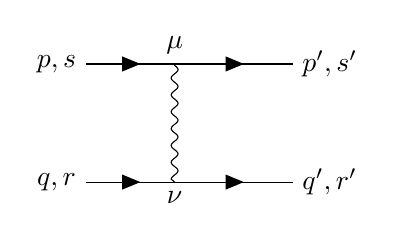
\begin{tikzpicture}
      \begin{feynman}
        \vertex (i1) {$p, s$};
        \vertex [below=of i1] (i2) {$q, r$};
        \vertex [right=of i1] (m1);
        \vertex [right=of i2] (m2);
        \vertex [right=of m1] (f1) {$p', s'$};
        \vertex [right=of m2] (f2) {$q', r'$};

        \node [above] at (m1) {$\mu$};
        \node [below] at (m2) {$\nu$};

        \diagram*{
          (i1) -- [fermion] (m1) -- [fermion] (f1),
          (i2) -- [fermion] (m2) -- [fermion] (f2),
          (m1) -- [photon] (m2),
        };
      \end{feynman}
    \end{tikzpicture}
  \end{center}
  We have two vertices, which contribute to a term of
  \[
    e^2 [\bar{u}(p') \gamma^\mu u(p)] D_{\mu\nu}(k)[\bar{u}(q') \gamma^\nu u(q)],
  \]
  where
  \[
    k = p - p' = -q + q'.
  \]
  We show that in this case, we can replace $D_{\mu\nu}(k)$ by
  \[
    D_{\mu\nu}(k) = \frac{-i \eta_{\mu\nu}}{k^2}.
  \]
  The proof follows from current conservation. Recall that $u(p)$ satisfies
  \[
    (\slashed p - m) u(p) = 0.
  \]
  We define the spinor combinations
  \begin{align*}
    \alpha^\mu &= \bar{u}(p') \gamma^\mu u(p)\\
    \beta^\mu &= \bar{u}(q') \gamma^\mu u(q)
  \end{align*}
  What we have is that
  \[
    k_\mu \alpha^\mu = \bar{u} (p')(\slashed p' - \slashed p) u(p) = \bar{u}(p')(m - m) u(p) = 0.
  \]
  Similarly, $k_\mu \beta^\mu$ is also zero. So our Feynman diagram is given by
  \[
    \alpha^\mu D_{\mu\nu} \beta^\nu = i\left(\frac{\boldsymbol\alpha \cdot \boldsymbol\beta}{k^2} - \frac{(\boldsymbol\alpha\cdot \mathbf{k})(\boldsymbol\beta \cdot \mathbf{k})}{|\mathbf{k}|^2 k^2} + \frac{\alpha^0 \beta^0}{|\mathbf{k}|^2}\right).
  \]
  But we know that $\alpha^\mu k_\mu = \beta^\mu k_\mu = 0$. So this is equal to
  \begin{align*}
    &\hphantom{=}i\left(\frac{\boldsymbol\alpha \cdot \boldsymbol\beta}{k^2} - \frac{k_0^2 \alpha^0 \beta^0}{|\mathbf{k}|^2 k^2} + \frac{\alpha^0 \beta^0}{|\mathbf{k}|^2}\right)\\
    &= i\left(\frac{\boldsymbol \alpha\cdot \boldsymbol\beta}{k^2} - \frac{1}{|\mathbf{k}|^2 k^2}(k_0^2 - k^2) \alpha^0 \beta^0\right)\\
    &= i\left(\frac{\boldsymbol \alpha\cdot \boldsymbol\beta}{k^2} - \frac{|\mathbf{k}|^2}{|\mathbf{k}|^2 k^2} \alpha^0 \beta^0\right)\\
    &= -i \frac{\alpha \cdot \beta}{k^2} \\
    &= \alpha^\mu \left(\frac{-i \eta_{\mu\nu}}{k^2}\right)\beta^\nu.
  \end{align*}
  What really is giving us this simple form is current conservation.
\end{eg}
In general, in Lorenz gauge, we have
\[
  D_{\mu\nu} = -\frac{i}{p^2} \left(\eta_{\mu\nu} + (\alpha - 1) \frac{p_\mu p_\nu}{p^2}\right),
\]
and the second term cancels in all physical processes, for similar reasons.

\subsubsection*{Charged scalars}
We quickly go through the Feynman rules for charged complex scalar fields. We will not use these for anything. The Lagrangian coming from minimal coupling is
\[
  \mathcal{L} = (\D_\mu \psi)^\dagger \D^\mu \psi - \frac{1}{4} F_{\mu\nu}F^{\mu\nu}
\]
We can expand the first term to get
\[
  (\D_\mu \psi)^\dagger \D^\mu \psi = \partial_\mu \psi^\dagger \partial^\mu \psi - ie A_\mu(\psi^\dagger \partial^\mu \psi - \psi \partial^\mu \psi^\dagger) + e^2 A_\mu A^\mu \psi^\dagger \psi.
\]
The Feynman rules for these are:
\begin{enumerate}
  \item The first interaction term gives us a possible vertex
    \begin{center}
      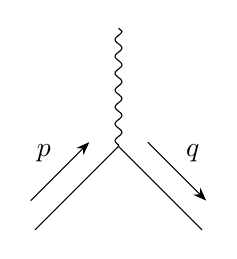
\begin{tikzpicture}
        \begin{feynman}
          \vertex (m);
          \vertex [below left=of m] (l);
          \vertex [below right=of m] (r);
          \vertex [above=of m] (t);
          \diagram*{
            (l) -- [momentum=$p$] (m) -- [momentum=$q$] (r),
            (m) -- [photon] (t),
          };
        \end{feynman}
      \end{tikzpicture}
    \end{center}
    This contributes a factor of $-ie(p + q)_\mu$.
  \item The $A_\mu A^\mu \psi^\dagger \psi$ term gives diagrams of the form
    \begin{center}
      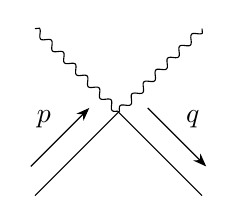
\begin{tikzpicture}
        \begin{feynman}
          \vertex (m);
          \vertex [below left=of m] (l);
          \vertex [below right=of m] (r);
          \vertex [above left=of m] (tl);
          \vertex [above right=of m] (tr);
          \diagram*{
            (l) -- [momentum=$p$] (m) -- [momentum=$q$] (r),
            (m) -- [photon] (tr),
            (m) -- [photon] (tl),
          };
        \end{feynman}
      \end{tikzpicture}
    \end{center}
    This contributes a factor of $2ie^2 \eta_{\mu\nu}$.
\end{enumerate}

\subsection{Computations and diagrams}
We now do some examples. Here we will not explain where the positive/negative signs come from, since it involves some tedious work involving going through Wick's theorem, if you are not smart enough to just ``see'' them.

\begin{eg}
  Consider the process
  \[
    e^- e^- \to e^- e^-.
  \]
  We again can consider the two diagrams
  \begin{center}
    \begin{tikzpicture}
      \begin{feynman}
        \vertex (i1) {$p, s$};
        \vertex [below=of i1] (i2) {$q, r$};
        \vertex [right=of i1] (m1);
        \vertex [right=of i2] (m2);
        \vertex [right=of m1] (f1) {$p', s'$};
        \vertex [right=of m2] (f2) {$q', r'$};

        \diagram*{
          (i1) -- [fermion] (m1) -- [fermion] (f1),
          (i2) -- [fermion] (m2) -- [fermion] (f2),
          (m1) -- [photon] (m2),
        };
        \node at (m1) [above] {$\mu$};
        \node at (m2) [below] {$\nu$};
      \end{feynman}
    \end{tikzpicture}
    \quad
    \begin{tikzpicture}
      \begin{feynman}
        \vertex (i1) {$p, s$};
        \vertex [below=of i1] (i2) {$q, r$};
        \vertex [right=of i1] (m1);
        \vertex [right=of i2] (m2);
        \vertex [right=of m1] (f1) {$p', s'$};
        \vertex [right=of m2] (f2) {$q', r'$};

        \diagram*{
          (i1) -- [fermion] (m1) -- [fermion] (f2),
          (i2) -- [fermion] (m2) -- [fermion] (f1),
          (m1) -- [photon] (m2),
        };
        \node at (m1) [above] {$\mu$};
        \node at (m2) [below] {$\nu$};
      \end{feynman}
    \end{tikzpicture}
  \end{center}
  We will do the first diagram slowly. The top vertex gives us a factor of
  \[
    -ie [\bar{u}^{s'}_{\mathbf{p}'}\gamma^\mu u^s_{\mathbf{p}}].
  \]
  The bottom vertex gives us
  \[
    -ie [\bar{u}^{r'}_{\mathbf{q}'} \gamma^\nu u^r_\mathbf{q}].
  \]
  The middle squiggly line gives us
  \[
    -\frac{i \eta_{\mu\nu}}{(p' - p)^2}.
  \]
  So putting all these together, the first diagram gives us a term of
  \[
    -i(-ie)^2 \left(\frac{[\bar{u}^{s'}_{\mathbf{p}'} \gamma^\mu u^s_\mathbf{p}][\bar{u}^{r'}_{\mathbf{q}'} \gamma_\mu u^r_\mathbf{q}]}{(p' - p)^2}\right).
  \]
  Similarly, the second diagram gives
  \[
    -i(-ie)^2 \left(\frac{[\bar{u}^{s'}_{\mathbf{p}'} \gamma^\mu u^s_\mathbf{q}][\bar{u}^{r'}_{\mathbf{q}'} \gamma_\mu u^r_\mathbf{p}]}{(p - q)^2}\right),
  \]
\end{eg}

\begin{eg}
  Consider the process
  \[
    e^+ e^- \to \gamma \gamma.
  \]
  We have diagrams of the form
  \begin{center}
    \begin{tikzpicture}
      \begin{feynman}
        \vertex (i1) {$p, s$};
        \vertex [below=of i1] (i2) {$q, r$};
        \vertex [right=of i1] (m1);
        \vertex [right=of i2] (m2);
        \vertex [right=of m1] (f1) {$\mathcal{E}^\mu, p'$};
        \vertex [right=of m2] (f2) {$\mathcal{E}^\nu, q'$};

        \diagram*{
          (i1) -- [fermion] (m1) -- [fermion] (m2) -- [fermion] (i2),
          (m1) -- [photon] (f1),
          (m2) -- [photon] (f2),
        };
      \end{feynman}
    \end{tikzpicture}
  \end{center}
  This diagram gives us
  \[
    i(-ie)^2 \left(\frac{[\bar{v}^r_{\mathbf{q}} \gamma^\nu(\slashed p - \slashed p' + m) \gamma^{\mu} u^s_{\mathbf{p}}]}{(p - p')^2 - m^2}\right) \mathcal{E}^\mu(\mathbf{p}') \mathcal{E}^\nu(\mathbf{q}').
  \]
  Usually, since the mass of an electron is so tiny relative to our energy scales, we simply ignore it.
\end{eg}

\begin{eg}[Bhabha scattering]
  This is definitely not named after an elephant.

  We want to consider the scattering process
  \[
    e^+ e^- \to e^+ e^-
  \]
  with diagrams
  \begin{center}
    \begin{tikzpicture}[yscale=0.5]
      \begin{feynman}
        \vertex (m1);
        \vertex [below=of m1] (m2);

        \vertex [left=of m1] (i1) {$p, s$};
        \vertex [left=of m2] (i2) {$q, r$};
        \vertex [right=of m1] (f1) {$p', s'$};
        \vertex [right=of m2] (f2) {$q', r'$};

        \diagram*{
          (i1) -- [fermion] (m1) -- [fermion] (f1),
          (i2) -- [anti fermion] (m2) -- [anti fermion] (f2),
          (m1) -- [photon] (m2),
        };
      \end{feynman}
    \end{tikzpicture}
    \quad
    \begin{tikzpicture}
      \begin{feynman}
        \vertex (m1);
        \vertex [above left=of m1] (i1) {$p, s$};
        \vertex [below left=of m1] (i2) {$q, r$};
        \vertex [right=of m1] (m2);
        \vertex [above right=of m2] (f1) {$p', s'$};
        \vertex [below right=of m2] (f2) {$q', r'$};

        \diagram*{
          (i1) -- [fermion] (m1) -- [fermion] (i2),
          (f2) -- [fermion] (m2) -- [fermion] (f1),
          (m1) -- [photon] (m2),
        };
      \end{feynman}
    \end{tikzpicture}
  \end{center}
  These contribute
  \[
    -i(-i e)^2 \left(-\frac{[\bar{u}^{s'}_{\mathbf{p}'} \gamma^\mu u^s_{\mathbf{p}}][\bar{v}^r_{\mathbf{q}} \gamma_\mu v^{r'}_{\mathbf{q}'}]}{(p - p')^2} + \frac{[\bar{v}^r_{\mathbf{q}} \gamma^\mu u^s_{\mathbf{p}}][\bar{u}^{s'}_{\mathbf{p}'} \gamma_\mu v^{r'}_{\mathbf{q}'}]}{(p + q)^2}\right).
  \]
\end{eg}

\begin{eg}[Compton scattering]
  Consider scattering of the form
  \[
    \gamma e^- \to \gamma e^-.
  \]
  We have diagrams
  \begin{center}
    \begin{tikzpicture}
      \begin{feynman}
        \vertex at (0, 0) (a);
        \vertex at (1.5, 0) (b);
        \vertex at (3, 0) (c);
        \vertex at (4.5, 0) (d);

        \node at (a) [left] {$u_{\mathbf{q}}$};
        \node at (d) [right] {$\bar{u}_{\mathbf{q}'}$};

        \vertex at (0, 1.5) (l) {$\mathcal{E}^\mu(\mathbf{p})$};
        \vertex at (4.5, 1.5) (r) {$\mathcal{E}^\nu(\mathbf{p'})$};

        \diagram*{
          (a) -- [fermion] (b) -- [fermion, momentum=$p + q$] (c) -- [fermion] (d),
          (l) -- [photon] (b),
          (c) -- [photon] (r),
        };
      \end{feynman}
    \end{tikzpicture}
    \quad\quad
    \begin{tikzpicture}
      \begin{feynman}
        \vertex at (0, 0) (a);
        \vertex at (1.5, 0) (b);
        \vertex at (3, 0) (c);
        \vertex at (4.5, 0) (d);

        \node at (a) [left] {$u_{\mathbf{q}}$};
        \node at (d) [right] {$\bar{u}_{\mathbf{q}'}$};

        \vertex at (1, 1.5) (l) {$\mathcal{E}^\mu(\mathbf{p})$};
        \vertex at (3.5, 1.5) (r) {$\mathcal{E}^\nu(\mathbf{p'})$};

        \diagram*{
          (a) -- [fermion] (b) -- [fermion, momentum'=$q - p'$] (c) -- [fermion] (d),
          (l) -- [photon] (c),
          (b) -- [photon] (r),
        };
      \end{feynman}
    \end{tikzpicture}
  \end{center}
\end{eg}

\begin{eg}
  Consider the
  \[
    \gamma\gamma \to \gamma\gamma
  \]
  scattering process. We have a loop diagram
  \begin{center}
    \begin{tikzpicture}
      \begin{feynman}
        \vertex (tl);
        \vertex [below=of tl] (bl);
        \vertex [right=of tl] (tr);
        \vertex [below=of tr] (br);
        \vertex [above left=of tl] (ttll);
        \vertex [above right=of tr] (ttrr);
        \vertex [below left=of bl] (bbll);
        \vertex [below right=of br] (bbrr);

        \diagram*{
          (tl) -- [fermion] (tr) -- [fermion] (br) -- [fermion] (bl) -- [fermion] (tl),
          (tl) -- [photon] (ttll),
          (bl) -- [photon] (bbll),
          (tr) -- [photon] (ttrr),
          (br) -- [photon] (bbrr),
        };
      \end{feynman}
    \end{tikzpicture}
  \end{center}
  Naively, we might expect the contribution to be proportional to
  \[
    \int \frac{\d^4 k}{k^4},
  \]
  This integral itself diverges, but it turns out that if we do this explicitly, the gauge symmetry causes things to cancel out and renders the diagram finite.
\end{eg}

\begin{eg}[Muon scattering]
  We could also put muons into the picture. These behave like electrons, but are actually different things. We can consider scattering of the form
  \[
    e^- \mu^- \to e^- \mu^-
  \]
  This has a diagram
  \begin{center}
    \begin{tikzpicture}[yscale=0.5]
      \begin{feynman}
        \vertex (m1);
        \vertex [below=of m1] (m2);

        \vertex [left=of m1] (i1) {$e^-$};
        \vertex [left=of m2] (i2) {$e^-$};
        \vertex [right=of m1] (f1) {$\mu^-$};
        \vertex [right=of m2] (f2) {$\mu^-$};

        \diagram*{
          (i1) -- [fermion] (m1) -- [fermion] (f1),
          (i2) -- [fermion] (m2) -- [fermion] (f2),
          (m1) -- [photon] (m2),
        };
      \end{feynman}
    \end{tikzpicture}
  \end{center}
  We don't get the diagram obtained by swapping two particles because electrons are not muons.

  We can also get interactions of the form
  \[
    e^+ e^- \to \mu^+ \mu^-
  \]
  by
  \begin{center}
    \begin{tikzpicture}
      \begin{feynman}
        \vertex (m1);
        \vertex [above left=of m1] (i1) {$e^-$};
        \vertex [below left=of m1] (i2) {$e^+$};
        \vertex [right=of m1] (m2);
        \vertex [above right=of m2] (f1) {$\mu^-$};
        \vertex [below right=of m2] (f2) {$\mu^+$};

        \diagram*{
          (i1) -- [fermion] (m1) -- [fermion] (i2),
          (f2) -- [fermion] (m2) -- [fermion] (f1),
          (m1) -- [photon] (m2),
        };
      \end{feynman}
    \end{tikzpicture}
  \end{center}
\end{eg}

%\subsection{The Coulomb potential}
%Consider an $e^- e^- \to e^- e^-$ scattering process. In the relativistic limit, we have
%\[
% u(\mathbf{p}) \to \sqrt{m}
% \begin{pmatrix}
% \xi\\ \xi
% \end{pmatrix}.
%\]
%So
%\begin{align*}
% \bar{u}^s(\mathbf{p}') \gamma^0 u^r(\mathbf{p}) &\to 2m \delta^{r s'}\\
% \bar{u}^s(\mathbf{p}') \gamma^i u^r(\mathbf{p}) &\to 0
%\end{align*}
%We now work in this non-relativistic limit, and try to get out the Coulomb potential.
%
%We average over initial and final spins, and we end up with an amplitude
%\[
% \mathcal{A} \sim \frac{i e^2 (2m)^2}{|\mathbf{p} - \mathbf{p}'|^2}.
%\]
%When we turn that into a potential as a function of their separation (and skipping over thousands of steps), we get
%\[
% U(r) = e^2 \int \frac{\d^3 \mathbf{p}}{(2\pi)^3} \frac{e^{i\mathbf{p}\cdot \mathbf{r}}}{|\mathbf{p}|^2} = \frac{e^2}{4\pi r}.
%\]
%So we recover the Coulomb potential.
%
%What happens when we look at $e^+ e^- \to e^+ e^-$? Going through the same computations, we find that we get an extra minus sign, so we get negative the potential, and thus they repel.

\printindex
\end{document}
